\documentclass{USC-Thesis}
\usepackage{graphicx}
\usepackage{amsmath}
\usepackage{amsfonts}
\usepackage{amssymb}
\usepackage{algorithm}
%\usepackage{algorithmic}
%\usepackage{algorithmicx}
\usepackage{algpseudocode}


\let\oldlistofalgorithms = \listofalgorithms
\renewcommand{\listofalgorithms}{  
\newpage
    \addcontentsline{toc}{chapter}{\listalgorithmname}
    \pagestyle{plain}
    \begin{singlespace} 
    \oldlistofalgorithms
    \end{singlespace}}

\begin{document}

\title{Exploring and Mapping Confined and Sensor-Challenged Environments with Proprioception of a Robotic Snake 
       }

\author{Jacob Everist}
\major{Computer Science}
\month{January}
\year{2013}
\maketitle

\dedication
    \begin{quote}
        \raggedleft {\em to family}
    \end{quote}

\tableofcontents 	% Table Of Contents

\listoffigures	% List of figures

\listoftables	% List of tables

\listofalgorithms

\topmatter{Preface}  % Preface with acknowlegements, etc.
%\input{preface.tex}

\topmatter{Abstract}
In many real-world environments such as flooded pipes or caves, exteroceptive sensors, such as vision, range or touch, often fail to give any useful information for robotic tasks.  This may result from complete sensor failure or incompatibility with the ambient environment.  We investigate how proprioceptive sensors can help robots to successfully explore, map and navigate in these types of challenging environments.

Our approach is to use a snake robot with proprioceptive joint sensors capable of knowing its complete internal posture.  From this posture over time, we are able to sweep out the free space of confined pipe-like environments.  With the free space information, we incrementally build a map.  The success of mapping is determined by the ability to re-use the map for navigation to user-directed destinations.

We address the following challenges: 1) How does the robot move and locomote in a confined environment without exteroception?  2) How is the distance traveled by a snake robot measured with no odometry and no exteroception?  3) How does the robot sense the environment with only proprioception?  4)  How is the map built with the information available?  5) How is the map corrected for visiting the same location twice, i.e. loop-closing?  6)  How does the robot navigate and explore with the constructed map?

In order to move through the environment, the robot needs to have a solution for motion planning and collision-reaction.  In an exteroceptive approach, we would detect and avoid obstacles at a distance.  If collisions were made, touch sensors could detect them and we could react appropriately.  With only proprioceptive sensors, indirect methods are needed for reacting to obstacles.  A series of motion methods are used to solve these problems including compliant locomotion, compliant path-following, safe-anchoring, stability assurance, slip detection, and dead-end detection.  We show results demonstrating their effectiveness.

While moving through the environment, the snake robot needs some means of measuring the distance traveled.  Wheeled robots usually have some form of shaft encoder to measure rotations of the wheels to estimate distance traveled.  In addition, range or vision sensors are capable of tracking changes in the environment to estimate position of the robot.   GPS is not feasible because of its unreliable operation in underground environments.  Our proprioceptive approach achieves motion estimation by anchoring multiple points of the body with the environment and kinematically tracking the change in distance as the snake contracts and extends.   This gives us a rudimentary motion estimation method whose effectiveness we measure in a series of experiments.

Some method is needed to sense the environment.  In an exteroceptive approach, vision and range sensors would give us a wealth of information about the obstacles in the environment at great distances.  Touch sensors would give us a binary status of contact with an obstacle or not.  With only proprioceptive joint sensors, our approach is to kinematically compute the occupancy of the robot’s body in the environment and record the presence of free space over time.  Using this information, we can indirectly infer obstacles on the boundary of free space.  We show our approach and the sensing results for a variety of environmental configurations.

Combining the multiple snapshots of the local sensed free space, the robot needs a means of building a map.  In the exteroceptive approach, one would use the ability to sense landmark features at a distance and identify and merge their position across several views.  However, in a proprioceptive approach, all sensed information is local.  The opportunities for spotting landmark features between consecutive views are limited.  Our approach is to use the pose graph representation for map-building and add geometric constraints between poses that partially overlap.  The constraints are made from a combination of positional estimates and the alignment of overlapping poses.  We show the quality of maps in a variety of environments.

In the event of visiting the same place twice, we wish to detect the sameness of the location and correct the map to make it consistent.  This is often called the loop-closing or data association problem.  In the case of exteroceptive mapping, this is often achieved by finding a correspondence between sets of landmark features that are similar and then merging the two places in the map.  In the proprioceptive case, the availability of landmark features is scarce.   We instead develop an approach that exploits the properties of confined environments and detects loop-closing events by comparing local environmental topologies.  We show the results of loop-closing events in a variety of environmental junctions.

Once we have constructed the map, the next step is to use the map for exploration and navigation purposes.  In the exteroceptive case, navigating with the map is a localization problem, comparing the sensed environment with the mapped one.  This is also the approach in the proprioceptive case.  However, the localization accuracy along the length of a followed path is more uncertain, so our path-following algorithms are necessarily more robust to this eventuality.   In the exteroceptive case, the act of exploration can be achieved by navigating to the boundaries of the map with no obstacles.  In the proprioceptive case, exploration is achieved by following every tunnel or path until a dead-end is detected.  We show some environments that we successfully map and navigate, as well as some environments that require future work. 





% TODO
% 1) notation guide, definition of terms (pose, posture, reference)
% 2) wrap-up, related work, how is best for chapter 2
% 3) figures for chapter 2
% 4) introduction of contributions in chapter 1
% 5) make a better organization and better story of chapter 2


% CONVENTIONS:
% P_k is a pose, p_k is a point
% joint posture is a vector of joint angle \hat{\phi}
% segment posture is a vector of poses, each element the pose of the i'th segment in the snake
% C is a curve


% DEFINITIONS:
% Pipe is a tight space with a tunnel or corridor like topology.  Minimal open space, follows a path.
% Path is a curve that represents the medial axis of a single traversal of a pipe
% Junction is a confluence of 3 or more pipes
% Branching is the event of the curve of the medial axis of a pose differing from another curve by a sharp turn that takes it from tangent to close to orthogonal
% Curve is either a function or a set of points that describes a curve.  All curves are finite with a start and finish terminals




\mainmatter 		% Begin Body

\chapter{Introduction}
\section{Problem}

Environments such as pipes and caves are difficult to robotically map because they are opaque and confined.  An environment is opaque when external range and vision sensors are inoperable because of lighting conditions, environmental fluids, or tight proximity to obstacles.  An environment is confined when a robot’s mobility is restricted by the close proximity to multiple obstacles.

A solution to this problem would allow mapping and exploration of previously inaccessible environments.  An approach that is invariant to ambient fluid (air, water, muddy water) would significantly impact cave exploration and underground science by the access to still deeper and smaller cave arteries regardless of whether they are submerged in water.  Search and rescue operations would have additional tools for locating survivors in complicated debris piles or collapsed mines.  Utility service workers would be able to map and inspect pipe networks without having to excavate or interrupt services.

These environments often render range sensors ineffective due to occlusions, distortions, reflections, and time-of-flight issues.  Changing visibility and lighting conditions will impact the usefulness of vision sensors.  Hazardous environments may also damage fragile external touch sensors.  This forces us to rely on a strictly proprioceptive approach for building environmental information.  Such sensors include accelerometers and joint sensors.  This sensor information is by definition, highly local to the robot’s position and sets us at a disadvantage to other mapping approaches that traditionally build maps with large sweeps of range data.  We have fundamentally less information with which to build maps and make exploration decisions.

An unstructured and irregular environment will require an agile robot with an equally agile locomotion approach.  For instance, a wheeled robot may not be capable of traversing through a complicated cave artery or debris pile but a snake robot will be able to.  Also, the geometry of the robot should not limit its ability to navigate.  For instance, a spherical robot may be able to go through a pipe of sufficient diameter, but if there is a brief pinch in the passage, the robot will not be able to continue.  The robot should be able to reposition itself to fit within the contours of the environment.

Global positioning information is also unavailable because of the enclosed nature of the environment.  Therefore, any mapping method will need an accurate motion estimation approach for the robot.  Wheeled dead-reckoning may be very difficult or impossible if the environment is highly unstructured or otherwise untenable to a wheeled locomotion approach.  Another method must be found.

\section{Related Work}

The mapping of confined spaces is a recurring theme in the research literature.  Work has been done to navigate and map underground abandoned mines [Thrun04] with large wheeled robots traveling through the constructed corridors.  Although the environment is large enough to make use of vision and range sensors, its location underground makes the use of GPS technologies problematic.  

Robotic pipe inspection has been studied for a long time [Fukuda89], but usually requires that the pipe be evacuated. The robotic solutions are often tailored for a specific pipe size and pipe structure with accompanying sensors that are selected for the task.  Often the solutions are manually remote-controlled with a light and camera for navigation.

Other work has focused on the exploration of flooded subterranean environments such as sinkholes [Gary08] and beneath sea-ice or glaciers.  This involves the use of a submersible robot and underwater sonar for sensing.

Other work has approach the problem of identifying features in the absence of external sensors.  This work comes from the robotic grasping literature and is described as “contact detection”.  That is, the identification and reconstruction of object contacts from the joint sensors of the grasping end effector.  These include Kaneko, Grupen, Haidacher, Mimura.

Finally, in addition to our early 2009 paper on this concept [Everist09], another researcher tackled the problem of mapping a confined and opaque environment of a pipe junction in an oil well bore hole deep underground [Mazzini11].  Mazzini’s approach focuses on mapping one local area of the underground oil well and uses physical probing to reconstruct the local features while anchored to a single reference frame.  
 
\section{Approach}

In this thesis, we use a snake robot in a physics simulation environment to develop a theoretical framework to map confined spaces with no external sensors.  With our simulation running the Bullet physics engine, we create a number of flat pipe-like environments in which our robot will explore and map.

We choose a snake robot form as our mapping robot due to its flexibility in moving through tight spaces and the large number of joint sensors from which we can extract environmental information. By pushing against the walls on either side of the pipe to form anchors and pulling the body forward, we achieve snake locomotion with a variation on the biological snake concertina gait.

Though we do not simulate any sensor-inhibiting fluid in the environment or sensor-failure scenarios, we prohibit ourselves from using any type of external sensor, be it touch sensors, vision sensors, or range sensors such laser range-finders and sonar.  Additionally, we do not allow ourselves to use any type of global positioning system since it is not practical to expect GPS to function underground.  The only sensors we permit ourselves to use are joint sensors.

To build the features of the environment, our robot sweeps its body through the environment and captures the free space through its body posture.   The free space becomes our dominant feature in map-making.   We use the pose graph representation for map-making, where at each pose, we build a local free space map.  We choose the geometric constraints between poses to ensure the correctness of the map.

We present several example environments, and we demonstrate the robot’s mapping and navigation results using our framework.   Our metric for success for determining the quality of a map is measured by selecting a random location on the map and judging how well the robot reliably navigates to that location in the world.

\subsection{Experimental System}

We explicitly chose to develop our approach in a simulation environment in order to rapidly develop a theoretical framework to the problem of mapping without external sensing.  In future work, we will apply these techniques to physical robots.

We choose to use the Bullet physics engine (version 2.77) because it is free, open source, mature, and actively developed.  Though it is primarily designed for games and animation, it is acceptable to our robotics application.  Our primary requisites are simulation stability and accurate modeling of friction and contact forces.   True friction and contact modeling are not available to us without specially designed simulation software at a monetary and performance speed cost.  Our choice of Bullet gives us believable results so long as we do not demand too much and try to simulate challenging situations (e.g. high speed, high mass, 1000s of contact points).

\begin{figure}
\begin{center}
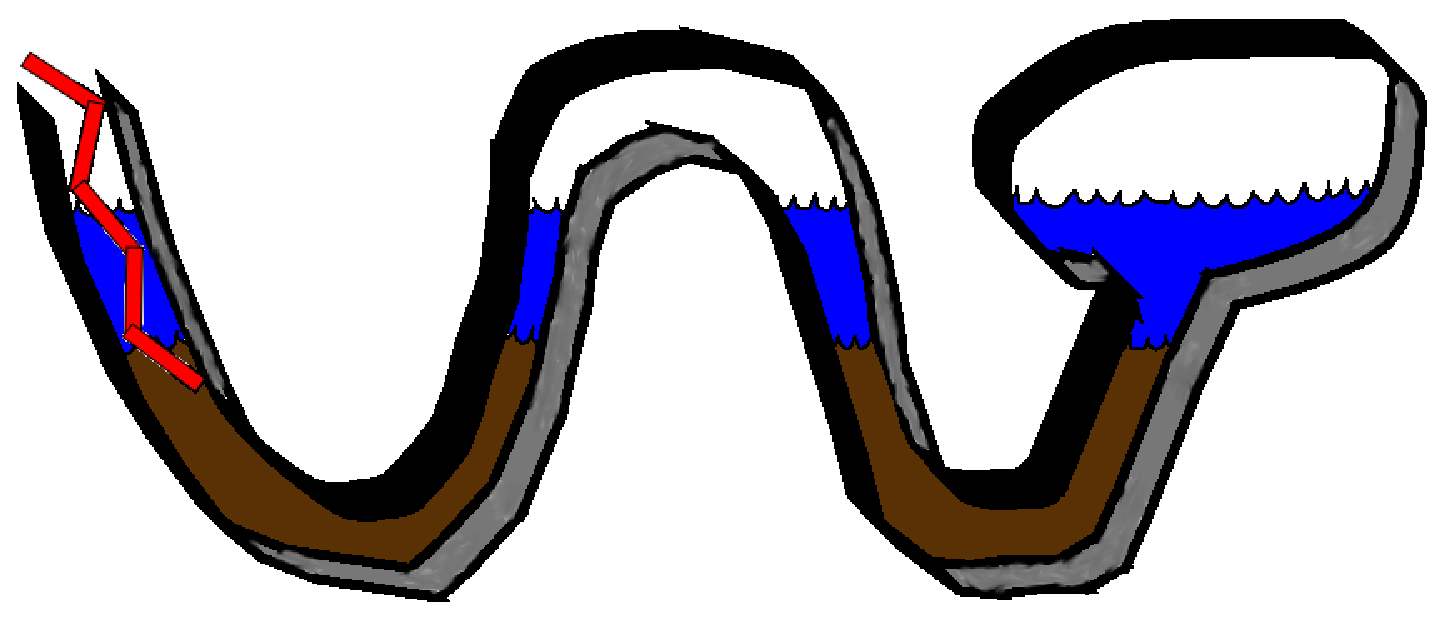
\includegraphics[scale=0.5]{rectv2-red.eps}
\end{center}
\caption{Example environment.}
\label{env1}
\end{figure}

We focus our attention on environments such as the one depicted in Figure \ref{env1}.  We build a flat plane and place a number of vertical walls to create a pipe-like maze environment.  All environments we study are flat and have no vertical components.  This means we need only focus on building 2D maps to represent the environment.  From here on in this paper, we refer to such environments as pipes even though they may not correspond to the even and regular structures of physical utility pipes.

A snake robot is placed in the pipe environment as shown in Figure \ref{env1}.  The snake robot consists of regular rectangular segments connected by actuated hinge joints.  Each of the joint axes is parallel and coming out of the ground plane.  This means the snake has no means to lift its body off the ground because all of its joints rotate in the plane of the ground.  It is only capable of pushing against the walls and sliding along the ground.  We choose a reduced capability snake robot because we wish to focus on the mapping problem instead of the more general serpentine control problem.

\begin{figure}
\begin{center}
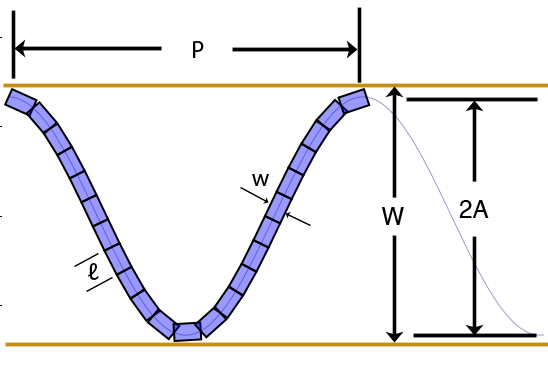
\includegraphics[scale=0.5]{CurveDiagram.png}
\end{center}
\caption{Definitions of snake and pipe parameters.}
\label{env2}
\end{figure}

We can parameterize the snake and the pipe environment.  For the snake robot, $l$ is the snake segment length, $w$ is the segment width, $N$ is the number of segments connected by $N-1$ joints, and $m$ is the maximum torque capable by each of the joint motors.

For the environment, we can begin by defining the pipe width $W$.  For a pipe with parallel and constant walls, this is a straightforward definition as seen in Figure \ref{env2}.  For non-regular features, we define the pipe width at a given point on one wall to be the distance to the closest point on the opposing wall.  This correctly captures the fact that a robot that is wider than the smallest pipe width $W$ will be unable to travel through that smallest width and will create a non-traversable pinch point.  Conversely, a pipe width $W$ that is larger than the reach of a robot will become a void space that the robot will have difficulty completely sensing without the aid of external sensors.  For both the minimum and maximum pipe widths of a given environment, we define $W_{min}$ and $W_{max}$ respectively where $W_{min} \leq W_i \leq W_{max}$ where $W_i$ is the pipe width at some point on wall $p_i$ of the pipe environment.

Each joint on the robot is actuated by a motor and PID controller.  It can actuate the joint anywhere from $\pm160$ degrees.   It uses the built-in motor capabilities of Bullet that allows us to set the joint angular velocity at run-time.  Therefore, all outputs of the PID controller set velocity commands to the joint and the physics engine does its best to satisfy those as velocity constraints.  


\begin{algorithm}
\caption{PID Controller}          % give the algorithm a caption
\label{alg1}
\begin{algorithmic}

\State $\epsilon \Leftarrow (\alpha - \phi)$

\If{$| \epsilon | > \mathrm{tol} $}

  \State $\epsilon_{sum} \Leftarrow \epsilon_{sum} + \delta t \times \epsilon$
  \State $\delta \epsilon \Leftarrow \epsilon-\epsilon_{last}$
  \State $\epsilon_{last} \Leftarrow \epsilon$
  \State $\hat{v} \Leftarrow \mathrm{P} \times \epsilon +\mathrm{I} \times \epsilon_{sum}+\mathrm{D} \times \delta \epsilon/\delta t$ 

  \If{$\hat{v} > v_{max}$}
    \State $\hat{v} \Leftarrow v_{max}$
  \EndIf
  \If{$\hat{v} < -v_{max}$}
    \State $\hat{v} \Leftarrow -v_{max}$
  \EndIf


\EndIf

\end{algorithmic}
\end{algorithm}

The structure of the PID controller is shown in Algorithm \ref{alg1}.  Line 1 defines the error as the difference between the target and the actual joint angle.  Line 2 prevents the controller from executing if the error falls below an acceptable threshold.  This prevents the motor from attempting to perform minor corrections to an already near-correct angle in order to avert oscillations or error-producing compensations.   Line 3 is the summation term for error over time while line 4 and 5 is the instantaneous error change from the previous controller iteration.  The actual PID control law is shown on line 6 where P is the proportional term coefficient, I is the integration term coefficient, and D is the derivative term coefficient.  The result outputs a command velocity for the Bullet engine.  Finally, lines 7-10 limit this velocity to a maximum.

Each of the joints gives angle position information to simulate a shaft encoder or potentiometer.  For this study, we do not simulate calibration error, sensor noise, resolution error, or gear backlash.  Calibration error has been studied elsewhere /cite and there exists correction mechanisms for it.  In the case of sensor noise, the noise on potentiometers is small enough not to affect our algorithms.  Gear backlash was encountered and studied in /cite Mazzini.  The primary error of concern is resolution error caused by the discretization process of a shaft encoder or an A/D converter.   This problem has been studied /cite.  Given a sensitive enough A/D converter (really?), this problem can be eliminated.  In this study, we assume correct and noise-free joint sensors.

A joint provides an API to the controlling program with 2 read-write parameters and 1 read-only parameter.  The read-write parameters are the target joint angle $\alpha_i$ and the maximum torque $m_i$, with the actual angle $\phi_i$ being the read-only parameter.  $\alpha_i$ is the angle in radians that we desire the joint to rotate to.  $\phi_i$ is the actual angle of the joint that reflects the current physical configuration of the robot.  $m_i$ is the maximum permitted torque that we wish to limit the individual motors to.  The maximum torque can be lowered to make the joints more compliant to the environment.



\section{Contributions}

Our contributions in this dissertation are the following:

\begin{itemize}
\item Snake movement without external sensors (Closed-loop control)
\item Proprioceptive odometer
\item Sensing with only proprioception
\item Build map with poses of local profiles that are not remotely sensible
\item Junction detection and loop-closing
\item Navigation and exploration with a proprioceptive map
\item Able to map and navigate several types of environments:  Y-junction, T-junction, X-junction, L-junction, etc.
\end{itemize}

We present our contributions in each of the subsequent chapters.




\chapter{Snake Locomotion without Exteroception}

\section{Problem}

FIXME: Related work and our contrasted difference.  What can we achieve that others cannot.  Why is our approach better for this particular case?  

In order to successfully control a snake robot and have it move through the environment, we need a solution for locomotion, motion planning, and handling collisions.  Since we have no exteroceptive sensors, this makes the problem challenging.  The robot is unable to sense what is right in front of it and must move blindly.  The snake could move into open space or collide with obstacles.

Part of the challenge is having no external sensors and the other part is general task-oriented control of a hyper-redundant robot.  There are many biologically-inspired locomotion strategies that live snakes in nature use to move throughout the environment.  The closest biological gait solution to moving in confined environments is the concertina gait shown in Figure \ref{bio}.

\begin{figure}
  \begin{center}
    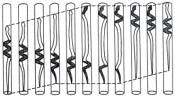
\includegraphics[width=3in]{concertina_gait_Gans1980.jpg}
  \end{center}
  \caption{Biological Concertina Gait of a Snake in a Confined Space.  Image taken from \cite{Gans:1980p775}}
	\label{bio}
\end{figure}

This gait is characterized by a concertina motion of alternating extensions and contractions that result in a forward movement. The snake body pushes against both sides of the walls establishing anchors that allow the snake to alternate between pulling and pushing itself forward. Success of locomotion depends on the snake establishing high friction contacts with the environment with which to push and pull.

However, the differences between a real snake and our robot snake make a true implementation impossible. A real snake has the luxury of vision and olfactory sensors to provide early motion planning and a rich tactile sensing surface skin to provide feedback to its control system. Our robot snake has only the benefit of internal proprioceptive joint sensors. If we knew the exact width of the pipe walls, we could prescribe the perfect concertina motion to move through the environment smoothly.

A simple approach to making the fully anchored concertina posture, we could use the following equation:

\begin{equation}
\label{eq:naiveconc}
\alpha_i = A * \cos \left( \frac{ 2 \pi if}{N} \right)
\end{equation}

where $\alpha_i$ is the commanded joint angle for joint $i$, $f$ is the frequency or the number of sinusoidal cycles per unit segment length, $A$ is the maximum joint command amplitude, and $N$ is the number of segments on the snake.   Since there are $N$ segments, there are $N-1$ joints.  Therefore, $i \in [0,N-1)$.  This equation requires some tuning to give the right results and can result in bad postures such as that shown in Figure \ref{naiveconc}.  In order to effect locomotion, a sliding Gaussian mask should be applied to the joint command output to transition parts of the snake between fully anchored to fully straight to reproduce the biological concertina gait.

\begin{figure}
\begin{center}
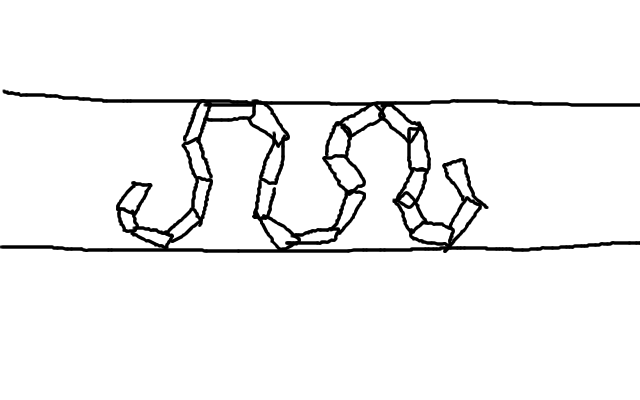
\includegraphics[scale=0.5]{2_problem_1.png}
\end{center}
\caption{Improperly tuned concertina posture using equation \ref{eq:naiveconc}.}
\label{naiveconc}
\end{figure}


The difficulty of this approach is that we need a priori knowledge of the pipe width, the configuration of the snake needs to be tuned by hand for the particular snake morphology, and there is no sensory feedback to this implementation.   With no feedback, there is no adaptive behavior possible.   We need an approach that will work in environments of unknown and variable pipe width.   Our robot needs to be able to adapt its locomotion to the width of the pipe.

Our desire is to be able to prescribe any type of snake posture, for any anchor width and any snake segment length or parameters, and have the snake automaticaly assume that posture.  In order to do this, we need a means of specifying the posture and an inverse kinematics method for achieving that posture.

For both of these requirements, we use the backbone curve-fitting methodology first described by \cite{Chirikijan:1995p774}.  This method of control is to produce a parameterized curve that represents the desired posture of the snake over time. Over time the curve changes to reflect desired changes in the snake posture. Snake backbone curve fitting is achieved by finding the joint positions that best fit the snake body onto the curve. This is found either by direct calculation or a search algorithm.

An example of backbone curve fitting can be seen in Figure \ref{onePeriod}.   The parameterized curve is shown in light blue in the background.   The blue snake body in the foreground is fitted onto the curve using an iterative search algorithm for each consecutive joint. 

\begin{figure}
  \begin{center}
    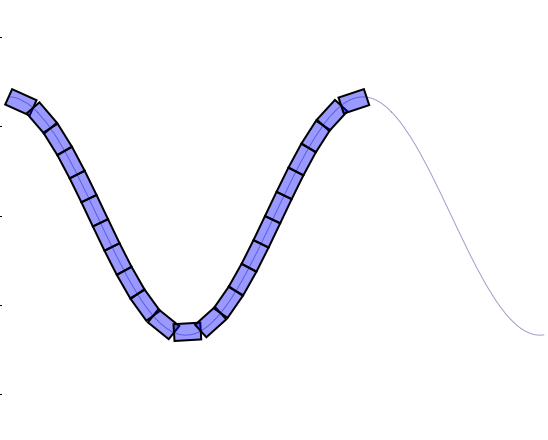
\includegraphics[width=3in]{OnePeriodCurve.png}
  \end{center}
  \caption{One sine period curve}
	\label{onePeriod}
\end{figure}

A typical application would be to specify the posture of the snake using a sinusoidal curve and then applying an inverse kinematics technique to fit the snake to the curve.   The problem can be formulated iteratively as follows: for joints $i \in [0,k]$ and joint pose in space $p_i = \langle x_i,y_i,\theta_i \rangle $ are on the curve $\beta$ with parameter $t_i$, find the joint angle $a_k$ such that $p_{k+1}$ is on the curve $\beta$ and $t_k < t_{k+1}$.

For the equation $\beta$ defined as:
\begin{equation}
\label{eq:curve1}
y = A\sin(2\pi x)
\end{equation}

the equation is monotonic along the $x$ axis, so satisfying the criteria $t_i < t_{i+1}$ is the same as satisfying $x_i < x_{i+1}$.  

If the length a of snake segment is $l$, we specify a circle equation centered at the joint position $(x_i,y_i)$ with the following:

\begin{equation}
\label{eq:IKcircle}
(x-x_i)^2 + (y-y_i)^2 = l
\end{equation}

Finding solutions for the simultaneous equations \ref{eq:curve1} and \ref{eq:IKcircle} will give us possible solutions to $x_{i+1}$ and $y_{i+1}$.  For these two sets of equations, there are always at least 2 possible solutions.  We need only select the solution that satisfies the invariant condition $x_i < x_{i+1}$.   There may be more than solution.  In which case, we select the $x_{i+1}$ where $(x_{i+1}-x_i)$ is the smallest.  This prevents the snake from taking shortcuts across the curve and forces it to fit as closely as feasibly possible to the parameterized curve given the snake robot’s dimensions.

The above simultaneous equations do not have closed-form solutions and instead must be solved numerically.  This can be computationally expensive using general equation solvers.  Instead we propose a more specialized solver for this particular problem.

We choose a series of uniform samples $(q_0 ... q_k ... q_M)$ around a circle of radius $l$ centered at $(x_i,y_i)$ such that all points $q_k$ have $x_k >= x_i$.  We are looking for instance of crossover events where the line segment $(q_k,q_{k+1})$ crosses over the curve $\beta$.   Given at least one crossover event, we do a finer search between $(q_k, q_{k+1})$ to find the closest point on the circle to the curve $\beta$ and accept that as our candidate position for joint point $p_{k+1}$.   As long as we assume that the curve $\beta$ is monotonic along the x-axis and a point of the curve $\beta$ can be computed quickly given an x-value, this is a faster method of computing intersections of the circle with the backbone curve than a general numerical solver.

For instance, in Figure \ref{plot_3}, we show a curve $\beta$ described by a sine curve and a series of circles intersecting with the curve that indicate candidate locations for placing the subsequent joint on the curve.  These are used to determine the appropriate joint angles to fit the snake onto the curve.

Now that we have a means of changing the snake’s posture to any desired form given a parameterized, monotonic curve that describes the posture, we now need to form an anchoring approach that will work for arbitrary pipe widths.


\section{Anchoring}

In order to fit the anchor points to a pipe of unknown width, we need some way of sensing the walls.  Since we have no exteroceptive sensors, the best way of sensing the width of the walls is by contact.  Since we have no direct contact sensor per se, we must detect contact indirectly through the robot’s proprioceptive joint sensors.

Using the backbone curve fitting approach, we take one period of a sine curve as the template form we wish the robot to follow.  We then modify this sine period’s amplitude, at each step refitting the snake robot to the larger amplitude, until the robot make’s contact with the walls.  This establishes two points of contact with the wall which assist in immobilizing the snake body.

It is clear from Figure \ref{onePeriod} that as the amplitude of the curve increases, more segments are needed to complete the curve.  If the sine curve is rooted at the tip of the snake, this results in the curve translating towards the snake’s center of mass.  Instead, we root the sine curve on an internal segment, as seen in Figure \ref{anchor1}, so that the position of the anchor points remain relatively fixed no matter the amplitude and the number of segments required to fit the curve.

\begin{figure}
\begin{center}
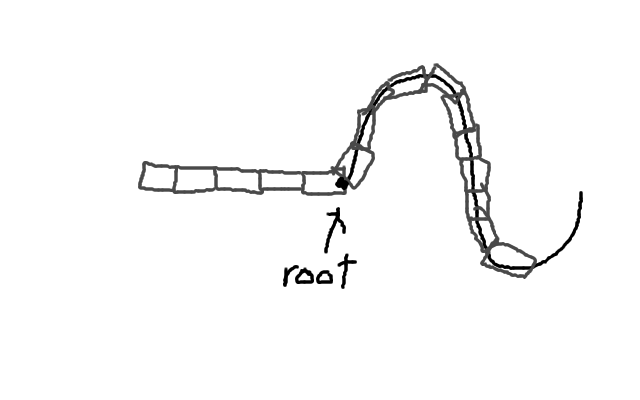
\includegraphics[scale=0.5]{2_anchoring_1.png}
\end{center}
\caption{Anchor with not enough segments}
\label{anchor1}
\end{figure}

\begin{figure}
\begin{center}
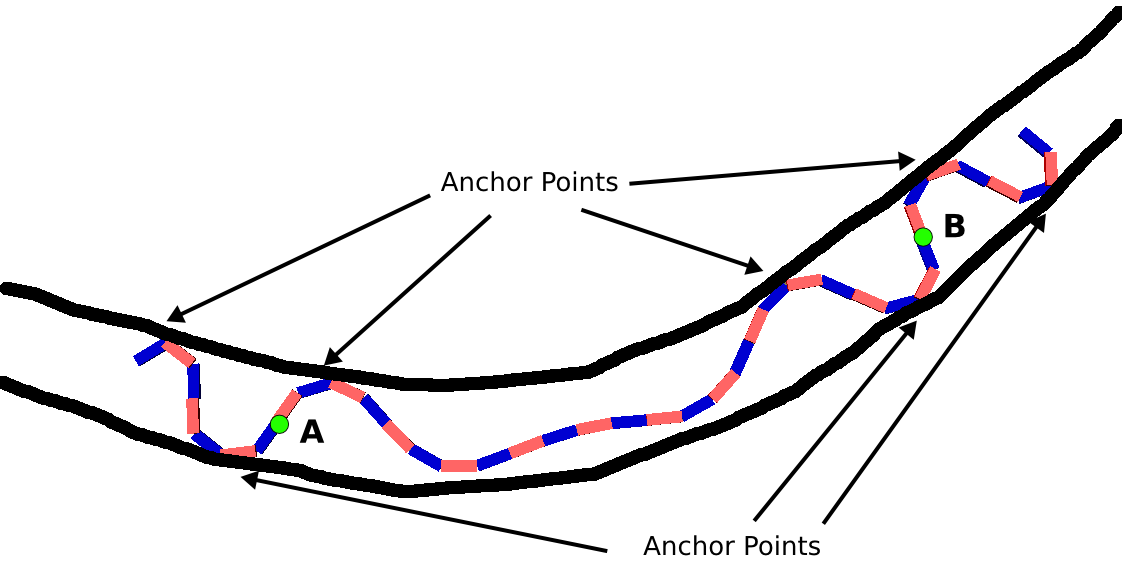
\includegraphics[scale=0.4]{ref_points_pose2.png}
\end{center}
\caption{Anchor Points}
\label{fig:anchor_points}
\end{figure}


Two points of contact are not statically stable if we disregard friction.  Though friction exists in our simulation and in reality, we do not rely on it to completely immobilize our robot.  Our normal forces are often small and the dynamic and transient forces can easily cause a contact slip.  Therefore, we need at least 3 contact points to consider an anchor to be statically stable.

One way to achieve this is by adding new sine period sections to create another pair of anchors.  The amplitude of the new sine period is separate from the previous anchor’s amplitude and is represented by a new curve attached to the previous one. This way the amplitudes remain independent.  The equation to describe two sets of sine period curves with independently controlled amplitudes are as follows:

\begin{equation}
y = \mathrm{U}(x)  \mathrm{U}(2\pi-x) A_1 \sin(fx) + \mathrm{U}(x-2\pi) \mathrm{U}(4\pi-x) A_2 \sin(fx)
\end{equation}

where $f$ is the frequency and $\mathrm{U}(x)$ is a unit step function.  Or to generalize for $N$ periods and $N$ pairs of anchor points:

\begin{equation}
y = \sum_{i=0}^{N-1} \mathrm{U}(x-i 2\pi) \mathrm{U}((i+1) 2\pi-x) A_i \sin(fx)
\end{equation}


for each anchor curve amplitude $A_i$.

So now that we have the means to control the amplitude of our anchor points, we need some means of detecting that a contact is made and another to make sure the anchor is secure. 

Our approach is to gradually increase the amplitude of an anchor curve until contact with both walls has been made.  We will continue to increase the amplitude until we see significant joint error occur when fitting to the curve.  If the amplitude because larger than the width of the pipe, the snake will attempt fitting to a curve that is impossible to fit to and will experience a discrepancy in its joint positions compared to where it desires them to be.

The structure of this error will normally take the form of one or two large discrepancies surrounded by numerous small errors.  This reflects that usually one or two joints will seriously buckle against the wall, while the rest of the surrounding joints can reach their commanded position without disturbance.  An example of an anchor curve with larger amplitude than the width of the pipe is shown in Figure \ref{anchor2}.

\begin{figure}
\begin{center}
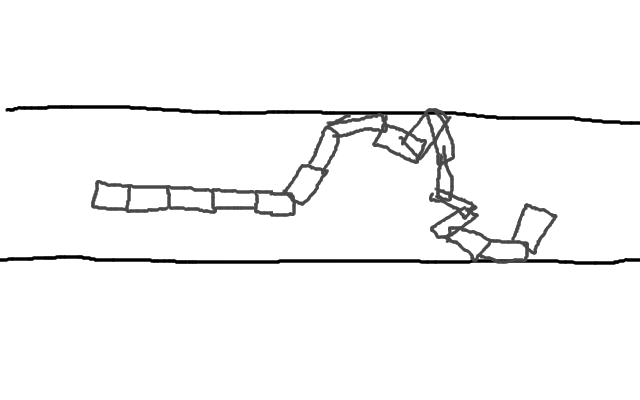
\includegraphics[scale=0.5]{2_anchoring_2.png}
\end{center}
\caption{Anchor with amplitude larger than pipe width.}
\label{anchor2}
\end{figure}

The contact is flagged once the maximum error reaches a certain threshold across all the joints of the anchor curve.  Of the joints $M$ of the anchor curve and the error $e_j$, if there exists $e_j > 0.3$ radians, than we flag a contact.  It isn’t so much that we are detecting a contact but a minimum pushing threshold against the wall.  The robot is pushing hard enough to cause joint error over an experimentally determined threshold.

If $j_k$ through $j_{k+M}$ are the joints comprising the fitted anchor curve, the error of one joint is defined by $e_k = |\phi_k-\alpha_k|$.  The maximum error is defined by $e_{max} = \mathrm{max}(e_k, e_{k+1} \cdots e_{k+M-1}, e_{k+M})$.

The amplitude is initially changed by large increments to quickly find the walls.  Once the threshold has been reached, the current and last amplitude are marked as the max and min amplitudes respectively.  We then proceed to perform a finer and finer search on the amplitudes between the max and min boundaries until we reach a snug fit that is just over the error threshold.  This is a kind of numerical search(?).

The pseudocode for this algorithm is as follows:


\begin{algorithm}
\caption{Anchor Fitting}          % give the algorithm a caption
\label{alg:anchor}
\begin{algorithmic}

\State $\hat{A} \Leftarrow 0$
\State $A_{min} \Leftarrow 0$
\State $A_{max} \Leftarrow \infty$
\State $\delta A \Leftarrow 0.04$

\While{$ (A_{max}-A_{min} >= 0.001) \And (\delta A >= 0.01)  $} 

  \State $\hat{A} \Leftarrow \hat{A} + \delta A$
  \State $e_{flag} \Leftarrow \mathrm{setAnchorAmp}(\hat{A})$
 
  \If { $\neg e_{flag}$ }
    \State $A_{min} \Leftarrow \hat{A}$
  \Else
    \State $A_{max} \Leftarrow \hat{A}$
    \State $\delta A \Leftarrow \delta A / 2$
    \State $\hat{A} \Leftarrow A_{min}$
    \State $\mathrm{setAnchorAmp}(\hat{A})$

  \EndIf

\EndWhile

\end{algorithmic}
\end{algorithm}

The main objective of this code is to reduce the difference between maxAmp and minAmp as much as possible.  minAmp and maxAmp are the closest amplitudes under and over the error threshold respectively.  The function setAnchorAmp() sets the amplitude, performs the curve fitting, and reports back any error condition as described earlier.  Once this algorithm is complete, we have made a successful anchor with two contact points under compression without the fitted anchor curve being distorted by joint buckling.

\section{Curves}

When we describe curves for use in backbone curve fitting, they must be assigned to a frame of reference and usually have a starting point.  Most often, the frame of reference chosen is one of the local segment frames on the snake body.  However, sometimes we could choose the global frame if we wanted to navigate or probe something specific in the environment.  The local frame curves that we use all start from a specific body segment and sprout from that segment like a plant.  We say that this curve is rooted in segment X. 


\section{Behaviors}

Our method of control is a behavior-based architecture that is charged with reading and tasking the servo-based motor controllers of each joint.  Each behavior may be a primitive low-level behavior or a high-level composite behavior composed of multiple sub-behaviors.  Furthermore, a behavior may have complete control of every joint on the snake or the joints may be divided between different but mutually supporting behaviors.  This architecture allows us to achieve a hierarchy of behavior design as well a separation of responsibilities in task achievement.  For instance, the back half of the robot could be responsible for anchoring, while the front half could be responsible for probing the environment as seen in the example architecture in Figure \ref{behaviors1}.

\begin{figure}
\begin{center}
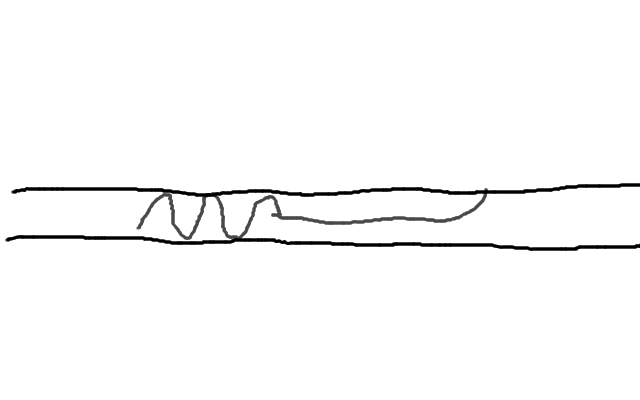
\includegraphics[scale=0.5]{2_behaviors_1.png}
\end{center}
\caption{Separation of functionality.}
\label{behaviors1}
\end{figure}

Each behavior in the behavior-based architecture is time-driven.  It is called periodically by a timer interrupt to compute the next commands for the following time-step.  This could be variable time or constant time, but to make our behavior design simple, we use 10ms constant time steps in our simulation.

At each time step, the state of the robot is captured and driven to the behaviors.  The data includes a vector of joint angles $\phi_i$, a vector of commanded angles $\alpha_i$, and a vector of maximum torques $m_i$.  These values were described in the previous section X.  The output of each behavior is a vector of new commanded angles $\hat{\alpha}_i$, a vector of new max torques $\hat{m}_i$, and a vector of control bits $c_i$.  The values of $\hat{\alpha}_i$ can be any radian value within the joint range of motion or it can be NULL.  Likewise, the new max torque of $\hat{m}_i$ can be any non-negative max torque threshold or NULL.  The NULL outputs indicate that this behavior is not changing the value and if it should reach the servo-controller, it should persist with the previous value.

The bits of the control vector, $c_i$ , are either 1, to indicate that the behavior is modifying joint i, or 0, to indicate that it has been untouched by the behavior since its initial position when the behavior was instantiated.  This control vector is to signal the activity to parent behavior that this part of the snake is being moved or controlled.  The parent behavior does not need to respect these signals, but they are needed for some cases.

Our behavior-based control architecture follows the rules of control subsumption.  That is, parent behaviors may override the outputs of child behaviors.  Since we can also run multiple behaviors in parallel on different parts of the snake, sometimes these behaviors will try to control the same joints.  When this happens, the parent behavior is responsible for either prioritizing the child behaviors or adding their own behavior merging approach.

Asymmetric behaviors that run on only one side of the snake such as the front are reversible by nature.  That is, their direction can be reversed and run on the back instead.  All behaviors with directional or asymmetric properties have this capability..

Finally, parent behaviors can instantiate and destroy child behaviors at will to fulfill their own control objective.  All behaviors are the child of some other behavior except the very top root-level behavior which is the main control program loaded into the robot and responsible for controlling every joint.  The root behavior is responsible for instantiating and destroying assemblages of behaviors to achieve tasks as specified in its programming.  We will discuss some of these behaviors and child behaviors in the following sections.

\section{Smooth Motion}
\label{sec:smooth}

We desire the motion of our snake robot to be slow and smooth in nature.  It does us no benefit for the motion to be sudden and jerky.  Moments of high acceleration can have unintended consequences that result in our anchor points slipping.  Either collisions with the environment or transient internal dynamics can cause the anchor points to slip.

Our method of ensuring smooth motion is to take the initial and target posture of the joints of the snake, perform linear interpolation between the two poses, and incrementally change the joint angles along this linear path.  For instance, if the initial joint angles are ${s_0 ... s_n}$ and the target joint angles are ${t_0 ... t_n}$, the interpolated path for each joint $j$ is found by $g_{jr} = s_j + (t_j – s_j) * (r/100)$ for $r \to {0, 100}$, for 100 interpolated points on the linear path.  The resultant motion is a smooth transition from initial to target posture as seen in Figure \ref{smooth1}.

\begin{figure}
\begin{center}
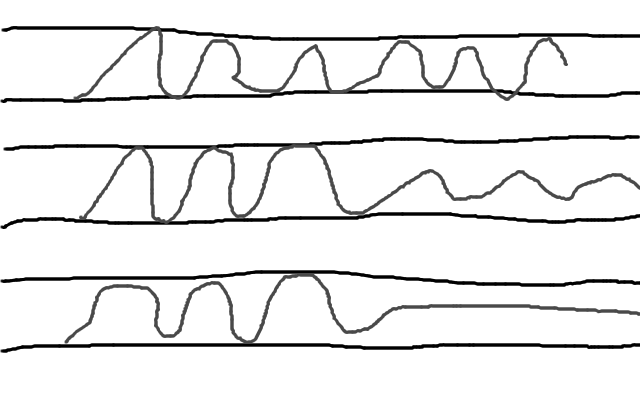
\includegraphics[scale=0.5]{2_smooth_1.png}
\end{center}
\caption{Smooth motion from interpolation of posture.}
\label{smooth1}
\end{figure}

This is the definition of the HoldTransition behavior.  When it is instantiated, it is given an initial pose vector $S$ and target pose $T$, where some values of $t_i$ in $T$ and $s_i$ in $S$ may have NULL for no command.   At each step of the behavior, using the equation $g_{jr} = s_j + (t_j – s_j) * (r/100)$, $r$ is incremented to compute the new joint command.  If $t_j$ is NULL, then $g_{jr} = s_j$.  Once $r = 100$, it returns True on step() and on all subsequent steps, $g_j = t_j$.


\section{Behavior Merging}

\label{sec:merge}

There are a few methods for merging behaviors that overlap in some way.  One way of the previous section is for two behaviors to overlap temporally and using the HoldTransition behavior to handle a smooth transition from one configuration to another.

In the event that two behaviors control adjacent sets of joints or overlap their control in some way, a conflict resolution is method is needed to not only select the proper command for contested joints, but to prevent either behavior from negatively affecting functionality of the other by modifying any positional assumptions or introducing any unintended forces or torques to the other side.

A common occurrence is that two behaviors may try to control the same set of joints at the same time or otherwise.  This is a conflict that requires resolution by the parent behavior.  In this section we present three different ways to merge the outputs of different behaviors as means of conflict resolution.  They are, in the order presented, the precedence merge, the splice merge, the convergence merge, and the compliance merge respectively.

Given that all child behaviors have an ordering, the default resolution method is to take the first behavior’s control output over all others.  This is called precedence merging.  An ordering is always specified by the parent at the time it instantiates the child behaviors.  If the first behavior’s output is NULL, then it goes to the next behavior and so on until a non-NULL value is found or the last behavior returns a NULL, in which case the parent also returns a NULL unless the parent otherwise specifies.

Precedence merging can be crude when trying to maintain a stable and immobilized position in the environment.  Sudden changes at the behavior-boundary can cause jarring discontinuities on the snake’s posture and result in loss of anchoring as seen in Figure \ref{merging1}.  A more finessed approach would disallow these discontinuities and provide a non-disruptive merging.  The first approach that does this is the splice merge.

\begin{figure}
\begin{center}
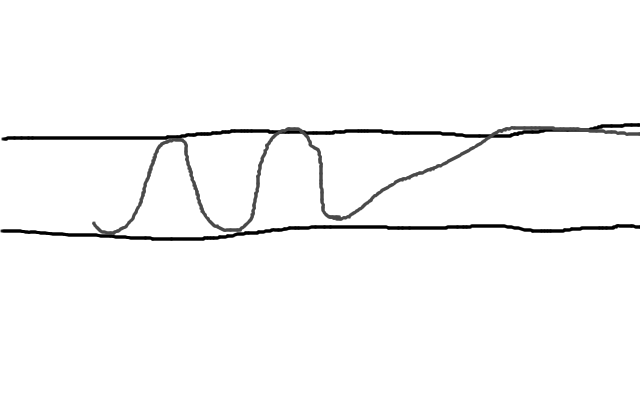
\includegraphics[scale=0.5]{2_merging_1.png}
\end{center}
\caption{Discontinuity in behaviors results in clash of functionality.}
\label{merging1}
\end{figure}

In the event that two behaviors overlap, we have the option of having a hard boundary between the behaviors centered on a single joint. Except in the rare case that both behaviors want to command the splice joint to the same angle, it is highly likely that the merge will be discontinuous.  In order to ensure that positional assumption is maintained for both behaviors, the behaviors must be spliced so that neither behavior disrupts the other.

If the splice joint is $j_s$, behavior A controls joints $j_0$ through $j_s$, behavior B controls joints $j_s$ through $j_{N-1}$, $S_{s-1}$ is the body segment connected to $j_s$ in behavior A, and $S_s$ is the body segment connected to $j_s$ in behavior B, we have the situation shown in Figure \ref{merging2}a.  If behavior A commands $j_s$ to $\alpha_a$ to put segment $S_s$ in the position shown in Figure \ref{merging2}b and conversely, if behavior B commands $j_s$ to $\alpha_b$ to put segment $S_{s-1}$ in the position shown in Figure \ref{merging2}c, the two behaviors can be spliced discontinuously with no disruption to either behavior by setting $j_s$ to $\alpha_s = \alpha_a + \alpha_b$.  The result is shown in Figure \ref{merging2}d.

\begin{figure}
\begin{center}
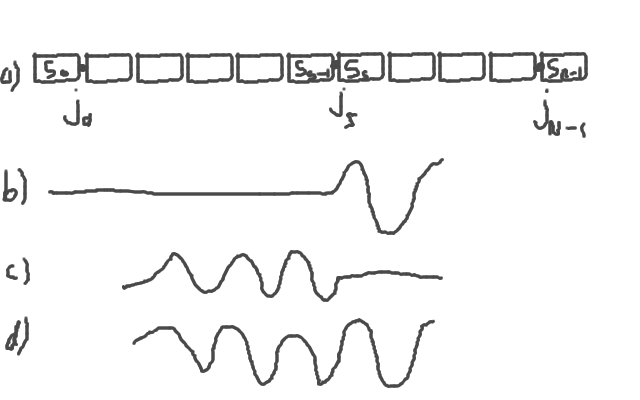
\includegraphics[scale=0.5]{2_behaviors_2.png}
\end{center}
\caption{Splice joint and connecting segments.}
\label{merging2}
\end{figure}

This is the behavior splicing approach because it stitches the behaviors together in a clinical way to ensure proper functionality of both.  Its primary role is to connect behaviors with discontinuous conflicts on the behavior boundary and whose positions must be maintained for functional purposes.  For more fuzzy continuous boundaries, we use the convergence merging approach.

For the two behaviors shown in Figure \ref{merging3}a and \ref{merging3}b, the resultant convergence merge is shown in Figure \ref{merging3}c.  For this approach, there is no discrete boundary but one behavior converging to another over several joints.  For a given joint $j_i$ somewhere in this convergence zone, and the commanded values for behaviors A and B being $\alpha_a$ and $\alpha_b$, the converged command value for $j_i$ is computed by:

\begin{equation}
\label{equ:slide}
\alpha_i = \alpha_a + (\alpha_b – \alpha_a) / ( 1 + \exp(i-c))
\end{equation}

where $c$ is a calibration parameter that controls the magnitude and location of the convergence along the snake.  As $c \to +\infty$, $\alpha_i \to \alpha_b$.  As $c \to -\infty$, $\alpha_i \to \alpha_a$.  In practice, $|c| < 20$ is more than sufficient for complete convergence to one behavior or the other.  The $i$ parameter in the exponent ensures that the convergence value is different for each of the neighboring joints.  This produces the effect shown in Figure \ref{merging3}c.

\begin{figure}
\begin{center}
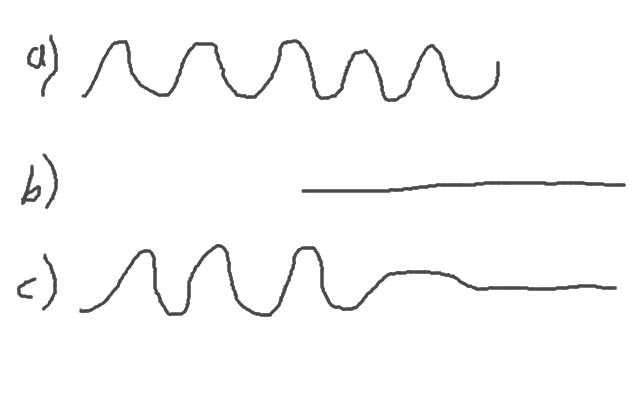
\includegraphics[scale=0.5]{2_behaviors_3.png}
\end{center}
\caption{Convergence merge.}
\label{merging3}
\end{figure}

If we modify $c$, this gives us a control knob on the merge and can be moved up and down.  If we move $c \to +\infty$, behavior B takes complete control of the snake.  If we move $c \to -\infty$, behavior A takes control of the snake.  $c$ can be changed over time to create a sliding transition effect with a convergence boundary.  In fact, this is the basis for a behavior called HoldSlideTransition.

A fourth and final way for two behaviors to be merged is the compliance merge.  This is the case where two behaviors are not adjacent but are far away from each other, but still interfere with each other somehow by inflicting unwanted forces and torques between the behaviors.

A compliance merge resolves this by selecting a group of joints between the two behavior’s joint sets to be compliant or non-actuated.  This has the result of absorbing any forces or torques transmitted by either behaviors and mechanically isolating one side of the snake from the other.  An example is shown in Figure \ref{merging4}.

\begin{figure}
\begin{center}
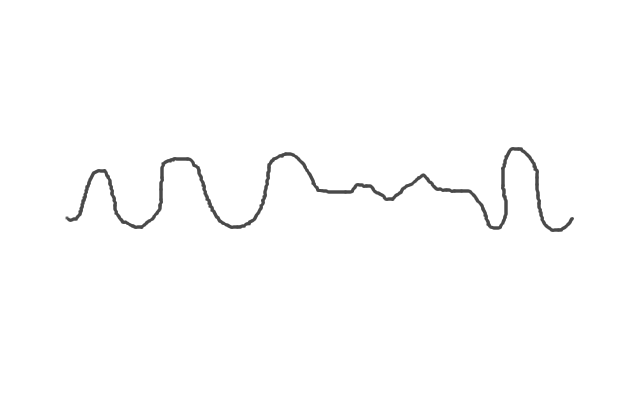
\includegraphics[scale=0.5]{2_behaviors_4.png}
\end{center}
\caption{Compliance merge.}
\label{merging4}
\end{figure}

\section{Compliant Motion}

In the previous section, we mentioned compliance but not our implementation.  Compliant motion is a much used technique in robotics and has been discussed widely (cite).  The two approaches are either passive or active compliance.  Our approach is to use passive compliance since we have no means to detect contact or sense obstacles.

Passive compliance is achieved by changing the settings on the max torque parameter of each joint’s servo controller.  We use a high setting for active motion, a low setting for compliant motion, and zero for keeping the joint unactuated.

Besides using a compliance merge to mechanically isolate two behaviors, we also use compliance as an exploration strategy.  Since we have no exteroception, the only way to discover walls and obstacles is to collide with them.  Compliant impacts with obstacles have a couple benefits.  It prevents the force of the impact from transmitting to the body of the snake and possibly causing anchor slip.   It also allows the joints of the snake to give out and take the shape of the environment around it.  

This latter benefit is one of our primary means of sensing and exploring the environment.  By passively letting the snake robot assume the shape of the environment, it guides our mapping and our locomotion.  Until we have mapped out open space and boundaries, we have no way of directing our robot towards them beyond colliding with the unknown.

\section{Stability Assurance}

\label{sec:stability}

In a previous section on smooth motion, we discussed an interpolation technique to smoothly transition from one posture to another.  The primary motive of this was to keep the parts of the snake body that are immobilized from being destabilized by transient forces and causing anchor slip.  Static forces from prolonged pushing against an obstacle or wall are a separate matter.

For a pose transition that has a sufficiently large number of interpolation steps of sufficiently large duration, we can reasonably be assured that no transient forces from dynamics or collision will cause anchor slip because we are moving very very slowly.  However, sufficiently long transition times for reliability may be impractical for applications, since times for a simple transition can be upwards of 1-2 minutes using a conservative approach.  For a robot that performs hundreds of moves that require transitions, this is an unacceptable approach.

If we focus on being able to detect transient forces on the snake body instead, we can use this to control the speed of our movements instead of a one-size-fits-all approach of long transition times for all motion.  We have developed a heuristic technique to do just this.

Our approach is to use our only source of information, joint angle sensors, as make-shift stability monitors of the entire snake.  That is, if all the joints stop changing within a degree of variance, we can call the whole snake stable.  Once we have established that the snake is stable, we can perform another step of motion. 

For each, we compute a sliding window that computes the mean and variance of the set of values contained in.  If at every constant time step, we sample the value of some joint $i$ to be $\phi_{it}$, then we compute:

\begin{equation}
\mu = \sum_{t = j-K}^{j} \frac{\phi_{it}}{K}
\end{equation}
\begin{equation}
\sigma^2 = \sum_{t=j-K}^{j} \frac{(\phi_{it} – \mu)^2}{K}
\end{equation}

$K$ is the width of the sliding window or the sample size used for computing the variance.  This and the time step size $\delta t$, are used to determine the resolution and length of variance computation.  In our implementation, with some exceptions, we use $\delta t = 1\mathrm{ms}$ and $K = 20$.  That is, for $N$ joints, we compute the variance of each joint’s angle for the last 20 readings once every 1ms.  This may be changed and retuned depending on the available computing resources, the resolution of the sensors, and the sensor’s sample rate.

Finally, we can determine if the snake is stable if all of the joint variances fall below a threshold $S_v$ and stay that way for over time $S_t$.  In our case, we set $S_v = 0.001$ and $S_t = 50\mathrm{ms}$.

We are primarily interested in preventing anchor slip.  Most often, it is not necessary to wait for the entire snake to hold still before moving.  Instead, we can focus just on the joints in the neighborhood of the anchor points.  By computing just the variances of the joints in the local neighborhood of the anchor points, we can determine local stability.  Using local stability, we gain some confidence that our anchor points do not slip between motion steps.

In order to use this concept of local stability, we need to have some indication of which joints to monitor and which to ignore.  Fortunately, the control vector c, output of the behaviors mentioned in a previous section, is just the kind of information we need to know where to direct our local stability attention.  If the values of a control vector indicate ‘0’, this means that these joints are not modified by the behavior and should remain stable before performing another move step.  If the values are ‘1’, these joints are actively modified by the behavior and we should not expect these joints to remain stable between move steps.  The behavior prescriptively tells us how it should behave and the stability system processes it to accommodate.

\section{Adaptive Step}

%Show the behavior sequence in high-level terms.  Show graphics.

%Explain each behavior step in terms of the concepts we already learned.

Using these tools at our disposable, we can now build a suitable locomotion behavior for an unknown pipe with no exteroception.  The entirety of our designed behavior is shown in Figure \ref{adaptive_step} and is called the adaptive concertina gait, a biologically-inspired gait based on the concertina gait but modified for the change in sensors.  The behavior is divided into 6 states, and each level of Figure \ref{adaptive_step} shows one of those states.  We describe the states as follows:


\begin{figure}
\begin{center}
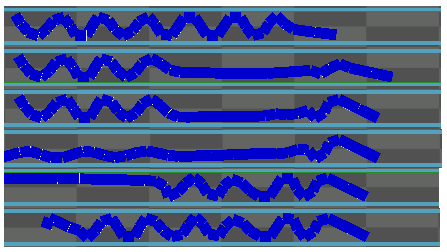
\includegraphics[scale=0.8]{AdaptiveStep.png}
\end{center}
\caption{Adaptive Step Concertina Gait}
\label{adaptive_step}
\end{figure}

1) Rest-State (Initial): Rest-State is the initial fully anchored posture of the snake robot.  This is our initial pose and it acts as a stable platform from which exploratory or probing behaviors can be executed to sense the environment with little chance of slips or vibration due to the multiple anchor contact points.  There is no other action here than to hold the posture that it was already in.  The Rest-State is the initial state and the final state of the concertina gait.

2) Front-Extend:  In the Front-Extend state, the forward segments are gradually transitioned from their initial position to a straight-forward position.  The joints are compliant to the boundaries of the environment to accommodate turns in the pipe.

3) Front-Anchor:  The Front-Anchor state takes the extended portion of the snake and attempts to establish an anchor to the pipe as far forward as possible.  The locomotion distance is maximized the further forward the front anchor is.

4) Back-Extend:  The Back-Extend state follows a successful Front-Anchor event.  All anchors established in the back segments are gradually extended until they are straight.  Again, the joints are compliant so that they can conform to the walls of the environment.

5) Back-Anchor:  The Back-Anchor state involves establishing multiple anchors with the remainder of the body segments.

6) Rest-State (Final):  Upon conclusion of the Back-Anchor state, a single step of the adaptive concertina gait is complete and the snake is now in the Rest-State.  From here we can do probing of the environment or perform another step forward.

A successful transition through all the states results in a single step.  Multiple steps are used to travel through the environment.  We describe no steering mechanism for this locomotion gait because the robot has no means to sense the environment in front of it.  However, the robot’s compliant posture will adapt to any junctions or pipe curvature and follow it.

We now describe the implementation of each of these states and their composition of behaviors.



\subsection{Front-Extend}

%GRAPHIC
%Merge(
%FrontExtend ← HoldSlideTransition ← Transition,
%HoldPosition
%)
\begin{figure}
\begin{center}
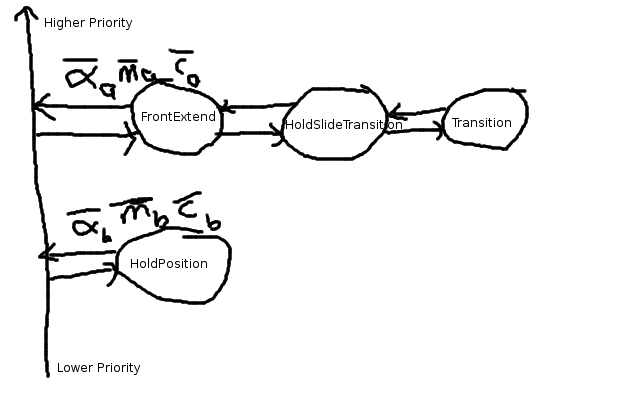
\includegraphics[scale=0.5]{2_adaptive_1.png}
\end{center}
\caption{Front-Extend behavior assembly.}
\label{adaptive1}
\end{figure}

%Convergence merge of 0.0 extension and anchored state.  Precedence merge of FrontExetend and HoldPosition.  HoldPosition holds back half while FrontExtend controls front.  Passes extended state to HoldSlideTransition.  This manages convergence merge and slide with a Transition behavior to handle each step. 

From the fully anchored Rest-State stage, the goal of the Front-Extend stage is to release the front anchors and stretch the front half of the snake as far forward as possible without compromising the rear anchors.  The further forward we can extend, the further the snake can travel in a single step.

If the extended snake arm makes a lateral impact, the walls will guide the movement of the snake but not otherwise hinder the behavior.  In the event of an actual obstruction, the tip’s movement will stop.  We are able to track whether the position of the tip hasn’t moved overtime and are able to set a flag to abort the behavior at the current posture.

Its implementation consists of 4 behaviors arranged as shown in Figure \ref{adaptive1}.  We explain each behavior's functionality.

\textbf{HoldPosition:} The purpose of this behavior is to output the same joint commands indefinitely.  It is instantiated with a vector of joint commands, and it continues to output these joint commands until termination.  In this case, it is instantiated with the entire initial anchored posture of the snake from Rest-State and continues to output this posture.  The behavior’s output is gradually subsumed by the growth of the FrontExtend behavior in a precedence merge.  HoldPosition is placed 2nd in the behavior ordering at the root level for this reason.

\textbf{Transition:} This behavior’s purpose is to take an initial and final pose and interpolate a transition between the two, outputting the intermediate postures incrementally.  The number of interpolated steps used to transition between the poses is set by the parent behavior.  It is often a function of how much difference there is in the initial and final poses.  The clock-rate is dependent on the parent behaviors. Once it reaches the final pose, it returns a flag and continues to output the goal pose indefinitely until reset or deleted.  Here it is instantiated by the HoldSlideTransition behavior and reset each time it needs to make a new move command.

\textbf{HoldSlideTransition:} This behavior was first mentioned in section \ref{sec:merge} and implements the equation \ref{equ:slide}.  Its role is to use a convergence merge to transition from one posture to another.  The convergence parameter $c$ is incremented over time to slide the convergence from the front to the back of the snake, to smoothly transition from the fully-anchored posture to the back-anchored and front-extended posture.

For each change in $c$, the Transition behavior is set up to interpolate smooth motion between the two postures.  Once the Transition behavior completes, $c$ is incremented and Transition is reset to the new initial and final postures.  $c$ is changed from 8 to 20 while using the joint numbers as the indices in the convergence merge equation shown in X, assuming that the joint numbering starts at 0 at the front tip.  An example of the HoldSlideTransition behavior in action is shown in Figure \ref{merging3}.

\textbf{FrontExtend:}  Finally, the FrontExtend behavior creates HoldSlideTransition as a child behavior and gives it its initial and final posture.  It passes through the output of HoldSlideTransition.  It also monitors the pose of the snake tip to see if any obstructions are encountered.  If the pose remains stationary for a period of time, an obstruction is declared and the behavior is halted.  The behavior returns a collision flag.

\subsection{Front-Anchor}

\begin{figure}
\begin{center}
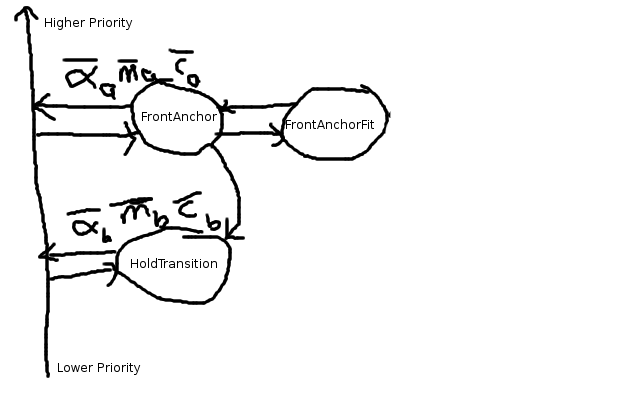
\includegraphics[scale=0.5]{2_adaptive_2.png}
\end{center}
\caption{Front-Anchor behavior assembly.}
\label{adaptive2}
\end{figure}

%GRAPHIC
%Merge(
%FrontAnchor -> FrontAnchorFit, 
%    |
%   V
%HoldTransition
%)

Once the front-half of the snake has been extended by the Front-Extend stage, the next step is to place the first anchor using the already extended segments.  The complete posture of the snake is submitted to a HoldTransition behavior while the front half of the posture is modified by the FrontAnchorFit behavior.

This stage attempts to create a 3-point anchor that is created with the previously extended segments.  The anchor is rooted at an internal joint starting from the merge joint 7 giving 8 segments with which to create the anchor.  In the event that not enough segments are available to create the full anchor, the anchoring process is restarted with +2 more segments by moving the root inward by 2 joints.  

On successful completion of the 3-point anchor with the available segments, a test is performed to see if the anchor is secure, called a jerk-test.  This is accomplished by a sudden rotation of four joints adjacent to the merge joint not on the side of the front anchor.  While tracking the position of the anchor segments, if the anchored portion of the snake moves appreciably from the jerk-test, the anchor is deemed insecure, and the anchoring process is restarted with 2 more segments.

Whenever the merge joint is moved inwards, this also results in the contact positions of the anchor points moving inward as well.  This can be useful for changing the anchor locations if no stable purchase is found, but also reduces the step distance of the gait by reducing the extension length.

The composition of the behaviors is shown in Figure \ref{adaptive2} and described as follows:

\textbf{HoldTransition:}
This behavior is originally initialized with the complete posture of the snake at the outcome of the Front-Extend stage.  The front portion is laterally modified by the FrontAnchor behavior whenever new changes are required to the front anchor shape.  The behavior is stepped and drives the robot joints for smooth transitions.

Though the FrontAnchor behavior has priority over the HoldTransition behavior, FrontAnchor almost never drives an output but instead laterally modifies the HoldTransition behavior.  Therefore, the HoldTransition behavior is the primary driver of the snake robot.

\textbf{FrontAnchor:}
This behavior has complete responsibility for the entire anchoring and testing process.  It creates a 3-point anchor for static stability instead of the 2-point anchors previously described in section 2.1.  This is because this will be the only anchor to the environment in the next stage.  Complete secureness is required to avoid any slip conditions.

A 3-point anchor is created with a cosine curve of period 2.5pi shown in Figure \ref{frontanchor1}.  The FrontAnchor behavior gradually increases the amplitude of this curve.  As the amplitude increases, more and more segments are required to complete the fit.  Should the curve be longer than the available number of segments, the anchoring process is restarted with the merge joint moved back 2 joints.

The anchoring process is halted after search algorithm 2 completes.  The behavior then performs a jerk-test to determine if the anchor points are secure.  If k’th joint is the merge joint, then the joints [k+1,k+4] are rapidly changed in the following sequence:  [(0,0,0,0), (-60,-60,-60,-60), (0,0,0,0), (60,60,60,60)].  These joints are directly controlled by the FrontAnchor behavior to create sudden motion and override the parallel HoldTransition behavior that normally performs smooth motion.

A secure anchor will register little movement in the anchor segments while an insecure anchor will move a great deal.  This movement is tracked through kinematics and assumes that the back anchors are secure and stable.  Once the deviation in position of the anchor segments is below a certain threshold, than we determine that this is a secure anchor and return success.

\textbf{FrontAnchorFit:} 
This behavior is responsible for computing the curve-fitting process described at the beginning of section 2.  It determines the correct joint orientations for a given curve.  The curve is input by the FrontAnchor behavior and modified accordingly.  The FrontAnchorFit behavior performs an efficient curve-fitting process assuming the curve starts rooted at the merge joint on the behavior boundary shown in Figure \ref{frontanchor1}.

\begin{figure}
\begin{center}
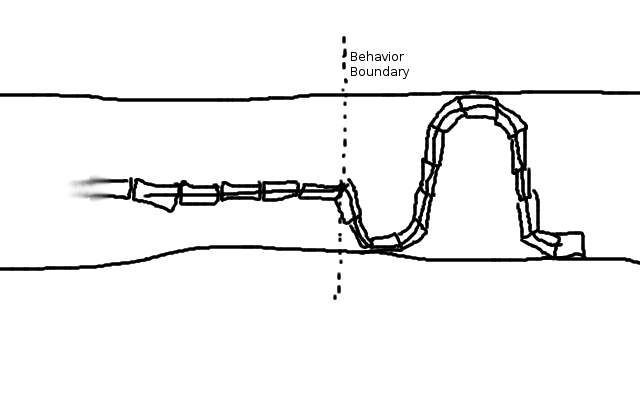
\includegraphics[scale=0.5]{2_frontanchor_1.png}
\end{center}
\caption{Posture that creates a 3-point anchor.}
\label{frontanchor1}
\end{figure}


\subsection{Back-Extend}

\begin{figure}
\begin{center}
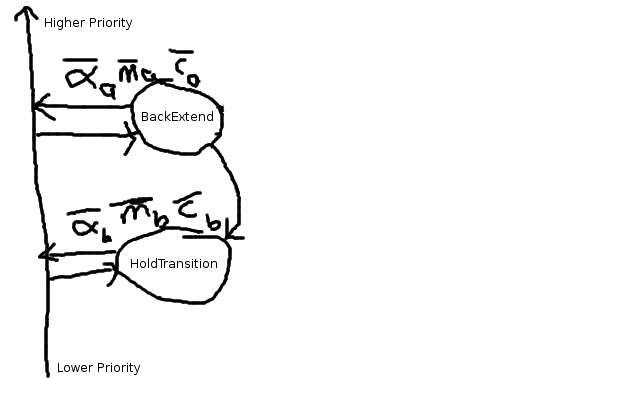
\includegraphics[scale=0.5]{2_adaptive_3.png}
\end{center}
\caption{Back-Extend behavior assembly.}
\label{adaptive3}
\end{figure}

%GRAPHIC
%Merge(
%BackExtend
%    |
%    V
%HoldTransition
%)

After the front anchor has been securely established, the next stage’s role is to remove the back anchors and extend the back half of the body straight.  If the environment prevents the back half from being straight, the joints are compliant to the environment and will extend as far as they are allowed.

The behaviors are shown in Figure \ref{adaptive3} and described as follows:

\textbf{BackExtend:}
This behavior simply takes all the joints on one side of the merge joint behavior boundary and commands their values to be 0.0.  It also sets all of these joints to have low torque to ensure compliant motion.  These values are sent laterally to the HoldTransition behavior.

\textbf{HoldTransition:} 
This behavior is initialized to the posture from the outcome of the Front-Anchor stage.  It receives as input from the FrontExtend behavior, the new straight 0.0 joint positions.  It manages the smooth motion from the back anchored position to the back extended position.


\subsection{Back-Anchor}

\begin{figure}
\begin{center}
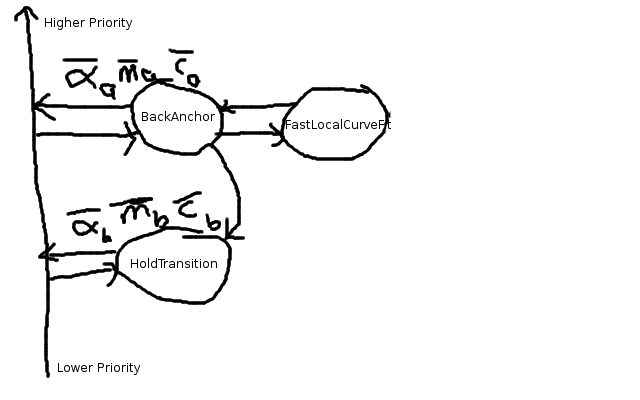
\includegraphics[scale=0.5]{2_adaptive_4.png}
\end{center}
\caption{Back-Anchor behavior assembly.}
\label{adaptive4}
\end{figure}

%GRAPHIC
%Merge(
%BackAnchor -> FastLocalCurveFit, 
%    |
%    V
%HoldTransition
%)

The purpose of this stage is form the 2-point anchors described in section 2.1 with the remaining extended segments of the back half of the snake.  The sine curves are joined together with the front anchor cosine curve to make a continuous splice merge and produce a complete anchored posture of the whole snake.

New pairs of anchor points are created, using one period of a sine curve each, until all of the remaining back segments are used up.  At each anchor pair, we use the adaptive anchoring algorithm 2 to detect contacts.  However, we do not perform a jerk-test like in the Front-Anchor stage because we only have the front anchor as our reference point and no extra joints to perform the jerking motion.  Furthermore, it is not as critical to determine if the back anchors are secure since there are more of them, and we have confidence in the security of our front anchor.


The behaviors are shown in Figure \ref{adaptive4} and described as follows:

\textbf{HoldTransition:} 
This behavior fulfills the same role as all of the other instances.  It takes the initial posture at the outcome of the previous stage and maintains that posture until modified by the primary behavior, BackAnchor.   It manages the smooth transition between postures.

\textbf{BackAnchor:} 
This behavior performs the anchor contact algorithm 2, modifies the curve parameters, and continues to add anchor pairs until it runs out of segments.  It creates the FastLocalCurveFit behavior as a child behavior.

\textbf{FastLocalCurveFit:} 
This behavior parameterizes the curves representing the series of back anchor curves of varying amplitudes.  It is also responsible for efficiently computing the joint positions to fit the snake to the curves.  Furthermore, it accepts compliance in the curve-fitting process between each anchor pair.  That is, at each merge joint between two anchor pairs, compliance is to find the best anchor posture and the posture is saved for the remainder of the stage.


\section{Analysis}


Our theoretical contribution is a quantitative analysis of the trade-space between environmental characteristics, snake robot morphology, and locomotion control parameters.  That is, given a snake robot morphology and control parameters, what types of environments can we successfully explore.  Conversely, given a specific environment, what robot morphology and control parameters are required to successfully explore it.

First we will perform an analysis of the trade-space for forming a 3-point stable anchor in a smooth pipe.  A 3-point anchor is shown in Figure \ref{param_1} and is the minimum number of contact points required to form a stable anchor.  This posture will hold the body of the snake rigid and prevent it from translating or rotating within a threshold of external force and torque.

We will define and quantify the parameters that describe this system: the environment, the robot, and the control.

Our particular environment of a smooth pipe can easily be described with one parameter, the pipe width $W$.

The complete snake robot morphology can be described by 3 parameters: segment width $w$, segment length $l$, and number of segments $n$.

Finally, control of the robot is achieved by fitting the body of the snake onto a curve described by a sinusoid.  The parameters for control are the values of amplitude $A$ and period $P$, where $y = A \cos(\frac{2 \pi x}{P})$.  

\begin{figure}[htb]
\begin{center}
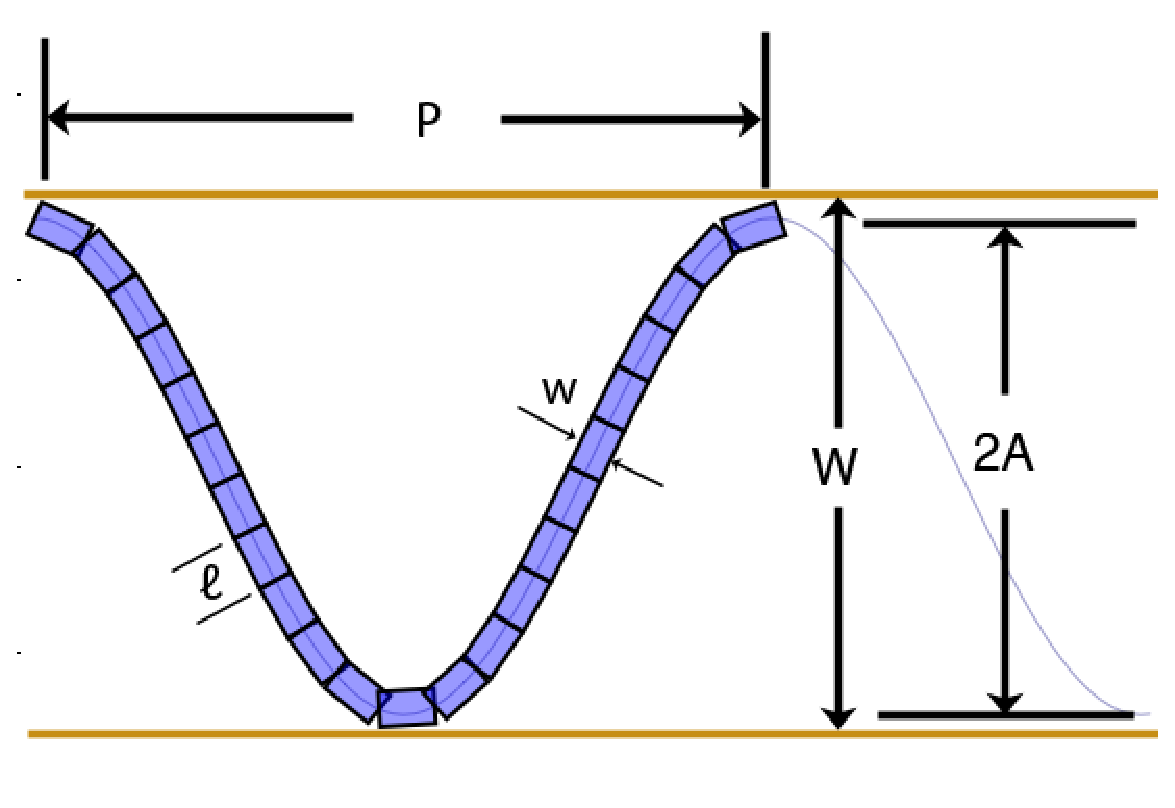
\includegraphics[scale=0.5]{CurveDiagram}
%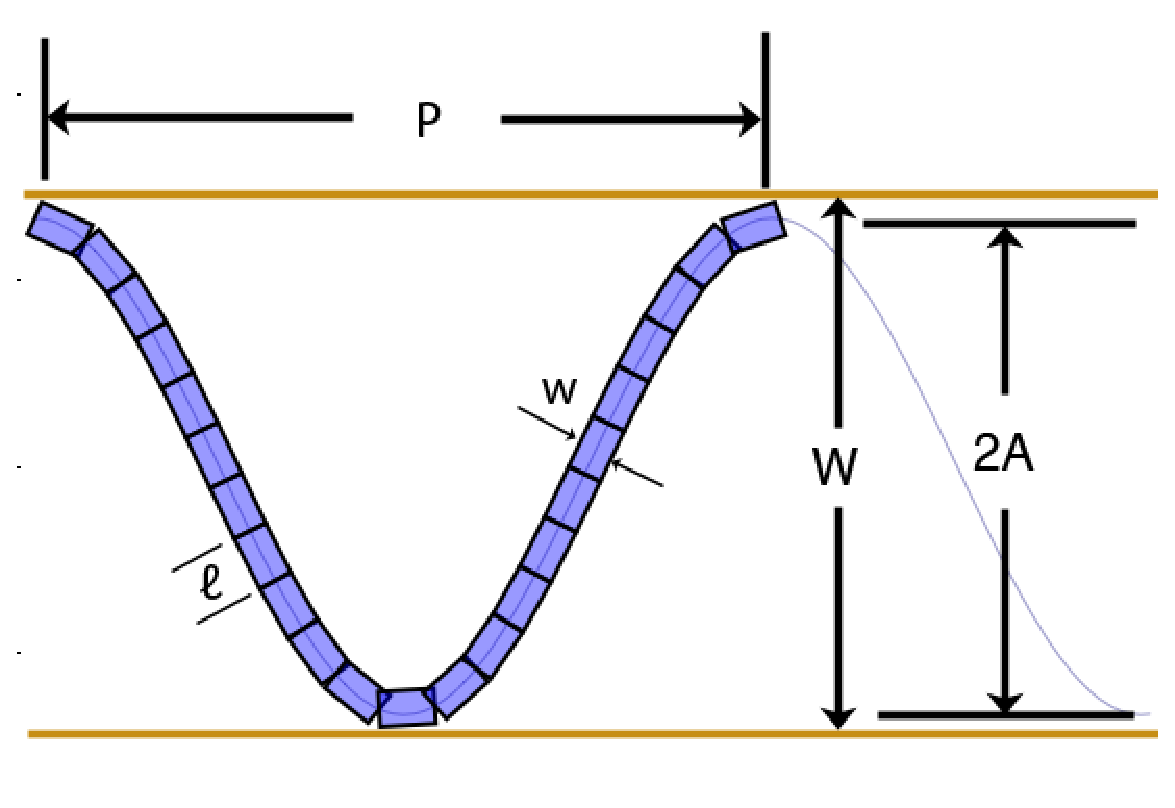
\includegraphics{CurveDiagram}
\end{center}
\caption{Parameterization of 3-point stable anchor in a smooth pipe.}
\label{param_1}
\end{figure}

\subsection{Case: Snake as a Curve}

We first consider the degenerate case where $l = 0$, $w = 0$, and $n = \infty $.  This results in a snake that has no width and an infinite number of joints.  Essentially, the snake body equals the curve equation.  Since $w = 0$, this results in $ 2A = W $.  This is shown Figure \ref{deg_1}.

\begin{figure}[htb]
\begin{center}
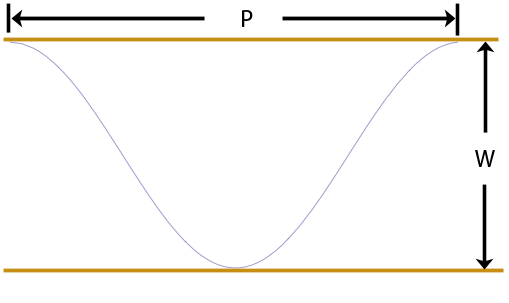
\includegraphics[scale=0.5]{DegenerateCurve}
%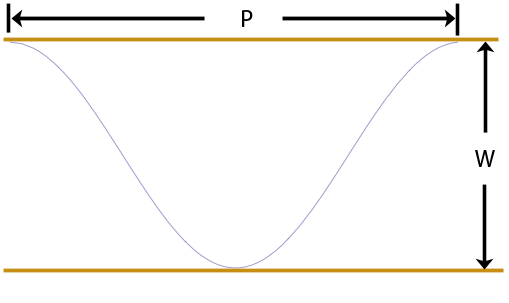
\includegraphics{DegenerateCurve}
\end{center}
\caption{3-point stable anchor with $w = 0$, $l = 0$, and $n = \infty $.}
\label{deg_1}
\end{figure}

We define $L$ to be the total length of the snake which can be computed from the equation of the curve.

\begin{equation}
f(x) =  \frac{W}{2} \cos \left( \frac{2 \pi x}{P} \right) 
\end{equation}

Equation 1 is the equation of the curve with $P$ the period, $W$ the width of the pipe.   We can plug $f(x)$ into the equation for computing arc length shown in Equation 2 and 3:

\begin{equation}
L = \int_{0}^{P} \sqrt{f'(x)^2 + 1} \,\,\, dx
\end{equation}

\begin{equation}
L = \int_{0}^{P} \sqrt{\left( \frac{-W \pi}{P} \sin \left( \frac{2 \pi x}{P} \right)  \right)^2 + 1} \,\,\, dx
\end{equation}

This integration can not be solved analytical and must be solved by plugging in values for $P$ and $W$ and computing $L$ numerically.  In our control methodolgy, $P$ is usually held fixed and the width of the environment is always changing, so $W$ is always varying.  Here we show a plot holding $P$ fixed for various values while changing the value of $W$ in Figure \ref{plot_1}.

\begin{figure}[htb]
\begin{center}
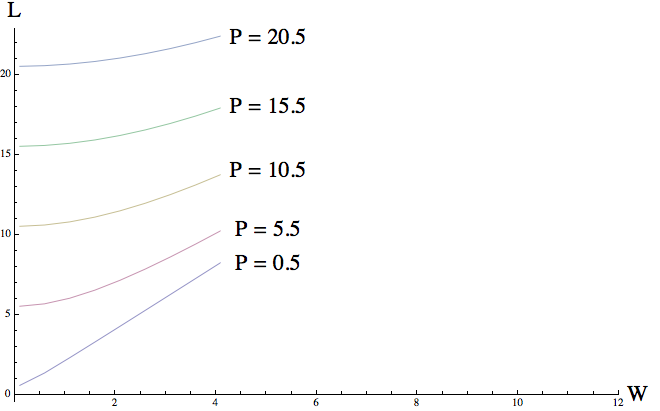
\includegraphics[scale=0.6]{2011_01_23_Plot_DegenerateAnchor}
\end{center}
\caption{Plot of snake arc length $L$ for various values of $W$ and $P$.}
\label{plot_1}
\end{figure}

This plot shows that when pipe width $W \to \infty$, the length $L$ converges to a constant slope of $\frac{dL}{dW} = 2$ and $L = 2W \,, \forall P$ as $W \to \infty$.  This can be seen by approximating the 3-point anchor and cosine curve as a triangle with a base of $P$ and a height of $W$, and the vertices on the anchor points.  Increasing $W$ will achieve the above results.

The difference in $L$ becomes large for different values of $P$ when $W$ is small.  Once $W$ becomes sufficiently large, $W$ dominates and the period becomes less of a factor.   Given that our application involves tight quarters, we are likely to find typical values of $W$ to be small and $P$ will vary depending on the context.

\subsection{Case: Snake with Width}

We now consider the case where $l = 0$, $n = \infty$, but $w > 0$.   This in effect creates a continuous snake robot with infinite joints but has a thickness to it.  To determine the total length of the snake given a pipe width $W$, a control period $P$, and a segment width of $w$, we first determine the equation of the curve:

\begin{equation}
f(x) =  \frac{W-w}{2} \cos \left( \frac{2 \pi x}{P} \right) 
\end{equation}

Since the snake centers its body on the curve, it has space of $\frac{w}{2}$ on either side of it.  We start the cosine amplitude at $\frac{W}{2}$ and substract $\frac{w}{2}$ as the width of the snake increases.  This results in equation 4.

If we plug the $f(x)$ into the arc length equation, we get the snake length for given $W$, $P$, and $w$:

\begin{equation}
L = \int_{0}^{P} \sqrt{\left( \frac{-(W-w) \pi}{P} \sin \left( \frac{2 \pi x}{P} \right)  \right)^2 + 1} \,\,\, dx
\end{equation}

Holding $P = 1$, and increasing the pipe width $W$ for different values of $w$, we get the following plot shown in Figure \ref{plot_2}.  This plot captures the intuition that a snake robot is not able to explore a pipe that is thinner than the robot's body width.  However, once you enter a pipe where $W > w$, the plot takes on the same curve as Figure \ref{plot_1}.  For large enough $W$,  $L = 2(W-w)$ and $\frac{dL}{dW} = 2$.

\begin{figure}[htb]
\begin{center}
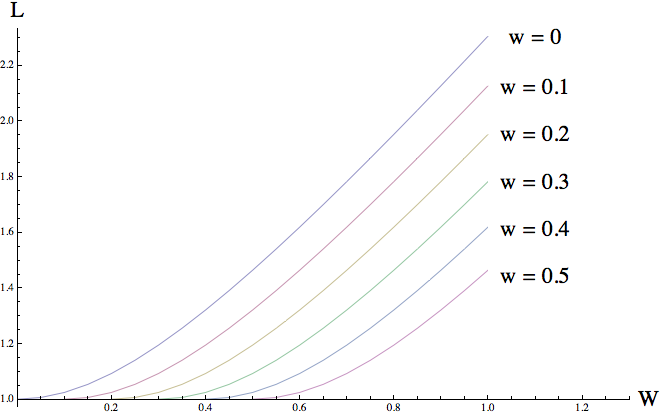
\includegraphics[scale=0.6]{2011_01_24_Plot_WidthAnchor}
\end{center}
\caption{Plot of snake length $L$ while $P=1$, for various values of $W$ and $w$.}
\label{plot_2}
\end{figure}

\subsection{Case: Snake with Segments}

We now consider the case where the robot composed of discrete segments of a given length $l$.  Up until now, we have represented the snake as a curve function.  However, with segments, the robot needs to fit its body to be placed on the curve.   Our current approach assumes a monotonic curve in the x-direction and the joint axes are placed directly on the curve.  In this example, we assume that curve fitting is perfect and unique.

Again we look at the 3-point anchor situation determine how the length of the snake changes with different parameters.  Instead of length though, we are computing the number of required snake segments.

There are two approaches.  The first is to examine the situation analytically, deriving an equation for the number of segments given period $P$, pipe width $W$, and segment length $l$.  The second is to run an algorithm that performs the curve fitting given a curve and lets us determine the required number of segments.  We do both.

Analytically, we can easily compute an upper bound for the number of segments.  If we have already calculated $L$, we can determine that we will need at most $n$ segments shown in equation 6.

\begin{equation}
n = \left \lceil \frac{L}{l} \right \rceil
\end{equation}

At most $n$ segments will be required in the worst case where the segments lay directly on the curve.  However, in most cases, the segments will be cutting corners to put both ends on top of the curve.  This will result in the required number of segments being less than the worst case.

Algorithmically, we can determine the actual number of segments required for a given configuration.  Given a monotonic curve $\gamma$, draw a circle $c$ at the start of the curve with radius $l$ and origin $o$.  Take all the intersection points between $c$ and $\gamma$. Take only the intersection points where $p_x > o_x$.  Select $p$ with the smallest $x$ value.  Place a segment going from $o$ to $p$.  Set $o = p$ and repeat until there is no more curve.  This looks like the following in Figure \ref{plot_3}.

\begin{figure}[htb]
\begin{center}
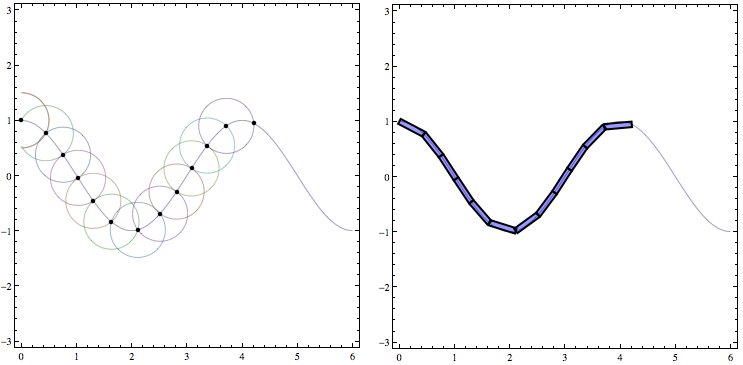
\includegraphics[scale=0.6]{2011_01_28_FitAlgorithm_Segs}
\end{center}
\caption{Intersecting circles along the line of the curve.  Demonstration of curve fitting algorithm.}
\label{plot_3}
\end{figure}




\section{Experimental Results}

We put our results here.






\chapter{Motion Estimation from Proprioception}
\section{Problem}


Now that our snake robot is capable of moving through the environment with the adaptive concertina gait behavior, we need some way of estimating how far it is moving and in which direction.

As we established earlier, we have no external sensors because we assume their failure from environmental conditions.  We cannot rely on GPS since it is not effective underground or in pipes.  We do not have wheeled shaft encoders since we have no wheels and do not expect to always travel through flat terrain.  Finally, although it may indeed help, we cannot expect to make use of an inertial navigation system since they are bulky and expensive.  Furthermore, we have not performed experiments to determine if they are capable of handling the high amount of rotation of each of the snake body segments during locomotion.

In absence of a global positioning or odometry, we need some form of alternative motion estimation. Knowing where the robot is located is the basic building block of creating a map.  We focus on the problem of finding the relative geometric transform between the two poses at the beginning and end of one step of the adaptive concertina gait. 

Our proprioceptive approach achieves motion estimation by anchoring multiple points of the body with the environment and kinematically tracking the change in distance between the immobilized parts as the snake contracts and extends.  This gives us a motion estimation method that only depends on the joint sensors.  We show the effectiveness in a series of experiments.
 

\section{Immobilizing the Anchors}

\label{sec:anchors}

%-Immobilize anchors to create global references
%-Conditions when immobility or anchor slip occurs
%-How to know when immobilized (heuristics)

A fundamental property of the adaptive concertina gait is that it creates anchors to the surrounding environment.  Our goal is to exploit this property to estimate our motion through the environment.  In order to do this, we need to ensure that our anchors remain an accurate frame of reference to the global environment.

The primary goal of our previous work on maintaining smooth and stable motion of the snake in Chapter 2 was to prevent any sort of anchor slip that may harm our reference frame to the global environment.  It is critical that our anchors remain firmly immobilized with respect to the environment to ensure accurate measurement of motion.

Though we are not able to localize the exact contact point of the anchor with the environment, we can assume that the segments comprising the anchoring curve are themselves immobilized and mechanically isolated by virtue of their static contacts with the environment.  We use these isolated bodies as immobilized references to the global environment.

Whether or not we consider the use of a body segment as a reference is determined by our work in Section 2.8.  That is, if the joints in the local neighborhood of a segment are locally stable and the behavior's control bit for the attached joint is 0, we assume this segment is immobilized.  We can use immobilized segments as reference points to the global frame.

We call the monitoring of local joint variances as local stability and the output of the control masks as prescriptive stability.  Though a body segment may be locally stable, it does not mean it is immobile.  If we also include prescriptive stability, the behavior's prediction of what joints should be moving and what should not, then we greatly decrease the chances that we will use a slipping anchor as a reference.

If any point the anchor should slip while, our assumption that a body segment is immobilized is violated and could lead to accumulated errors in our motion technique.  Therefore, it is critical that we analyze and mitigate all the possible failure modes for anchoring.

We are generally able to classify the types of anchoring and reference errors we encounter during both static and locomotive anchoring.  For each, we are forced to either avoid the condition from occurring or detect and correct it. We list the failure modes and explain our mitigation strategy for each.

The \emph{floating reference} occurs when a locally stable segment is made a reference, but it is not part of an anchor. This was particularly troublesome in our early implementations, but we are able to largely avoid this failure mode by having the behaviors explicitly classifying which joints are part of an anchor. The other possibility for a floating anchor would be if an anchoring behavior erroneously reports success in establishing an anchor in free space. This was largely avoided by adding the more careful anchoring process in Section 2.2 that detects impacts to the walls and follows up by doing a jerk test to test whether the anchor is secure.

A \emph{weak contact} occurs when the anchor the reference segment is on has an insecure anchor. This usually happens if an anchor is placed within a pipe junction or if one of the anchors of the Back-Anchor is insecure.  The Back-Anchor case is more likely since they are not jerk-tested.  Weak contacts usually do not display local instability since the physical contact stabilizes the local joints but does not immobilize them.  If it is available, we can use negative prescriptive stability from the behavior to minimize this failure but often occurs in prescriptively stable areas.  There is nothing we can do to prevent this error from being added to the pose estimation besides detecting it.  Luckily, a weak contact does not move much.  Its error is bounded.

\emph{Buckling} occurs when the anchored joints are frozen in a non-optimal position and external stresses put excessive torque on one or more joints that forces the anchor into a reconfigured position. This is similar to mechanical buckling of structural members under compression.  In this case, it is for an articulated system attempting to hold a rigid pose. Buckling is easily detectable by tripping our local stability conditions and will quickly remove the references and reuse them once the joints have settled down. We have also reduced this occurrence by having our anchoring behaviors search for non-deforming anchors as a natural by-product of algorithm 2.

\emph{Impulses} occur when the snake robot experiences a sudden collision or a buckling has occurred somewhere else in the robot. Usually this is not a fatal error and the robot will quickly return to its stable pose. However it can trip up the variance calculations and deactivate all the references we have leaving us with none. Recovery is achieved by resurrecting the last best reference, and assuming it is in the same pose.  We show how to do this in the next section.

\emph{Funnel anchoring} occurs when a secure anchor is established between a pair of walls that are monotonically increasing in width. If the anchor receives a force that pushes it towards the direction of increasing width, its anchor can become permanently loose. This is especially problematic in cases of irregular environments where there are many possibilities for this to occur in local conditions. We currently do not have a solution for this yet.

Finally there is a class of \emph{whole body slip} that is completely undetectable with only joint positions. That is, the whole body could be slipping through an environment such as a straight and featureless pipe without causing any joint variance at all. This would only occur if the ground was exceptionally slippery and able to use the robot's momentum to move it large distances or if the robot was on a slope and gravity was exerting a global force. We avoid this error by limiting the environments we explore. Other environments may require extra sensor instrumentation such as accelerometers to detect this failure mode.

Rotational error is the dominant form of error we encounter because, unlike a traditional robot with a stable frame of reference on its chassis, every reference point in the snake robot's body is constantly in rotational motion. Any form of disturbance of a reference node will manifest itself with a rotational error that will propagate through kinematic computations of new reference nodes. Translational error occurs primarily by anchor slip.  Rotational error is easier to correct in our later localization process in Chapter 5.

\section{Tracking Motion}

%-What a reference is
%-each active reference can be used to compute the pose of the snake at that given time
%-active references may disagree with each other
%-take current oldest active reference to compute current pose
%-How to create new references (kinematic computation)
%-When to deactivate references (violation of local/pre stability)
%-Loss of all references recovery

In order to track motion through the environment, we need to establish our mathematical framework for defining the relative position of things between the robot and the environment.  We then define the concept of a \emph{reference pose} to track the position of the environment while the snake is in motion.

\subsection{Pose and Coordinate Frames}

\begin{figure}
\begin{center}
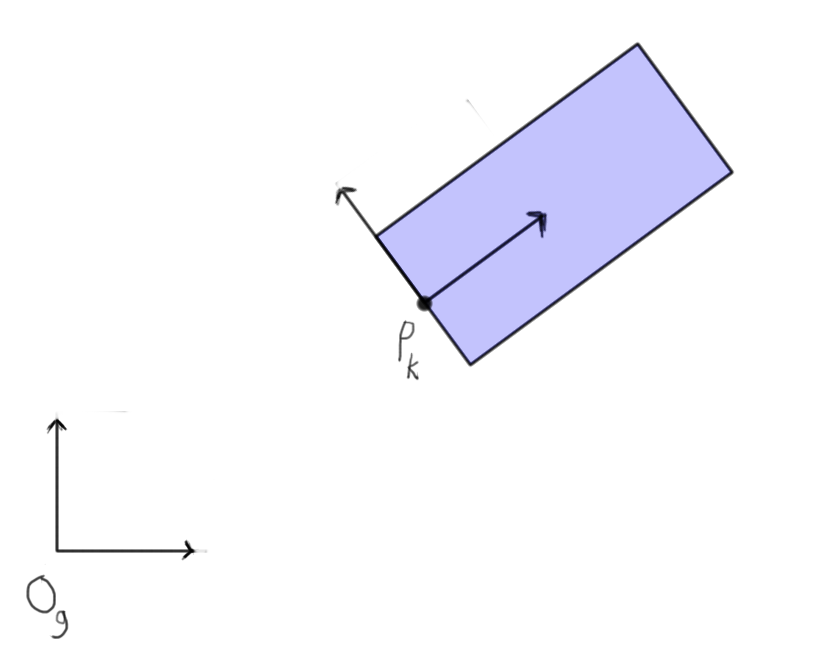
\includegraphics[scale=0.5]{3_pose_frame1.png}
\end{center}
\caption{Pose of rigid body with respect to global frame.}
\label{fig:pose_frame1}
\end{figure}

A pose $P$ defines the position and orientation of a rigid body in a 2D plane.  Each pose is defined with respect to a coordinate frame $O$ using 3 values: $(x,y,\theta)$.  A coordinate frame is either affixed in the global environment or affixed to a rigid body on the snake.  An example of the global frame $O_g$ and a pose $P_k$ are shown in Figure \ref{fig:pose_frame1}.

By convention, we will specify in the superscript which coordinate frame a pose $k$ is defined with respect to.  For the global frame, the pose is written as $P_k^g$.  If the pose is with respect to some other coordinate frame $O_a$, the pose is written as $P_k^a$.  If the superscript is omitted, we assume the global frame.

\begin{figure}
\begin{center}
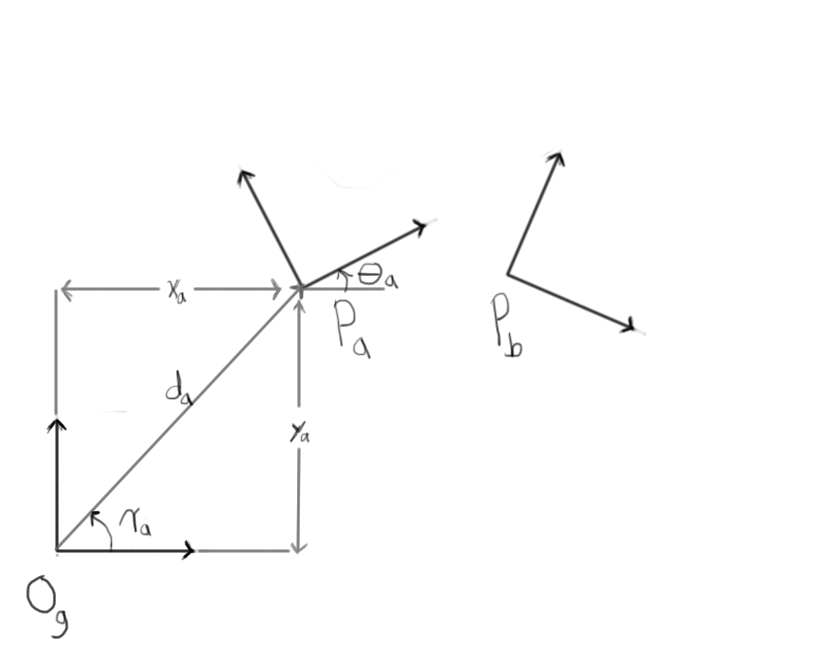
\includegraphics[scale=0.5]{3_pose_frame2.png}
\end{center}
\caption{Pose of A and B with respect to global frame.}
\label{fig:pose_frame2}
\end{figure}

In a robot system with multiple rigid bodies, we will have a coordinate frame for each body.  Often times, we wish to transform poses between coordinate frames.  To do this, we first need to define the relationship between coordinate frames, specified by the pose of their origins.  In the global frame $O_g$, the pose of the origin $O_g$ is $P_g = (0,0,0)$.  For two example coordinate frames attached to rigid bodies, we define the pose of origin $O_a$ to be $P_a = (x_a, y_a, \theta_a)$ and the pose of origin $O_b$ to be $P_b = (x_b, y_b, \theta_b)$ as shown in Figure \ref{fig:pose_frame2}.

Suppose we wanted to compute pose $b$ with respect to frame $O_a$.  That is, we wish to find $P_b^a$ and we are given $P_a^g$ and $P_b^g$.  First we focus on finding the Cartesian component of the pose, point $p_b^a = (x_b^a, y_b^a)$.  We compute the angle portion $\theta_b^a$ separately.  From Figure \ref{fig:pose_frame2}, we define the following:
\begin{equation}
\label{equ:coord1}
R_a =
\begin{bmatrix}
cos(\theta_a) & sin(\theta_a) \\
-sin(\theta_a) & cos(\theta_a)
\end{bmatrix}
\end{equation}

This is the rotation matrix for the difference in orientation between the global frame $O_g$ and local frame $O_a$.
\begin{equation}
\label{equ:coord2}
d_a = \sqrt{(x_a)^2 + (y_a)^2} 
\end{equation}

This is the Cartesian distance from the global frame's origin to the local frame's origin.
\begin{equation}
\cos(\gamma_a) = \frac{(x_a,y_a) \cdot (1,0)}{|(x_a, y_a)| |1|} = \frac{x_a}{d_a} 
\end{equation}
\begin{equation}
\label{equ:coord3}
\gamma_a = s \cdot \arccos \left( \frac{x_a}{d_a} \right) 
\quad
\left\{ 
  \begin{array}{l l}
    s = 1 & \quad \text{if $y_a \geq 0$}\\
    s = -1 & \quad \text{if $y_a < 0$}
  \end{array} \right.
\end{equation}

$\gamma_a$ is the angle of the vector from the global origin to the local frame origin.  The sign of $\gamma_a$ is determined to be negative if $y_a < 0$.  Otherwise, $\gamma_a$ is positive.  This value corresponds to the angle shown in Figure \ref{fig:pose_frame2}.
\begin{equation}
\label{equ:coord4}
G_a = 
\begin{bmatrix}
cos(\gamma_a) & sin(\gamma_a) \\
-sin(\gamma_a) & cos(\gamma_a)
\end{bmatrix}
\end{equation}

$G_a$ is the rotation matrix to rotate the local frame's origin onto the x-axis of the global frame.

To find $p_b^a$ in frame $O_a$ from $p_b^g$ in $O_g$, we compute:
\begin{equation}
\label{equ:g_to_c_cart}
p_b^a =
\begin{bmatrix}
x_b^a \\
y_b^a \\
\end{bmatrix}
 = R_a {G_a}^{\mathbf{T}} \left(G_a p_b^g 
-
\begin{bmatrix}
d_a \\
0
\end{bmatrix}
\right)
\end{equation}

To find the converse, $p_b^g$ from $p_b^a$, we do the following:
\begin{equation}
\label{equ:c_to_g_cart}
p_b^g =
\begin{bmatrix}
x_b^g \\
y_b^g \\
\end{bmatrix}
 = {G_a}^{\mathbf{T}} \left(
\begin{bmatrix}
d_a \\
0
\end{bmatrix}
+ G_a {R_a}^{\mathbf{T}} p_b^a \right)
\end{equation}

This approach performs a sequence of rotations to separate translation and rotation of the pose when converting between frames.  To compute the angle portion of the pose, we perform the rotation sequence by addition and subtraction of angles.  Following the sequence, we get the following: 
\begin{equation*}
\theta^a_b = \theta_b^g + \gamma_a - \gamma_a - \theta_a
\end{equation*}
This reduces to:
\begin{equation}
\label{equ:g_to_c_ori}
\theta^a_b = \theta_b^g - \theta_a
\end{equation}

The converse is achieved similarly using Equation \ref{equ:c_to_g_cart} and the following rotation sequence:
\begin{equation*}
\theta_b^g = \theta_b^a + \theta_a + \gamma_a - \gamma_a 
\end{equation*}
\begin{equation}
\label{equ:c_to_g_ori}
\theta_b^g = \theta_b^a + \theta_a
\end{equation}

The final result for the pose computation is to put the Cartesian and angular components together.
\begin{equation}
P_b^a =
\begin{bmatrix}
x_b^a \\
y_b^a \\
\theta_b^a 
\end{bmatrix}
\quad
\left\{ 
  \begin{array}{l l}
    x_b^a,y_b^a & \quad \text{from Equation \ref{equ:g_to_c_cart}}\\
    \theta_b^a & \quad \text{from Equation \ref{equ:g_to_c_ori}}
  \end{array} \right.
\end{equation}
And the converse is:
\begin{equation}
P_b^g =
\begin{bmatrix}
x_b^g \\
y_b^g \\
\theta_b^g 
\end{bmatrix}
\quad
\left\{ 
  \begin{array}{l l}
    x_b^g,y_b^g & \quad \text{from Equation \ref{equ:c_to_g_cart}}\\
    \theta_b^g & \quad \text{from Equation \ref{equ:c_to_g_ori}}
  \end{array} \right.
\end{equation}


Now that we have established the mathematical framework for relating the pose of the rigid bodies to the environment and each other, we describe our concept of reference poses to track motion in the environment.


\subsection{Reference Poses}

A reference pose is the position and orientation of a rigid body segment that has been immobilized with respect to the global frame.  A reference pose is valuable because it gives a fixed reference point to the global environment and allows us to track the motion of the rest of the robot.   Special care must be taken to ensure that when using a reference pose, the rigid body it's attached to is truly immobilized.

A reference pose is either active or inactive.  A reference is active once it is created as a result of its rigid body becoming immobilized.  We assess whether a reference pose is to be created by checking if it satisfies both our predictive stability and local stability conditions.  We discussed predictive and local stability in section \ref{sec:stability}, where predictive stability is the output of the behavior's control masks and local stability is the result of monitoring local joint variances.  Once the reference pose violates either of these conditions, it becomes inactive.

To deactivate a reference pose, if a reference violates either of the stability conditions and it was previously active, we flip a bit to signal it as inactive.  Afterwards, we can create a new reference pose on this rigid body once it satisfies the stability conditions again.

To create a new reference pose, its associated rigid body must first have been inactive.  Secondly, it must satisfy both prescriptive and local stability conditions.  Once the following conditions have been met, the new pose is computed kinematically with respect to another currently active reference pose.  If the pre-existing reference pose is correct, the kinematic computation of the new reference pose will be correct for its true position and orientation in the global environment.

Given the arrangement of rigid bodies and their attached coordinate frames shown in Figure \ref{frames2}, we need the kinematic equations for computing the pose of a rigid body given its neighbor's pose.  That is, if we already have an active reference pose, we wish to compute the pose of neighboring reference in the global frame using only the joint angles from the robot's posture.  To compute $P_{k+1}$ if we are given $P_k$, we do the following:
\begin{equation}
\begin{array}{l}
\displaystyle x_{k+1} = x_k + l \cos(\theta_k) \\
\displaystyle y_{k+1} = y_k + l \sin(\theta_k) \\
\displaystyle \theta_{k+1} = \theta_k - \phi_{k+1}
\end{array}
\label{kinem1}
\end{equation}
For the opposite direction, to compute $P_{k+1}$ given $P_k$, we do the following:
\begin{equation}
\begin{array}{l}
\displaystyle \theta_k = \theta_{k+1} + \phi_k \\
\displaystyle x_k = x_{k+1} - l \cos(\theta_k) \\ 
\displaystyle y_k = y_{k+1} - l \sin(\theta_k)
\end{array}
\label{kinem2}
\end{equation}
If we use the equations iteratively, we can compute the pose of a rigid body segment given the pose of any other segment. 

The algorithmic process for creating and deactivating reference poses is shown in Algorithm \ref{alg:reference}, where $N$ is the number of rigid body segments in the snake from which to create reference poses.  The implementation of the function for the kinematic computation of new reference poses is shown in Algorithm \ref{alg:kinematic}.


\begin{figure}
\begin{center}
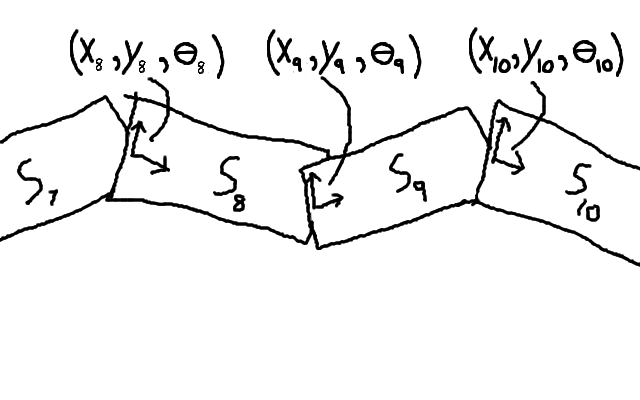
\includegraphics[scale=0.5]{3_frames_2.png}
\end{center}
\caption{Local coordinate frames attached to segments and described by reference poses.}
\label{frames2}
\end{figure}


\begin{algorithm}
\caption{Reference Pose Creation and Deactivation}          % give the algorithm a caption
\label{alg:reference}
\begin{algorithmic}

\State $N \Leftarrow 40$
\State $activeMask \Leftarrow $ array of size $N$ initialized to $0$
\State $activeRefPoses \Leftarrow $ array of size $N$ initialized to $\varnothing$
\State $preStabMask \Leftarrow \mathrm{behaviorControlOutput}()$
\State $locStabMask \Leftarrow \mathrm{stabilityCompute()}$
\For{$i = 0 \to N$} 
\If  {$preStabMask[i] \And locStabMask[i]$}
\If    {$!activeMask[i]$}
\State      $activeRefPoses[i] \Leftarrow \mathrm{computeRefPose}(i)$
\State      $activeMask[i] \Leftarrow 1$
\EndIf
\ElsIf {$activeMask[i]$}
\State    $activeRefPoses[i] \Leftarrow \varnothing$
\State    $activeMask[i] \Leftarrow 0$
\EndIf
\EndFor

\end{algorithmic}
\end{algorithm}

\begin{algorithm}
\caption{\emph{computeRefPose(i)}: Kinematics for Computing Reference Pose}
\label{alg:kinematic}
\begin{algorithmic}

\State $N \Leftarrow 40$
\State $\bar{\phi} \Leftarrow $ array of current joint angles 
\State $i \Leftarrow $ target new reference pose index
\State $j \Leftarrow $ index of nearest active reference pose to $i$

\State $k = j$
\State $(x_k, y_k, \theta_k) \Leftarrow (x_j, y_j, \theta_j)$  \Comment{pose of active reference $j$}

\If {$i > j$}
\While {$k < i$}

\State $x_{k+1} = x_k + l \cos(\theta_k)$
\State $y_{k+1} = y_k + l \sin(\theta_k)$
\State $\theta_{k+1} = \theta_k - \phi_{k+1}$
\State $k = k + 1$
\EndWhile

\ElsIf {$i < j$}
\While {$k > i$}

\State $\theta_{k-1} = \theta_k + \phi_{k-1}$
\State $x_{k-1} = x_k - l \cos(\theta_{k-1})$
\State $y_{k-1} = y_k - l \sin(\theta_{k-1})$
\State $k = k - 1$

\EndWhile
\EndIf

\State $(x_i, y_i, \theta_i) \Leftarrow (x_k, y_k, \theta_k)$ \Comment{new pose for active reference $i$}

\end{algorithmic}
\end{algorithm}

This algorithm assumes that an active reference pose always exists.  There are two special cases when no reference poses are currently active.   In the first case, the algorithm is initializing and no reference poses have been created yet.  In the second case, all of the reference poses violate the stability condition and all have been deactivated.  These special cases are not shown in the algorithms, but we explain are approach here.

For the first case, when we initialize, the first reference pose is set to $(0,0,0)$.  This becomes the origin of the global frame centered at the robot's starting position in the environment.  From this first initial reference pose, all new reference poses are derived. 

In the second case, no active reference poses are available since no stability conditions have been satisfied.  The robot has effectively lost track of its position in the environment.  In the event that a new reference pose needs to be created, there is no parent pose from which to kinematically compute.  Instead, from the last used inactive reference poses, we select the reference that was contiguously active the longest and use this as the parent pose to compute the new active reference pose.  The reasoning behind this is that a long-lived reference pose is more likely to be correct than a short-lived reference pose due to the sometimes intermittent nature of reference poses.  This last best reference pose approach is very effective in practice.  

So long as the active reference poses satisfy the assumption of no-slip anchors and there always being at least one active reference, the tracking of the robot's trajectory through the environment is correct.  Violations of these assumptions introduce error into the motion estimation.

\section{Robot-Centered Coordinate Frame}

%-N possible local coordinate systems in snake
%-none are very good to represent pose of snake because of the high variance in orientation.  Try to relate two poses to each other, orientation has almost no correlation
%-orientation is also primary source of error
%-prefer a coordinate system that represents the gross posture and pose of snake.  COM can sometimes be out of body
%-GPAC pose proposed.

\label{sec:GPAC}

Though we now have a local coordinate frame for each segment in the snake, we need a coordinate frame that represents the mobile robot body as a whole.  In traditional mobile robots, we usually have a large rigid body chassis with high inertia that is suitable for defining the position and orientation of the robot.  In a snake robot, there are multiple rigid bodies, all of which are small in mass, small in inertia, and poor at defining the overall snake's position and orientation.  While the snake is executing its locomotion, the body segments are undulating and rapidly changing orientation, making dubious their use as an indication of heading.

In the wake of these phenomena, we found the need to create a dynamically generated coordinate frame that best represents the position and orientation of the snake robot's posture as a whole.  We cannot use the center of mass of the robot, because the centroid can be outside of the body if the snake's posture is curved.  Instead, we generate a curve called a Gross Posture Approximation Curve (GPAC) that we use to generate a local coordinate frame that is oriented in the direction of travel.  This allows us to describe consecutive poses of the snake with local coordinate frames oriented in the same forward direction.

We describe in detail the GPAC and follow with the generation of the local coordinate frame.

\subsection{Gross Posture Approximation Curve (GPAC) }

The GPAC is a curve that approximates the posture of the robot in the environment without the articulation, as seen in Figure \ref{GPAC}.  The blue lines indicate the posture of the snake and the green line is the GPAC.

The GPAC is derived by taking the ordered points of the snake segment positions and fitting a smoothed B-spline curve to them.  To generate the points, we first start from a body frame fixed to one of our body segments.  In this case, we use segment 19 centered on joint 19 as our body frame $O_{19}$.  With respect to frame $O_{19}$ and using the current joint posture vector $\hat{\phi_t}$, we compute the segment posture vector $\hat{\rho_t}$ that specifies the $N$ segment poses using the iterative kinematic equations \ref{kinem1} and \ref{kinem2}.  If we take only the cartesian components of the segment posture $\bar{\rho_t}$, we set this as a series of ordered points from which we compute a B-spline curve.


\begin{figure}
  \begin{center}
    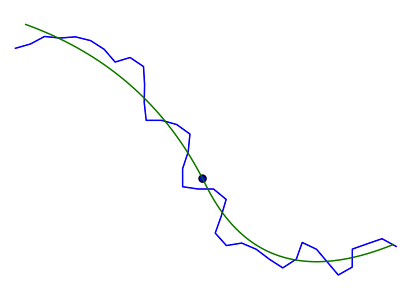
\includegraphics[scale=0.7]{plotGPAC0059.png}
  \end{center}
  \caption{Robot Posture, Gross Posture Approximation Curve (GPAC), and Local Frame Origin}
	\label{GPAC}
\end{figure}

We use the Python SciPy library's \textbf{splprep} function with a smoothness factor of $0.5$ to generate the B-spline curve.  This results in the curve shown in Figure \ref{GPAC}.  To use this curve, we define a set of parameterized functions that we use to access the curve.  First we show the function provided by the SciPy library:
\begin{equation}
O(1): \quad \beta_t(u) = ( x_u, y_u, \theta_u ),  \quad 0 \leq u \leq 1
\end{equation}

This function gives us access to the curve with a normalized parameter $u$.  The function returns the x and y coordinates of a point and the orientation of its tangent vector that correspond to the $u$ value.  The drawback to this function is that the difference of arclength between two $\beta(u)$ values is not proportional to the difference in $u$ value.  This implies that the following condition exists:
\begin{equation}
\mathbf{dist}(u_1, u_1 + K) \neq \mathbf{dist}(u_2, u_2 + K)  
\end{equation}
where the function $\mathbf{dist}()$ computes the arclength between two $u$ values on the curve, and the constant $K$ adds the same $u$ offset at two different points on the curve specified by $u_1$ and $u_2$.  What this means in practical terms is, the $u$ values cannot be relied upon to give us reproducible positions on the curve.  In particularly, if we retrieve the point $\beta_t(0.5)$, this will be close to the midpoint of the curve, but not the true midpoint and is subject to change between different curves.

We create a more accurate method that allows us to specify a point of true arclength on the curve.  We present it in the form of a parameterized function:
\begin{equation}
\label{equ:arcdist}
O(\log n): \quad \sigma_t(d) = ( x_d, y_d, \theta_d ),  \quad 0 \leq d \leq d_{max}
\end{equation}

Here $d$ is the arclength starting from the $u = 0$ terminator of the curve.  $d_{max}$ is the maximum arclength of the curve.

Though this is defined in the form of a function, it is implemented with a search algorithm.  If we pre-process the curve by uniformly pre-sampling $n$ points with $\beta_t(u)$ in $O(n)$ time, we can achieve a binary search time of $O(\log n)$ for each invocation of the function.   The $n$ parameter here corresponds to the number of samples of the curve we use to search over.  The more samples, the more accurate the function will be.   Here we use a tractable size of $n = 100$.

To perform the inverse operation for curve functions, we use the same pre-processed $n$ sample points from equation \ref{equ:arcdist} and define the following functions:
\begin{equation}
O(n): \quad \beta^{-1}_t(x, y) = u
\end{equation}
\begin{equation}
O(n): \quad \sigma^{-1}_t(x, y) = d
\end{equation}

These inverse operators find the closest sample point on the curve to $(x,y)$ and returns the sample's associated $u$ or $d$ parameter.  The correctness of these functions depend on the queried point being reasonably close to the curve, the curve not be self-intersecting, and the point not be equidistant to two disparate points on the curve.  They are $O(n)$ because we must compute the distance to all $n$ sample points.  Notice that we omit the angle portion of the curve for inverse operations.  We do not define closest point for orientations.

Since these inverse curve functions are very similar, we develop a unified algorithm that produces parallel results.  We do this to prevent duplication of search operations when similar information is needed.
\begin{equation}
O(n): \quad c_p(x,y) = (u, d, (x_p, y_p, \theta_p) )
\end{equation}

This function returns the closest point on the curve to $(x,y)$, and its associated $u$ and $d$ parameters.

Finally, we have functions that convert between $u$ and $d$.
\begin{equation}
O(\log n): \quad \mathbf{d}(u) = d
\end{equation}
\begin{equation}
O(\log n): \quad \mathbf{u}(d) = u
\end{equation}

These can be performed with a binary search on the pre-processed sample points.


\subsection{Generation of GPAC Local Frame}

%This produces a curve that approximates the general posture of the robot.  The middle point is selected by finding the location that is equidistant to the tips.  The tangent vector is used to orient the local coordinate frame.  This vector has the benefit of always pointing in the direction the robot is facing.

%and choose a point on the curve to act as our local coordinate system's origin.  This is seen in Figure \ref{GPAC}.  Notice that the direction of the curve at the origin is in the forward-backward direction making this useful as a heading reference.

For each generation of the GPAC, we can create a unique but predictable coordinate frame that represents the gross posture of the snake in the environment.  Because the GPAC only follows the general posture of the snake, regardless of its articulation, the difference in curves between generations is small and within reason.

Once we have the new GPAC, to determine the location of our new coordinate frame origin $\hat{O_t}$ with respect to $O_{19}$, we compute the following:
\begin{equation}
P_d = \sigma_t(d_{max} / 2)
\end{equation}

This specifies the halfway point along the curve in terms of arclength with respect to $O_t$.  If we had used $\beta_t(0.5)$ instead, we would have had no guarantee how close to the middle it would be and no guarantees on repeatibility.  By using the arclength function $\sigma_k()$, we have more guarantee over the location at the expense of running time.

From our new local frame $\hat{O_t}$, the orientation of the x-axis is directed in the forward direction of the snake, regardless of the articulation of the joints.  This approach now gives us the tools to make relations between snake poses where the orientations will have some correlation.  If we had insisted on using a body frame $O_{19}$ as a local coordinate frame, the orientations would have had very little correlation.  We would have had no means to relate and correct orientations between snake poses.

In the future, we will drop the $t$ subscript of a GPAC and local frame origin and only refer to them as $\beta_k(u)$, $\hat{O}_k$, and $\hat{P}_k$, where $\hat{O}_k$ is the  GPAC generated origin, $\hat{P}_k$ is the origin's location in the global frame, and $k$ is the particular pose number in the pose graph.  We describe this in more detail in Section 5.

\subsection{Geometric Transform between Poses}

\label{sec:geo_transform}

Now that we have defined a local coordinate system for the complete posture of a snake robot, we can compute a geometric transform $T_{ij}$ between two poses of the robot $\hat{P}_i$ and $\hat{P}_j$.  We take the snake poses before and after one step of the adaptive concertina gait in the GPAC local frame for each.  Each GPAC has a reference pose in the global frame, so it is only a matter of computing a transform between the two.

\section{Results}

Shown in Figure \ref{varWidth} is a plot of the snake robot¿s poses as it travels through a variable width curved pipe.  The boundaries of the pipe are drawn in green.  The black poses represent the estimated positions and the pink poses indicate the ground truth positions.  Notice that there is a discontinuity in the middle, which is likely because of the use of a reference node on an anchor with major slip.  Also, notice the sudden rotation and translation at the end caused by the slip from hitting the termination wall.   Here we do not show our collision detection and correction system, so the error introduced from the collision is shown in the plot.

Figure \ref{juncFix} showns the trajectory plot of the snake robot through a fixed-width environment with junctions.  This shows that the motion estimation has no problems estimating motion through junctions so long as the anchors are good.
 
\begin{figure}
  \begin{center}
    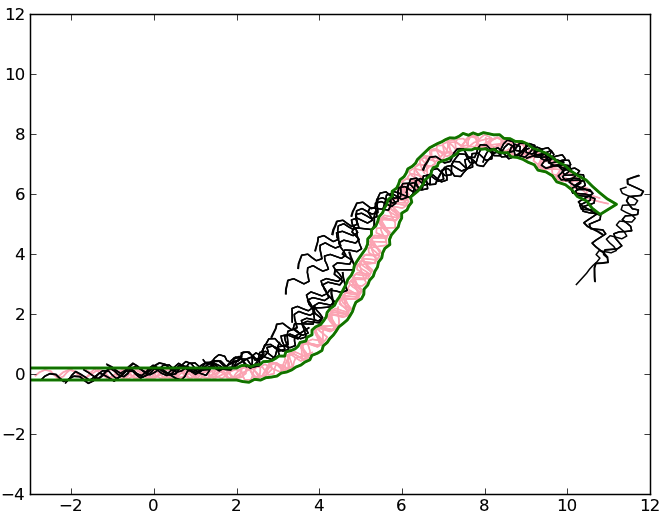
\includegraphics[width=3.4in]{plotMotionVariableWidth.png}
  \end{center}
  \caption{Estimated Trajectory of Robot through Variable-Width Pipe}
	\label{varWidth}
\end{figure}

\begin{figure}
  \begin{center}
    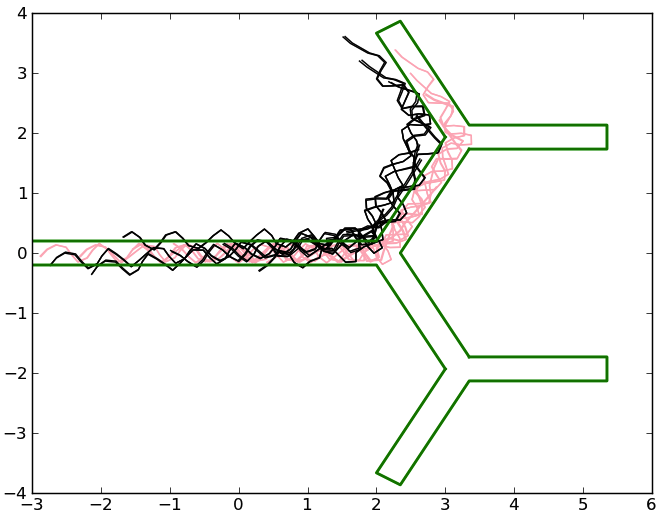
\includegraphics[width=3.4in]{plotMotionJunctions.png}
  \end{center}
  \caption{Estimated Trajectory of Robot through Fixed-Width Pipe with Junctions}
	\label{juncFix}
\end{figure}

In spite of the care taken in locomotion and motion estimation, the snake robot still accumulates positional errors.  The primary cause of this is the failure of anchors.   This can happen by the anchor originally failing to take hold, intermittent anchor motion or slip, or anchor slip caused by collision with a forward obstacle making a backward motion look like a forward motion.



The quality of motion estimation is a function of how slowly and carefully we perform our movements and maintain our anchors.  Particularly, the parameters we tune for our local stability detection and the rate of linear interpolation for movement transitions.




%\input{MSMS/msms.tex}

\chapter{Sensing with Proprioception}

\label{chap:sensing}

\section{Problem}

Now that we are able to travel through the environment and estimate our motion, the next order of business is to be able to sense the environment.  With no exteroceptive sensors, this is quite a challenging problem.  Somehow, we must use our proprioceptive joint sensors to build some information about the environment.

We use a common sense assumption that the robot's body can never intersect with an obstacle.  We call this the Obstacle-Exclusion Assumption.  If we take the corollary of this assumption, we conclude that all space that intersects with the robot's body must be free space.  If we record the robot's body posture over time, we can use this to build a map of the local environment's free space.

We need 3 key ingredients to build an accurate map of the free space in the local environment:  1) known geometry of the robot's rigid body linkages, 2) accurate joint sensors for computing kinematics, and 3) an accurate reference pose to the global frame.  If all of these things are available, we can build a local map such as shown in Figure \ref{pokeBehavior}.

\begin{figure}
  \begin{center}
    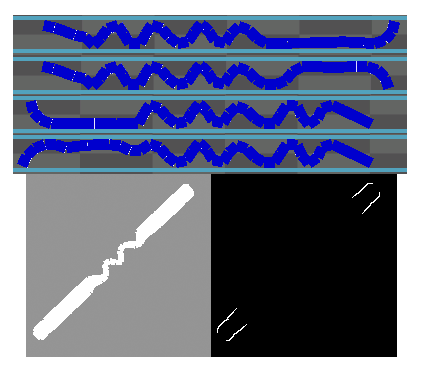
\includegraphics[scale=0.7]{PokeBehavior.png}
  \end{center}
  \caption{TODO: Remove the obstacle map.  Free space map from PokeWalls behavior.}
	\label{pokeBehavior}
\end{figure}

The map is achieved by rigidly anchoring to the environment and maintaining a set of stable reference poses.  One side of the snake's body is used to sweep the free space, making multiple snapshots of the robot's posture over time and plotting them into a map.  We discuss each aspect of our approach and show the results for a varienty of environmental configurations.

The key point here is that sensing cannot be accomplished without action.  Action by itself runs the risk of disturbing the environment or causing errors in the reference pose.  Though sensing cannot be accomplished without action, action runs the risk of modifying the result.  Special care must be taken that the risk of modifying the environment is minimized.  Here, we include the robot's body in our definition of the environment so that anchor slippage is a form of environment modification.

\section{Behavior}

In order to capture as much information about the environment as we can, we need to sweep the robot's body around as much as possible while trying to cover as much space as possible without losing our reference pose to the global frame.  Therefore, we have devised a behavior assemblage that separates responsibility for anchoring on one half of the snake and for probing the environment with the other.  This assemblage is shown in Figure \ref{pokewalls1}.  The resulting behavior is shown in Figure \ref{pokeBehavior}.

The resultant behavior sweeps the front end of the snake back and forth, impacting both sides of the pipe.  The front is gradually extended to increase the probe reach down the pipe.  Once the extension has reached the maximum, the behavior is terminated after returning the snake back to its original fully anchored Rest-State posture.

At regular intervals during the sweeping behavior at the end of each Transition termination, the posture is recorded for later processing.  The end result is an ordered list of posture vectors representing each snapshot of the robot during the behavior.  These postures are then processed into a map.

We describe each behavior in the assemblage.


\begin{figure}
\begin{center}
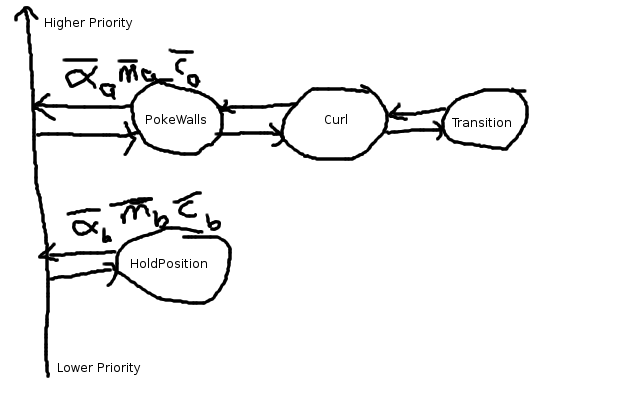
\includegraphics[scale=0.5]{4_pokewalls_1.png}
\end{center}
\caption{PokeWalls behavior assembly.}
\label{pokewalls1}
\end{figure}

%GRAPHIC
%Merge(
%PokeWalls <- Curl <- Transition
%HoldPosition
%)



\textbf{Curl:} The sweeping behavior is performed by setting a series of consecutive joints all to a 30 degree angle, resulting in a curling motion.  In a confined environment, the result of the commanded joints usually results in the snake impacting the walls of the environment.  By steadily increasing the number of joints to perform this sweeping motion, the reach of the snake is gradually increased and more space is sweeped out.

The Curl sub-behavior is responsible for commanding these joint angles given the specified joint range by the parent.  It is also responsible for executing a simple contact detection heuristic in the course of the curling behavior.  We describe both here.  

Given the top joint $j_t$ specified by the parent, the Curl behavior gives commands to the joints $(j_0 ... j_t)$, setting $\alpha_i = 0$.  All $\alpha$ are set to the following sequence of angles: $(0, 25, 30, 0, -25, -30, 0)$.  Between each movement command we use the Transition sub-behavior to manage the motion as a linear interpolation between postures.  We also wait for the tip of the snake's position to become stable for executing another movement transition.  At the end of the movement sequence and once the tip has become stable, the Curl behavior then terminates and waits to be reset by the parent. 

For the contact detection heuristic, once the joints have been set to $\alpha = 25$, the tip of the snake's position $p_a$ is computed kinematically.  The joints are then set to $\alpha = 30$ and the tip's position $p_b$ is again computed kinematically.  The Cartesian distance between $p_a$ and $p_b$ is computed.  If the value is negligible, we assume that the tip of the snake has made contact with the walls.  Otherwise, we do not assume contact has bee made.  The repeat this for the negative angle commands on the other side of the pipe.  

The way the sweeping behavior is performed is by setting the commanded position of all the joints from the tip of the snake down to a top joint simultaneously from 0 to 30 degrees.  This results in a "curling" behavior which gives the subbehavior its name.  The joints are set at angles of 0, 25, 30, 0, -25, -30, 0.


%- Curl sub-behavior
%- set all joints to -30, -25, 0, 25, 30
%- from top joint to tip
%- skip back to 0 from terminator
%- check difference between |30| and |25| to see if contact is made

\textbf{PokeWalls:} The PokeWalls behavior is responsible for specifying the range of joints that perform the Curl operation, instantiating and configuring the Curl behavior.  The PokeWalls behavior is configured with the sweeping direction on the snake, starts the Curl behavior with the joint range specified by $j_t = 6$.  It then passes through the outputs of the Curl behavior.

At the termination of the Curl behavior, PokeWalls increments $j_t$ by 2 and restarts the Curl behavior with the new parameters.  If $j_t = 10$, we then begin decrementing $j_t$ by 2 until we go back to $j_t = 6$.  Once the Curl has been executed for the second for $j_t = 6$, we terminate the PokeWalls behavior.

The PokeWalls behavior is also responsible for setting the maximum torque for each of the curling joints to be compliant.  This ensures that the posture of the snake complies to the environment and gives us as much information as possible about the structure of the free space.  If we do not have compliant joints, the curling behavior can result in disruption of the anchors and loss of our reference poses.

%is to specify which joints participate in the sweeping behavior and spawns the Curl sub-behavior.
%- receives direction
%- sets the top joint from 6 to 10 on Curl
%- walks it through Curl steps, resets and does topJoint
%- sets compliant torque from 0 to topJoint
%- sets top joint from 6 to 10 to 6 and then terminates

\textbf{Transition:}   This is the same behavior as described in Chapter 2.  It takes an initial and final posture and outputs a series of postures that provides a smooth transition between the two using interpolation.  Its parent behavior is Curl which instantiates it and resets it whenever it needs to perform a new move.

\textbf{HoldPosition:} This is the same behavior as described in Chapter 2.  It is initialized with the complete posture of the snake at the beginning of the behavior.  This posture is usually the result of the Rest-State stage of the Adaptive Step locomotion process.  It continually outputs the anchored posture.  Its output is subsumed by the output from the PokeWalls behavior in a precedence merge.  It is 2nd in the behavior ordering as shown in Figure \ref{pokewalls1}. 




\section{Proprioceptive Sensor Data}

Now that we've specified the actions we perform to sense the environment by way of the PokeWalls and Curl behavior, we now need to show how we capture sensor data and process it for consumption for our later mapping algorithms.

\subsection{Data Capture}

Once the posture of the snake has stabilized and the anchor points give us good reference poses to the global frame, our objective is take the posture vector, $\bar{\phi_t}$ at time $t$, and convert it to a 2D spatial representation of free space, $M_p$ at the current pose $p$.  We separate the tasks of spatial representation and positioning the data in the global frame.  To do this, we create a local map centered on the robot's body on which the spatial data is plotted while the robot remains in one position.

The local map is an occupancy grid representation where each cell of the grid has two states:  \emph{unknown} or \emph{free}.  If the body of the robot is present on a cell, this cell is marked \emph{free}.  Otherwise, it is \emph{unknown}.  It is unknown instead of \emph{occupied} because our approach does not have any means to specifically observe obstacles beyond contact detection heuristics.  The heuristics are not accurate enough to plot their positions into the occupancy grid, so we leave the cells unknown for now.

The size of a cell is chosen for the desired accuracy we require.  Smaller cell sizes require more computational time, but larger cell sizes will result in blocky maps.  We choose our cell dimensions $s_p \times s_p$ to be
%pixelSize
$s_p = \frac{l}{3} = 0.05$, or one third the length of a snake segment.

Given that we now have our cell dimensions, we can compute the dimensions of our local map to be 
%mapSize
%$s_M = l * N+ 2 + 2$,
$s_M = l * N$ + 4,
where $l$ is the segment length and $N$ is the number of segments.  $s_M$ is the maximum length from the origin at the center of our local coordinate system.  We want the dimensions to be larger than the worse case scenario of the snake's posture.  We also include an extra padding of $4$ to ensure that the snake never reaches the boundary of the grid.

The number of cells or pixels in our local map will be $n_p \times n_p$ where
%numPixel
$n_p = \bigg\lceil \frac{2 s_M}{s_p} + 1 \bigg\rceil$.  This equation ensures that $n_p$ is an odd integer.  The $+1$ factor adds an extra cell whose center will act as the origin of our local coordinate system.


Now that we have the dimensions of the grid space and its relation to Cartesian space, we need to know how to convert points from one space to the other.  To convert a grid index $(i_x,i_y)$ to Cartesian space point $(p_x,p_y)$ centered within the cell, we compute the following:
%$p_x = (i_x - n_p/2 - 1)*(s_p/2) + s_p/2$
%p_y = (i_y - n_p/2 - 1)*(s_p/2) + s_p/2$
\begin{eqnarray}
\label{eqn:g_to_p}
%p_x = \bigg(i_x - \frac{n_p}{2} - 1\bigg)\frac{s_p}{2} + \frac{s_p}{2} \\
%p_y = \bigg(i_y - \frac{n_p}{2} - 1\bigg)\frac{s_p}{2} + \frac{s_p}{2} 
p_x = \bigg(i_x - \bigg\lfloor\frac{n_p}{2}\bigg\rfloor \bigg)\frac{s_p}{2} \\
p_y = \bigg(i_y - \bigg\lfloor\frac{n_p}{2}\bigg\rfloor \bigg)\frac{s_p}{2}
\end{eqnarray}


Conversely, to find the index of a cell $(i_x,i_y)$ that contains a Cartesian point $(p_x,p_y)$, we compute the following:
%divPix
%$divPix = \lfloor \frac{\frac{2 s_M}{s_p}}{s_M} \rfloor$
%$i_x = \lfloor point[0]*2/s_p \rfloor + n_p/2 + 1$
%$i_y = \lfloor point[1]*2/s_p \rfloor + n_p/2 + 1$
\begin{eqnarray}
i_x = \bigg\lfloor \frac{p_x}{s_p} \bigg\rceil + \bigg\lceil\frac{n_p}{2}\bigg\rceil \\
i_y = \bigg\lfloor \frac{p_y}{s_p} \bigg\rceil + \bigg\lceil\frac{n_p}{2}\bigg\rceil
\end{eqnarray}


Now that we have the tools for mapping positions in physical space to our grid space occupancy map, we need data to plot into the map.  Using kinematics, we compute the geometry of the posture of the snake.  We can represent this by a 4-sided rectangle for each segment of the snake.  We set the origin of our coordinate system on segment 19 and joint 19 which is the midway point for $N = 40$.  We define this to be:
\begin{equation}
O_t = (x_{19}, y_{19}, \theta_{19}) = (0, 0, 0)
\end{equation}
where $O_t$ is the pose of $P_{19}$ in the local frame at time $t$.  This may change which is explained in section \ref{sec:ref_stable}.

To compute the segment 19 rectangle, starting from the origin for $k = 19$, $x_k = 0$, $y_k = 0$, and $\theta_k = 0$, we compute the following:

%From 19, towards N
\begin{equation}
\label{equ:rect1}
\begin{array}{l}
\displaystyle x_{k+1} = x_k + l \cos(\theta_k) \\
\displaystyle y_{k+1} = y_k + l \sin(\theta_k) \\
\displaystyle \theta_{k+1} = \theta_k - \phi_{k+1} \\
\displaystyle p_1 = \bigg( x_{k+1} - \frac{w\sin(\theta_k)}{2} , y_{k+1} + \frac{w\cos(\theta_k)}{2}\bigg) \\
\displaystyle p_2 = \bigg( x_{k+1} + \frac{w\sin(\theta_k)}{2}, y_{k+1} - \frac{w\cos(\theta_k)}{2} \bigg) \\
\displaystyle p_3 = \bigg( x_{k+1} - l\cos(\theta_k) + \frac{w\sin(\theta_k)}{2}, y_{k+1} - l\sin(\theta_k) - \frac{w\cos(\theta_k)}{2} \bigg) \\
\displaystyle p_4 = \bigg( x_{k+1} - l\cos(\theta_k) - \frac{w\sin(\theta_k)}{2}, y_{k+1} - l\sin(\theta_k) + \frac{w\cos(\theta_k)}{2} \bigg) \\
\displaystyle R_k = (p_4,p_3,p_2,p_1)
\end{array}
\end{equation}

The result is the rectangle polygon $R_k$, which represents the rectangle of the segment $19$.  The next reference pose $(x_{k+1},y_{k+1},\theta_{k+1})$ is also computed.  Here $k+1=20$.  To compute the k\textsuperscript{th} rectangle for $k \geq 19$, we need only compute this iteratively until we reach the desired segment.

To perform this backwards, to find segment $18$, where $k+1=19$ and $(x_{k+1}, y_{k+1}, \theta_{k+1}) = O_t$, we compute the following:

\begin{equation}
\label{equ:rect2}
\begin{array}{l}
\displaystyle \theta_k = \theta_{k+1} + \phi_k \\
\displaystyle x_k = x_{k+1} - l \cos(\theta_k) \\ 
\displaystyle y_k = y_{k+1} - l \sin(\theta_k) \\
\displaystyle p_1 = \bigg( x_{k+1} - \frac{w\sin(\theta_k)}{2} , y_{k+1} + \frac{w\cos(\theta_k)}{2}\bigg) \\
\displaystyle p_2 = \bigg( x_{k+1} + \frac{w\sin(\theta_k)}{2}, y_{k+1} - \frac{w\cos(\theta_k)}{2} \bigg) \\
\displaystyle p_3 = \bigg( x_{k+1} - l\cos(\theta_k) + \frac{w\sin(\theta_k)}{2}, y_{k+1} - l\sin(\theta_k) - \frac{w\cos(\theta_k)}{2} \bigg) \\
\displaystyle p_4 = \bigg( x_{k+1} - l\cos(\theta_k) - \frac{w\sin(\theta_k)}{2}, y_{k+1} - l\sin(\theta_k) + \frac{w\cos(\theta_k)}{2} \bigg) \\ 
\displaystyle R_k = (p_4,p_3,p_2,p_1)
\end{array}
\end{equation}

The result is the same polygon as well as the new reference pose for segment $18$.  To compute the k\textsuperscript{th} segment rectangle for $k < 19$, we need only use this equation iteratively.  Computation of all $N$ rectangles results in the set of rectangles $\bar{R_t}$ for the current posture.

Now that we have a set of rectangles which represent the geometry of the robot in its current posture, we want to plot its occupied space into the local occupancy map.  To do this, we need to convert polygons in Cartesian space into sets of grid points.  To do this, we use a point-in-polygon test algorithm for each of the pixels in the map.

The simplest approach is as follows.  For each pixel, convert it to Cartesian space, test if it's contained in any of the polygons, and if it is, set the pixel to \emph{free}.  Otherwise, let the pixel remain in its current state.  The pseudocode for the point-in-polygon test for convex polygons derived from \cite{orourke98} is seen in Algorithm \ref{alg:pip_test}.

\begin{algorithm}
\caption{Point-in-Polygon Test}          % give the algorithm a caption
\label{alg:pip_test}
\begin{algorithmic}

\State $R \Leftarrow $ rectangle
\State $P \Leftarrow $ point

\For{$i = 0 \to 4$}
\State $A_x \Leftarrow R[i \bmod 4][0] $
\State $A_y \Leftarrow R[i \bmod 4][1] $
\State $B_x \Leftarrow R[(i+1) \bmod 4][0] $
\State $B_y \Leftarrow R[(i+1) \bmod 4][1] $
\State $C_x \Leftarrow P[0] $
\State $C_y \Leftarrow P[1] $

\If{$!((Bx - Ax) * (Cy - Ay) - (Cx - Ax)*(By - Ay) \geq 0)$}
\State return False
\EndIf
\EndFor
\State return True

\end{algorithmic}
\end{algorithm}

\begin{figure}
  \begin{center}
    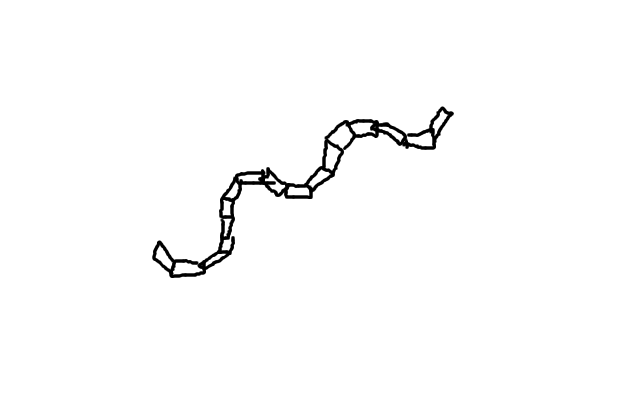
\includegraphics[scale=0.7]{4_snapshot_1.png}
  \end{center}
  \caption{Snapshot of $\bar{\phi_t}$ in local coordinates.}
	\label{snapshot}
\end{figure}


A single snapshot of the snake posture plotted into the local map is shown in Figure \ref{snapshot}.  The posture $\bar{\phi_t}$ is captured, the rectangles $\bar{R_t}$ representing the body segments are computed from kinematics, each pixel $(i_x,i_y)$ of the map $M_p$ is converted to Cartesian space point $(p_x,p_y)$ and checked by the point-in-polygon algorithm if it is in a rectangle $R_k$.  If it is, $M_p(i_x,i_y)$'s value is set to \emph{free}.  This is repeated for each point in each rectangle for a posture snapshot at time $t$.

\begin{figure}
  \begin{center}
    
\includegraphics[scale=1.0]{localOccMapSingle0.png}
  \end{center}
  \caption{Single forward sweep. }
	\label{single_sweep}
\end{figure}

\begin{figure}
  \begin{center}
    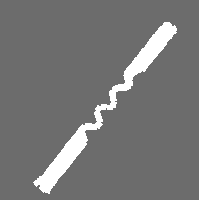
\includegraphics[scale=1.0]{localOccDouble.png}
  \end{center}
  \caption{Forward and backward sweep.}
	\label{double_sweep}
\end{figure}



While running the PokeWalls behavior, we periodically take snapshots at the conclusion of each Transition step and plot them into the map.  A complete sweep with the PokeWalls behavior is shown in Figure \ref{single_sweep}.   Furthermore, if we also perform a sweep with the other side of the snake, we can get a map like Figure \ref{double_sweep}.

Notice in Figure \ref{double_sweep} that there is a gap in the free space data in the center of the body.  These segments at the center remain immobilized throughout the sweeping process and never give extra information.  This gap in the center is our "blind spot" for this configuration.  It is necessary that the center remain immobilized to ensure anchors do not slip so that we maintain correct reference poses to the global frame.

We have no guarantee that there are obstacles at the boundaries of our free space map.  We also have no quick way to determine if the boundary of our map is an obstacle or a frontier.  While the boundaries at the front and back are usually assumed to lead to more free space, anywhere along the sides could be a missed side passage that the snake failed to discover due to it being too small or being in our blind spot.  To combat this situation, we either must perform laborious and time-consuming contact probing of every surface, or use quick-and-dirty contact detection heuristics to guide our mapping process.

\subsection{Data Processing}

Once we have the raw sensor data successfully plotted into a local occupancy map, we must convert this data into a form that is useful for our mapping algorithms.  Here, we present three different forms of data processing that we use in our approach.

\subsubsection{Convex Hull}

One way we process our free space data is by taking its convex hull.  In theory, this would create some smooth boundaries and can plausibly represent the true local space under some certain conditions.   The definition of the convex hull is, given a set of points $P$, find the convex polygon $H$ with minimum area that contains all of $P$.

To create our set of points $P$, for each pixel $(i_x,i_y)$ of the occupancy map $M_p$ whose state is \emph{free}, convert the pixel to Cartesian space point $(p_x,p_y)$ using Equation \ref{eqn:g_to_p} and add to $P$.  Using any convex hull algorithm, produce the resultant polygon in Cartesian space.   For our work, we use the convex hull algorithm available in CGAL \cite{cgal:hs-chep2-12b}.

\begin{figure}
  \begin{center}
    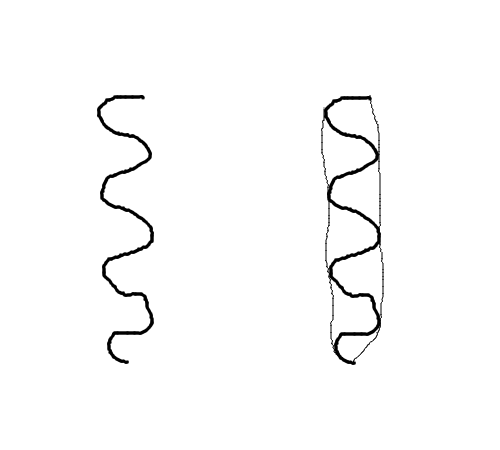
\includegraphics[scale=0.9]{4_convex_freespace1.png}
  \end{center}
  \caption{Free space data before and after convex hull.}
	\label{convex_free1}
\end{figure}

\begin{figure}
  \begin{center}
    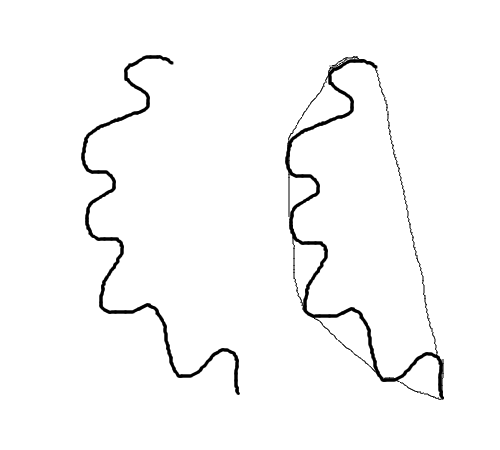
\includegraphics[scale=0.9]{4_convex_freespace2.png}
  \end{center}
  \caption{Free space data of curved posture before and after convex hull.}
	\label{convex_free2}
\end{figure}

An example of the convex hull operation on our free space data set appears in Figure \ref{convex_free1}.  We can see for the case that the snake is in a straight pipe, the convex hull creates a natural representation of the local pipe environment, filling in the blanks of our blind spot.  However, if the pipe is curved as in Figure \ref{convex_free2}, the convex property of the polygon necessarily erases any concave properties of the environment.  This also removes any sharp features of the environment such as corners.  Therefore, any use we may have for the convex hull will be in limited situations.


%A common algorithm from computational geometry that finds a minimum convex polygon that fits all the points.  The points in our case are the grids that are marked with free space.   Convert theses pixesl to points at their centers, and we have input for a convex polygon.  The results look like Figure 0.  Cite \cite{cgal:hs-chep2-12b}

%This has the capability of smoothing over the gaps from the blind spots.  Has shortcomings.  Loses corners.

%Has some uses, but for curved pipes, we lose critical information about the true pipe dimensions and their curved topology.  Does not represent nonconvex features.

\subsubsection{Alpha Shape}

An alternative to the convex hull is the alpha shape \cite{Edelsbrunner:1983p772}.  Like the convex hull, it creates a polygon or polygons that contain all the points.  Unlike the convex hull, it can construct a containing polygon with concave or even hole features.  

\begin{figure}
  \begin{center}
    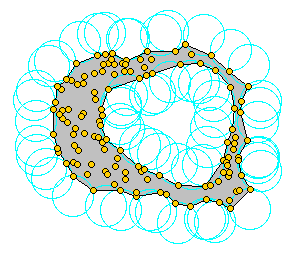
\includegraphics[scale=0.7]{alphashape.png}
  \end{center}
  \caption{Alpha Shape example from \cite{cgal:d-as2-12b}}
	\label{alpha_cgal}
\end{figure}

To construct the alpha shape, first we choose a radius $r$ for a circle $C$.  Next, if a pair of points $p_i$ and $p_j$ can be put on the boundary of $C$ where no other point is on or contained by $C$, we add an edge between $p_i$ and $p_j$.  The result is seen in Figure \ref{alpha_cgal}

\begin{figure}
  \begin{center}
    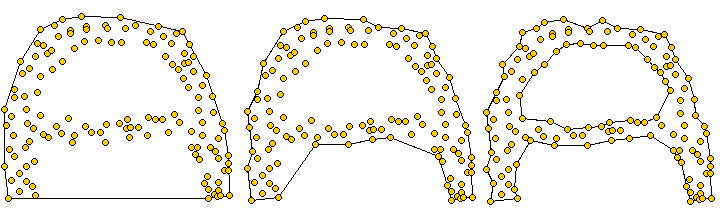
\includegraphics[scale=0.6]{4_alpha_radius.png}
    %\includegraphics[scale=0.7]{alpha_example2.gif}
  \end{center}
  \caption{Alpha Shape changing radius from \cite{cgal:d-as2-12b}}
	\label{alpha_cgal2}
\end{figure}

By changing the radius size, we can tune how much smoothing we want to occur in the resultant polygon, seen in Figure \ref{alpha_cgal2}.  If we set the radius to $r = \infty$, the alpha shape reduces to the convex hull.  Therefore, this is a kind of "generalized convex hull" algorithm.

\begin{figure}
  \begin{center}
    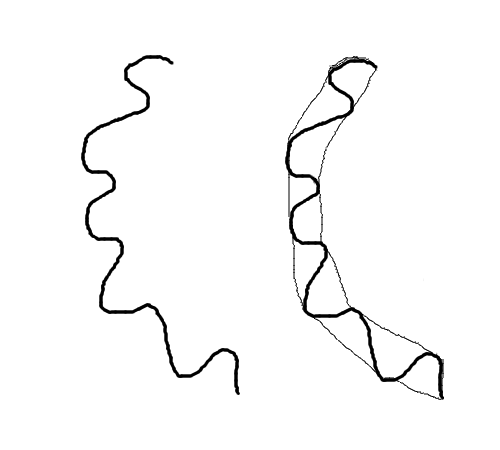
\includegraphics[scale=0.9]{4_alpha_freespace2.png}
  \end{center}
  \caption{Alpha hull of free space data.}
	\label{alpha_free2}
\end{figure}

The benefit to this approach is that we can now capture the concave features of some of our local maps where the convex hull failed.  Where Figure \ref{convex_free2} shows the convex hull, Figure \ref{alpha_free2} shows its corresponding alpha shape.  In both cases, the blind spot it smoothed over and filled in.  This approach still suffers from the loss of sharp salient corner features, but the gross topology of the local environment has been captured.

For clarity, we refer to the alpha shape of our local free space as the \emph{alpha hull} from here on out.


\subsubsection{Medial Axis}

Although polygons that represent the sweeped free space are useful, we need something that is more compact that also filters out the smoothing effects of blind spots and sharp features.  That is, we want an approach where the negative effects of missing data, erroneous data, and loss of salient features are minimized.

For this purpose, we compute the medial axis, also sometimes known as thinning or skeletonization [cite].  This concept takes a shape and reduces it to a path or series of edges that follow the "spine" of a shape.  Approaches range from a strict computational geometry approach such as the Voronoi diagram to image processing approaches of image thinning and skeletonization that erode a pixelized shape until the skeleton is all that remains [cite].

%Skeletonization of a binary image.
%Black values (0) mean object and white values (1 = 255) background.
%Source: Parker, J.R. Algorithms for image processing and computer vision.
%				New York, NY: John Wiley & Sons, 1997. 417p. pp. 203-218.
%
%Program adapted to C/OpenCV by Jose Iguelmar Miranda.
%March, 2010.
%I have also a Java version of this program.

\begin{figure}
  \begin{center}
    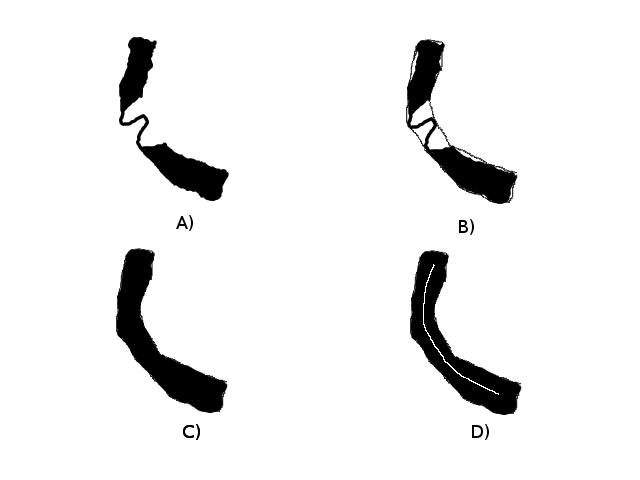
\includegraphics[scale=0.9]{4_medial_process.png}
  \end{center}
  \caption{Process of generating medial axis.}
	\label{medial1}
\end{figure}

\begin{figure}
  \begin{center}
    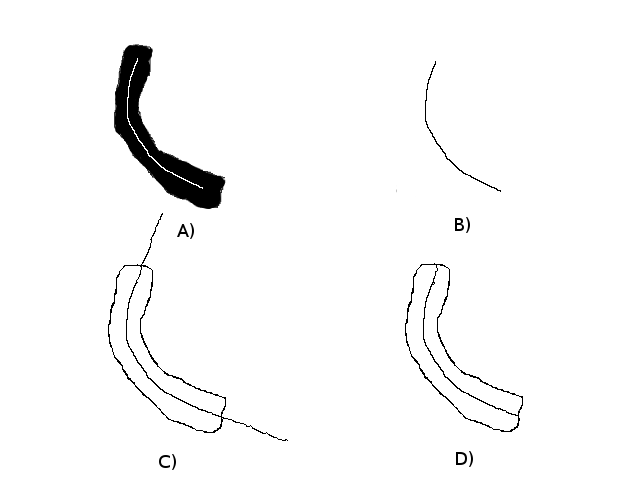
\includegraphics[scale=0.9]{4_medial_process2.png}
  \end{center}
  \caption{Process of generating medial axis.}
	\label{medial2}
\end{figure}

We are interested in extracting the medial axis of the alpha hull generated from our free space map.  Since the alpha hull smooths the boundaries of the free space map, generating a medial axis will give us a topological representation of the free space that is resistant to boundary features.  Given the free space map in Figure \ref{medial1}a, and its corresponding alpha hull in Figure \ref{medial1}b, the alpha hull's conversion back to an image in Figure \ref{medial1}c, and its resultant medial axis shown in Figure \ref{medial1}d.  We use the skeletonization algorithm from [ParkerJR] \footnote{C/OpenCV code written by Jose Iguelmar Miranda, 2010}.

We can see that the medial axis roughly corresponds to the topological representation of the pipe environment.  However, it is crooked, pixelated, and does not extend the full length of the data set.  We further treat this data to give a more useful representatation.

Starting with the result from Figure \ref{medial1}d shown in Figure \ref{medial2}a, we create a minimum spanning tree (MST) graph where each node is a pixel from the medial axis and an edge is added between two nodes if their corresponding pixels are neighbors, shown in Figure \ref{medial2}b.

This MST has many leafs due to the artifacts of pixelation.  We can simply prune the whole tree by sorting all nodes by degree, and removing the nodes with 1 degree and their corresponding edges.  In most cases, this will leave us with a single ordered path of nodes with no branches.  In some cases, we will have a branch if the original free space map shows evidence of a junction.

In the case of a single path, our next step is to extend this path to full extent of the original shape.  We begin by fitting a B-Spline curve to the ordered path.  With an appropriate smoothing parameter, the spline curve will follow the path of the ordered points but will ignore the jagged edges from pixelation.  We then uniformly sample points along this curve to convert it back to an ordered set of points.  We extend this path in the front and back by extrapolating more points along the direction specified by the curve tip, as in Figure \ref{medial2}c.  Multiple tangent vectors are sampled along the tip neighborhood and their direction is averaged to get a direction that is immune to spline curving artifacts at the terminals.  Finally, the series of points is cut off once the extrapolated points cross the alpha hull boundary, shown in Figure \ref{medial2}d.

In the case that we have a branch, we perform this series of operations for the path between each combination of pairs of terminals.  For each medial axis of a free space map, there are $n = 2 + B$ end points where $B$ is the number of branches.  The number of unique paths of a medial axis is found by ${n \choose 2}$ since we are using the MST and there is a unique path between each pair of points.

The final form is a compact representation of the topology of the local free space that removes the noise and uncertainty of the boundary and allows us to only represent the area we can move through.  This has a number of uses for our map-making that we describe in the next chapter.  

% environment -> free space map -> alpha hull -> image of alpha hull interior -> medial axis -> graph -> MST -> Spline -> sampled points -> extrapolation -> cutoff at boundary -> overlap of environment 

\section{Failures}

Since the possibility of error occuring in our free space maps is very real and has the consequences of making the data near-useless, we want to do all we can to prevent and mitigate any failure conditions.  As the primary source of error is anchor slip, we do all we can to focus on this issue while probing the environment.  We use a number of techniques for both prevention and detection of error.  We describe all of our approaches below.

\subsection{Error Prevention}

We have 6 strategies for preventing anchor slip during the course of probing the environment.  These are the following:

\begin{enumerate} \itemsep 1pt \parskip 0pt \parsep 0pt
  \item Prescriptive Stability
  \item Local Stability
  \item Smooth Motion
  \item Averaging Reference Poses
  \item Separation of Sweep Maps
\end{enumerate}

The first three we have discussed earlier, with prescriptive stability and local stability in section \ref{sec:anchors} and smooth motion in section \ref{sec:smooth}.  We use prescriptive and local stability to determine which reference poses are available to be activated.  Whereas, smooth motion through the use of linearly interpolated steps by using the Transition behavior reduces the chance that our anchors will slip. 

The prescriptive stability selection of the PokeWalls behavior requires the robot to only use the anchored portion of the snake body for reference poses.  In particular, it is very conservative, where only the segments at the very back and mechanically isolated from any of the sweeping motions in the front will be used for reference.  This reduces the chance that any perturbations from the probing motions will have an effect on any of the active reference poses that we are using.

\subsubsection{Averaging Reference Poses}

For our fourth strategy, when actually using the reference poses to compute the position of the snake in our local free space map, we want to use as many of the reference poses as possible while filtering out any errors that would occur from possible pathological cases.   If just one reference pose is erroneous and we use that reference pose to compute position of the snake in free space,  it will severely damage our results.  We want to mitigate the possibility of negative effects by taking the average of a set of reference poses when computing a snake's position.

For instance, if we wanted to compute the origin of our local free space map in global space, we would compute the kinematic position of joint 19 with respect to some active reference pose $P_k$ on joint and segment $k$.  Using equation \ref{kinem1} or \ref{kinem2}, we compute the position of $P^{k}_{19}$.  For every $P_k$ we use, we compute a new $P^{k}_{19}$ that is possibly different.  We then take the average of all of the computed $P^{k}_{19}$ poses and take that as our best guess for $P_{19}$. 

\begin{figure}
  \begin{center}
    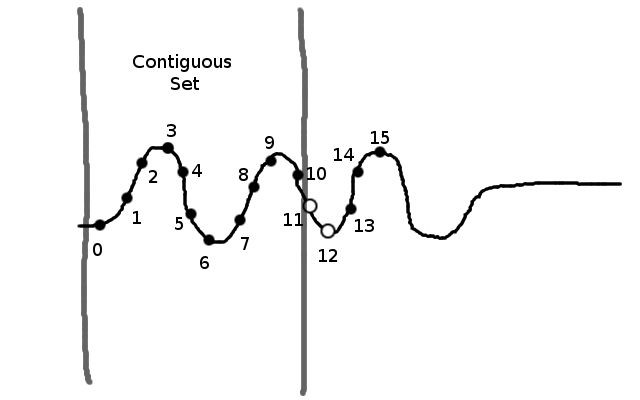
\includegraphics[scale=0.6]{4_ref_averaging.png}
  \end{center}
  \caption{Largest set of contiguous reference poses.}
	\label{ref_average}
\end{figure}

How do we select the set of active reference poses from which to compute our estimated snake pose?  Of all available active reference poses, our approach is to use the largest set of contiguous poses to compute the average target pose $P_{19}$.   Our assumption is that if we have a series of reference poses from 0 to 15, and 11 and 12 are deactivated, it is highly possible that 13, 14, and 15 are invalid because whatever caused 11 and 12 to be activated will likely have an effect on its neighbors.  The larger section from 0 to 9 has less likelihood of being corrupted since more of our sensors indicate stability.  Furthermore, if one or two of these reference poses are corrupted, having a larger set reduces the weight of an erroneous value.  This example is shown in Figure \ref{ref_average}.

\subsubsection{Separation of Sweep Maps}

Our fifth and final strategy for preventing errors in our sensor maps is to divide the forward sweep phase and backward sweep phase into separate maps.  From our experiments, we determined that a consistent source of error occurs when switching the anchoring responsibility from the back half of the snake to the front half.  The series of events of retracting the front half of the snake to anchors and extending the back half for sweeping tends to cause some discontinuity between the consensus of the back reference poses and the front reference poses.  This will show with a very distinct break in the combined free space map.

\begin{figure}
  \begin{center}
    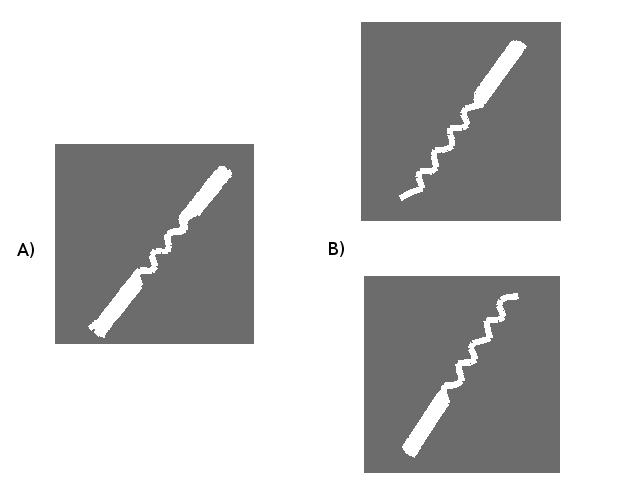
\includegraphics[scale=0.6]{4_sweepmap_1.png}
  \end{center}
  \caption{Separation of Sweep Maps.}
	\label{ref_sweep_sep}
\end{figure}

To avoid this problem, we instead create two free space maps: one for the front sweep and one for the back sweep.  What was previously shown in Figure \ref{ref_sweep_sep}a will now become the pair of maps shown in Figure b.  Not only does this avoid corrupting the free space data in the map, but it allows us to treat the relationship between the two maps as a separate problem for which there are multiple solutions.  Our previous sensor processing algorithms work just as well because the alpha shape of the half-sweep free space map will result in an alpha hull from which an equivalent medial axis can be extracted.  

We discuss our approach to managing the relationship between the two half-sweep local maps in the next chapter.

%The fourth strategy is in regard to how to use the reference poses to compute the pose of a robot segment in space.  Instead of selecting one reference pose to use and hoping that it is 100 percent correct, we take a set of reference poses and average the computed position of a target segment.  How we select the set of references to use is by looking for the largest contiguous set.  That is, reference poses that are active and are all neighbors, we select the largest set.  If for instance, a set of 15 reference poses are used in time $t$ and later reference pose 10 becomes deactived, for time $t+1$, we assume that the poses $0-9$ are still immobile and not $11-15$.  Our heuristic assumes that it is much easier to move less segments than more.  

%-- averaged position from the back anchor reference poses

%-- only use backy-back reference poses to minimize possibility of bad reference poses being used.   Prescriptive stability is very conservative.

% Separation of forward sweep and backward sweep local maps.  Do not merge them but keep them separate and correctable.
% Error comes from the switch in posture from back-anchor/forward sweep to front-anchor/backward sweep


\subsection{Error Mitigation}

In the case that error is introduced into our local free space map, we are interested in mitigating its negative effects.   We have developed two approaches for handling error when it occurs during sensing.

Since we start our mapping process by determining the global pose of the local origin $P_{19}$, error occurs when $P_{19}$ is no longer in its proper place.  Either it moves by translation or more commonly and critically, it experiences rotational error.  

\subsubsection{Reference Stabilization}
\label{sec:ref_stable}

\begin{figure}
  \begin{center}
    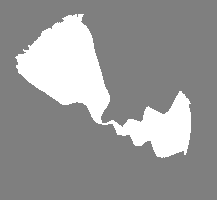
\includegraphics[scale=1.0]{localMapError.png}
  \end{center}
  \caption{Local map rotational error.}
	\label{ref_rot_error}
\end{figure}

A sudden rotation of $P_{19}$ may occur, caused by any of the reasons detailed in Section \ref{sec:anchors}.  The consequences of rotational error is that the entire body of the snake will rotate around the origin within the local map.  This will result in a map feature shown in Figure \ref{ref_rot_error}.

We proactively combat this possibility by running a reference stabilization algorithm that continually corrects the local origin $O_t$ for $P_{19}$ in the local map at time $t$.  For $t=0$, the origin is $(0,0,0)$ for inputing into the equations \ref{equ:rect1} and \ref{equ:rect2}.  However, for each time step, we wish to calculate an $O_t$ that is the most "stable" in case $P_{19}$ becomes destabilized.

To do this, we remark that during the probing phase, the back anchored section of the snake as a whole will remainly roughly in the same tight space even if its joints and ssegments should wobble and slip.  Short a large amount of translational slipping down the pipe, taken as a whole, the body should remain in the same place.  Therefore, in the local free space map, the back anchored portion should of the snapshot time $t$ should also remain in the same neighborhood of the back anchor snapshot at time $t-1$.  

\begin{figure}
  \begin{center}
    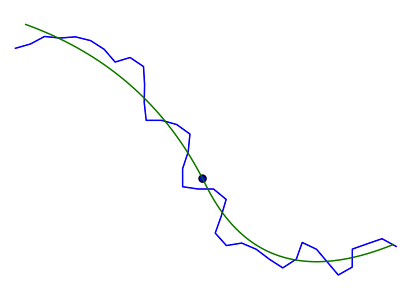
\includegraphics[scale=1.0]{plotGPAC0059.png}
  \end{center}
  \caption{Gross Posture Approximation Curve of sample posture.}
	\label{ref_gpac}
\end{figure}

We enforce this observation by fitting B-spline curve $\beta_t$ and $\beta_{t+1}$ along the points that make up the reference poses of the back anchor segments for both the current and previous snapshots.  The B-spline curves are calibrated to smooth out the sinusoidal anchoring posture of the snake body and instead reflect the gross posture of the body in the confined environment as shown in Figure \ref{ref_gpac}.   We then find a $(\delta x, \delta y, \delta \theta)$ for $\beta_{t+1}$ such that the two curves are aligned and then we update $O_{t+1}$ to reflect this.

This approach prevents sudden rotational errors from occurring and corrects the snake's estimated pose in the local map while we are capturing sensor data by generating a new $O_{t+1}$ that is consistent with past data.  So even if the snake's body is wobbling or slipping, we will likely produce consistent sensor data.
 

%Our goal is to detect when this first occurs and compensate to keep the map consistent.  We accomplish this by determining if the new posture snapshot suddenly jumps out of the local free space area we have already mapped.  The time between snapshots is very short and the snake probe is moving slowly enough that this is a reasonable assumption.

%We accomplish this by doing the following.   At every timestep $t$, we have previously computed the alpha hull $H_{t-1}$ for the current free space map.   For the current posture $\bar{\phi_t}$, and for its position in the free space map using equations \ref{equ:rect1} and \ref{equ:rect2} and starting from the origin $O_{t-1}$, determine if its position breaches the boundary of $H_{t-1}$ by distance $d_h$.

%--- we suppose that a significant rotational error has occurred.  In this case, we alter the location of the root pose from origin to an offset that keeps the posture inside the polygon boundary.  
%--- Correction is achieved by creating a spline of the back segments of the original and the current back posture.  The back splines are re-aligned and the pose of the root node is recomputed using this is a constraint.

\subsubsection{Minimum Data Reduction}

If all of our error prevention and reference stabilization strategies fail and we still produce corrupted data, we wish to detect this fact and handle it accordingly.  As we said, most error creates a rotation effect around the origin $O_t$, and produces an effect shown in Figure \ref{ref_rot_error}.  We call this sensor artifact a \emph{bowtie}.

\begin{figure}
  \begin{center}
    \includegraphics[scale=0.6]{4_bowtie_detect.png}
  \end{center}
  \caption{Width distribution for detecting a bowtie.}
	\label{bowtie}
\end{figure}

We develop a bowtie detector where we expect high widths on the exteriors and a tight width in the center shown in Figure \ref{bowtie}.  If we detect these conditions, then we declare this a bowtie and the proceed to the next step.  Note that this approach assumes that we will not encounter an environmental feature that approximates a bowtie.  We will address environments with bowtie features in future work.

\begin{figure}
  \begin{center}
    \includegraphics[scale=0.5]{4_snapshot_1.png}
  \end{center}
  \caption{FIXME: Minimum data of anchored position if bowtied: only initial posture.}
	\label{snapshot2}
\end{figure}

Once we've declared the sensor data to be bowtied, we then reduce the sensor data to minimal amount of correct information.  This would be the initial posture of the snake before it started its sweep as shown in Figure \ref{snapshot2}.  We can still treat this data with sensor processing and generate an alpha hull and a medial axis that is correct.  However, we lose data that would indicate any branches or salient wall features.  In our approach, we prefer missed data instead of bad data, so this is acceptable.

\section{Results}



\chapter{Building a Map with a Pose Graph}

\section{Problem}

Now that we have established our methodology for sensing the free space of the environment, we need some way of integrating our local free space maps into a map representation.  At each anchored position between locomotion steps, we create two free space maps for the front and back probe sweeps respectively.  Each local map is plotted in a local coordinate frame centered on the middle of the robot.  These local maps created while the robot is traveling through the environment need to be stitched together to make a global map.

We develop an approach to build a map using a \emph{pose graph} representation [cite].  We explain our specific implementation in the next section and demonstrate the results of our approach.

\section{Pose Graph Representation}

Our approach is derived from Pose/Feature Graphs [Olson2008] but differs in that we do not have feature nodes.  Since we only have pose nodes, we call it a Pose Graph.  This is similar to other graph-based approaches such as Constraint Networks, Graph-Based SLAM or Network-Based SLAM.

\begin{figure}
  \begin{center}
    \includegraphics[scale=0.7]{5_pose_graph_basic.png}
  \end{center}
  \caption{Simple Pose Graph}
  \label{fig:simple_pose_graph}
\end{figure}

A pose graph is defined by a set of nodes $V$ and a set of edges $E$.  Each node $v_k \in V$ represents a position of the robot in the environment and its collected sensor data.  Each edge $e_{ij} \in E$ represents a geometric relation between the nodes $v_i$ and $v_j$.  A simple example is shown in Figure \ref{fig:simple_pose_graph}.

Each \textbf{node} $v_k \in V$ is associated with a corresponding pose $\hat{P_k}$ and local free space map $M_k$ created at that pose.  The pose is the location of the GPAC origin of the snake robot originally defined in Section \ref{sec:GPAC}.  The local map $M_k$ is the free space data originally defined in Chapter \ref{chap:sensing}.

Each \textbf{edge} $e_{ij} \in E$ is associated with a geometric transform $T_{ij}$ and a covariance matrix $C_{ij}$ between the nodes $v_i$ and $v_j$.  $T_{ij}$ represents the geometric transform between $\hat{P}_i$ and $\hat{P}_j$ and is derived from the motion estimation system as detailed in Section \ref{sec:geo_transform}.  Other derivations for the geometric transform are possible and are described in the next section.  The covariance $C_{ij}$ is represents the uncertainty of $T_{ij}$ between the two poses.  Together the $T_{ij}$ and $C_{ij}$ form a \emph{constraint}.
%The reason for the use of GPAC for our poses now becomes apparent as two consecutive poses will have similiar pose angles.

We add nodes and edges to the pose graph as the robot travels through the environment and collects sensor information.  We can later use a batch optimization algorithm to find the minimum error satisfaction of the constraints to produce a corrected map.  The correctness of the resultant map depends on the quality of the constraints.  That is, the correctness of the geometric transform $T_{ij}$ and an accurate representation of its uncertainty $C_{ij}$.

%As the pose graph is built, we can input the graph representation into a batch optimization algorithm that adjustes the poses of $V$ to produce a minimum error satisfaction of the constraints represented by the geometric transforms and uncertainties of $E$.  Since our current approach is in 2D, we use the freely available 2D network optimizer TORO [cite].  This will perform map correction so long as the constraints in the pose graph are chosen wisely.

At the end of each AdaptiveStep locomotion step, we create two new nodes for the robot snake's anchored position.  The two nodes represent the snake's forward sweeping behavior and backward sweeping behavior respectively.  Each node contains the local map created from the execution of a PokeWalls behavior shown in Figure \ref{ref_sweep_sep}.  If $k=n_v$ is the total number of nodes in the pose graph, the newly created nodes are $v^f_{k}$ and $v^b_{k+1}$ for the forward and backward sweeps respectively.  Our graph starts to look like in Figure \ref{fig:paired_pose_graph}.

\begin{figure}
  \begin{center}
    \includegraphics[scale=0.7]{5_pose_graph_paired.png}
  \end{center}
  \caption{Pose Graph from Paired Poses}
	\label{fig:paired_pose_graph}
\end{figure}

%To add \emph{nodes} to the pose graph, we create two after AdaptiveStep locomotion step is performed while the snake robot is anchored to perform its probe sweeping behavior.   One node is created for the forward sweep and the other is for the backward sweep.  Each node has two local maps that reflect the sensor results of the PokeWalls behavior as in Figure \ref{ref_sweep_sep}.  After the sensing phase is complete, the AdaptiveStep is performed again and the snake robot anchors once again.  Two more nodes are created and the process is continued ad infinitum for each stop after a locomotion step.

%The base condition at the start of mapping is that two nodes are created $v^f_0$ and $v^b_1$ which are forward and backward nodes respectively.  The next two nodes created are $v^f_{i}$ and $v^b_{i+1}$ where $i=n_v=2$, and $n_v$ is the total number of nodes previously created.

Edges are created when we have some knowledge about the geometric relation between nodes.  Care must be taken when choosing constraints so that we do not over-constrain or under-constrain the graph.  If an erroneous geometric constraint is added with an associated low uncertainty, this will result in a erroneous local minima in the constraint error minimization problem.  Conversely, if there are no constraints with low uncertainty, very little correction will occur.

%We create \emph{edges} to represent geometric constraints.  Our geometric constraints come from our motion estimation system as well as our assumptions about how the robot moves.  We do not want too few constraints or not enough information is present to perform any type of correction.  If we have too many constraints, then our system becomes over-constrained and no amount of further observation will correct it.

To show how we start to build the graph, given two consecutive pairs of nodes, $v^f_0, v^b_1, v^f_2, v^b_3$, we add the following edges to the graph: $e_{01}, e_{02}, e_{13}, e_{23}$.  The two constraints $e_{01}$ and $e_{23}$ we call in-place constraints since they apply to matched pairs of nodes that are in the same position but are probe sweeping different sides of the snake.  The two constraints $e_{02}$ and $e_{13}$ are motion constraints and are directly pulled from the relationship between GPAC poses in our motion estimation system.

The series of nodes begin to look like in Figure \ref{fig:paired_pose_graph}.  After application of the TORO network optimizer, it can perform limited corrections.   Further corrections are not yet possible because we have not discussed how to constrain nodes of the graph that overlap each other in space but not in time.  We can see that backtracking will create drift between disparate points of the maps in Figure \ref{fig:backtrack_pose_graph}.  We show how to correct this in the next chapter.

\begin{figure}
  \begin{center}
    \includegraphics[scale=0.7]{5_pose_graph_backtrack.png}
  \end{center}
  \caption{Pose Graph with Uncorrected Backtracking}
	\label{fig:backtrack_pose_graph}
\end{figure}

Also, we show a plot of the local sweep maps into a global map with the optimized poses in Figure X.  Sometimes, it easier to see the map as a series of postures as in Figure \ref{fig:posture_plot}.


\begin{figure}
  \begin{center}
    \includegraphics[scale=0.7]{plotMotionVariableWidth.png}
  \end{center}
  \caption{Postures at Nodes in the Graph}
	\label{fig:posture_plot}
\end{figure}



%Poses are represented with GPAC pose reference frames
%Reduces variance of angle, makes relevant, not noise


\section{Types of Constraints}

The next thing we establish is what kinds of constraints we apply to the pose graph and how they are derived.  Here, we discuss three different types of constraints.

The \emph{motion constraint} is derived from the motion estimation system we discussed in Chapter 3.  The \emph{in-place constraint} is a relationship between the forward and backward probe sweep nodes.  We also introduce the \emph{step constraint}, a simplified form of motion estimation that, under the right conditions, is a desirable replacement to the motion constraint.

\subsection{Motion Constraint}

The construction of the motion constraint is taken directly from the output of our motion estimation system.  That is, for each pose represented by the two nodes, we use the associated reference poses to compute the GPAC and its local frame origin.   The GPAC pose $\hat{P_k}$ for each node $v_k$ of the pose graph is computed by taking its reference pose $P_{19}$ at the time of its creation $t$, the joint posture $\bar{\phi}_t$, compute the segment posture $\bar{\rho_t}$, the GPAC function $\beta_t(u)$, and finally resulting in its global GPAC pose $\hat{P_k}$.  This process is detailed in Section \ref{sec:GPAC}.

The geometric offset $T_{02}$ between the two nodes $v^f_0$ and $v^f_2$, using Equations \ref{equ:g_to_c_cart} and \ref{equ:g_to_c_ori} and setting the respective GPAC poses to $P^g_a = \hat{P}_0$ and $P^g_b = \hat{P}_2$, gives us our transform in the form:
%\begin{equation}
%T_{02} = 
%\begin{bmatrix}
%x_{02} \\
%y_{02} \\
%\theta_{02}
%\end{bmatrix}
%\quad
%\left\{ 
%  \begin{array}{l l}
%    x_{02},y_{02} & \quad \text{from Equation \ref{equ:g_to_c_cart} }\\
%    \theta_{02} & \quad \text{from Equation \ref{equ:g_to_c_ori}}
%  \end{array} \right.
%\text{for $P^g_a = \hat{P}_0$ and $P^g_b = \hat{P}_2$}
%\end{equation}
%That is,
%\begin{equation}
%\begin{bmatrix}
%x_{02} \\
%y_{02} \\
%\end{bmatrix}
% = \hat{R_0}
%{\hat{G_0}}^{\mathbf{T}} \left(\hat{G_0}
%\begin{bmatrix}
%\hat{x_2} \\
%\hat{y_2}
%\end{bmatrix}
%-
%\begin{bmatrix}
%|(\hat{x_0},\hat{y_0})|\\
%0
%\end{bmatrix}
%\right)
%\end{equation}
%and
%\begin{equation}
%\theta_{02} = \theta_2 - \theta_0
%\end{equation}


\begin{equation}
T_{02} = 
\begin{bmatrix}
x_{02} \\
y_{02} \\
\theta_{02}
\end{bmatrix}
\quad
\left\{ 
  \begin{array}{l l}
\begin{bmatrix}
x_{02} \\
y_{02} \\
\end{bmatrix}
 = \hat{R_0}
{\hat{G_0}}^{\mathbf{T}} \left(\hat{G_0}
\begin{bmatrix}
\hat{x_2} \\
\hat{y_2}
\end{bmatrix}
-
\begin{bmatrix}
|(\hat{x_0},\hat{y_0})|\\
0
\end{bmatrix}
\right) \\
  \theta_{02} = \theta_2 - \theta_0
  \end{array} \right.
\end{equation}
where $\hat{R_0}$ is derived from Equation \ref{equ:coord1} and $\hat{G_0}$ is derived from Equation \ref{equ:coord4}.

%and
%\begin{equation}
%\end{equation}


The covariance of the constraint can be computed empirically by taking the mean and covariance of a large data set of estimated and ground truth constraints.  However, we assume that $x_{02}$, $y_{02}$, and $\theta_{02}$ are independent of each other, so their associated covariances are 0.  The covariance matrix we use for the motion constraint is the following:

\begin{equation}
C_{02} = 
\begin{bmatrix}
0.06 & 0 & 0 \\
0 & 5.0 & 0 \\
0 & 0 & 0.1 
\end{bmatrix}
\end{equation}

This matrix implies that the error along the x-axis direction (forward/backward) is less pronounced than the error along the y-axis (side-to-side) with a moderate amount of rotational error.  This particular matrix is a hand-made approximation of our observations of the error in the motion estimation.  We apply it to our motion constriants.

\subsection{In-Place Constraint}

The in-place constraint's role is to relate the forward and backward nodes of a single anchor position's probe sweeping.  Ideally, the transform between the two poses would be zero change.  However, our experience with the reference pose errors of Chapters 3 and 4 tell us that errors are always possible and likely.  Therefore, we provide a method of guessing a good in-place constraint, and present our hand-made covariance matrix to approximate the error. 

The naive approach would be to have a zero transform for our constraint of two nodes that are in the same place, such that:

\begin{equation}
T_{01} = 
\begin{bmatrix}
x_{01} \\
y_{01} \\
\theta_{01}
\end{bmatrix}
= 
\begin{bmatrix}
0 \\
0 \\
0
\end{bmatrix}
\end{equation}


However, the difference between the two poses must account for reference pose errors, slipping, and differences in the dynamic generation of their respective GPAC poses.  A clue to making this easier is to recognize that both postures of the forward and backward nodes should occupy the same space, and therefore should not be intersecting the walls of the environment that are likely there.  If we focus on making sure the postures of the snakes overlap each other as well as possible in space, we can compute the best fit transform between the two poses in place.

Again, we use B-splines to compute GPACs for both the forward and backward segment postures in the local coordinates.  We define these to be $\beta_0^f(u)$ and $\beta_1^b(u)$. However, instead of computing the GPAC pose by $\beta_0^f(0.5)$ and $\beta_1^b(0.5)$, we find the closest point on the GPACs to the local origin, $O_k$, discussed in Section \ref{sec:ref_stable}.  The closest point on the GPAC gives us a point and a direction represented by a pose $I_k$.  For nodes $v^f_0$ and $v^b_1$, this gives us $I_0$ and $I_1$ as shown in Figure \ref{fig:local_origin}.

We find $u_0$ and $u_1$ such that:
\begin{equation}
\beta_0^f(u_0) = I_0
\end{equation}
\begin{equation}
\beta_1^b(u_1) = I_1
\end{equation}

\begin{figure}
  \begin{center}
    \includegraphics[scale=0.8]{5_local_origin.png}
  \end{center}
  \caption{Point $I_k$ on Curve $\beta_k$ from Local Origin $O_k$}
	\label{fig:local_origin}
\end{figure}

Our next step is to perform an iterative closest point (ICP) search of the two GPACs so that they overlap each other as closely as possible.  We use only a single variable search using the angle.  The two curves are placed on top of each other at the poses $I_0$ and $I_1$ so that the angles are aligned and the curves are tangent.  The ICP search finds the angular difference between $I_0$ and $I_1$ such that the ICP error between the two curves is minimized, shown in Figure \ref{fig:inplace_ICP}.

That is, we find the angle $\theta_v$ that minimizes the ICP cost while satisfying the following invariant condition:
\begin{equation}
I_1 = I_0 +
\begin{bmatrix}
0 \\
0 \\
\theta_v
\end{bmatrix}
\end{equation}

\begin{figure}
  \begin{center}
    \includegraphics[scale=0.6]{5_inplace_ICP.png}
  \end{center}
  \caption{Iterative Closest Point (ICP), finding angle around $O_0$ and $O_1$}
	\label{fig:inplace_ICP}
\end{figure}

The result of the search gives us the components of the in-place transform we need for our constraint.  Given the pose of the two nodes at the end of the ICP search, we compute what the geometric transform would be between the two GPAC poses $\hat{P}_0$ and $\hat{P}_1$.  That gives us the transform component of the constraint.

Experimentally, we've determined that an effective covariance for the in-place constraint is:

\begin{equation}
C_{01} = 
\begin{bmatrix}
0.05 & 0 & 0 \\
0 & 0.05 & 0 \\
0 & 0 & \frac{\pi}{16}
\end{bmatrix}
\end{equation}


This indicates that the translational error is tight and equal in all directions.  However, the angular error is even tighter than in our motion constraint.  Experimentally, this is a very accurate relation between nodes in the pose graph.


%Compute B-Spline of segment posture of forward and backward nodes 
%local coordinates, local origin at $P_{19}$
%Find closest point on axis to local origin.
%Place each point on top of and tangent to each other
%Run ICP algorithm to find correct orientation
%Compute offset, add covariance, result is constraint


\subsection{Step Constraint}

The step constraint is an alternative to the motion constraint.  Instead of tracking reference poses and using the motion estimation subsystem to extract a geometric transform, we approximate a motion estimate by a fixed displacement along the direction of travel.  This estimate is the average displacement for each locomotion step of the snake.

There are a number of advantages to this approach.  Firstly, since we have already defined a forward and backward direction by derivation of the GPAC local coordinate frame, we have a clue of which direction the robot will travel.  Secondly, if we use this new approach, we are no longer concerned if error accumulates in our reference poses, since we no longer use them in estimating motion.

To create the step constraint, we use a similar approach to the in-place constraint.  We start with the two GPACs, $\beta_0^f(u)$ and $\beta_2^f(u)$ of the two nodes $v_0^f$ and $v_2^f$ and find their closest points $I_0$ and $I_2$ to the origins $O_0$ and $O_2$.  We solve for the $u_0$ and $u_2$ such that:
\begin{equation}
\beta_0^f(u_0) = I_0
\end{equation}
\begin{equation}
\beta_2^f(u_2) = I_2
\end{equation}
Just like the in-place constraint, we place the curves on top of each other such that $I_0 = I_2$.

In the next step, we differ from the in-place constraint.  Instead of keeping $I_0$ and $I_2$ intersected, we walk $\beta_2^f$ the length of the curve $\beta_0^f$ in the direction of the travel by the guessed distance while still intersecting at the point $I_0$.  The point of intersection on $\beta_2^f$ is moved along by an arc length of $0.3$, an estimated travel distance.

Similarly to the in-place constraint, the positions of the curves are constrained according to the following equation:
\begin{equation}
\beta_2^b(u_v) = I_0 +
\begin{bmatrix}
0 \\
0 \\
\theta_v
\end{bmatrix}
\end{equation}
Here, two parameters are varied by the ICP algorithm, $\theta_v$ for the relative orientation of the tangents at the curve intersections, and $u_v$ for the position on the $\beta_2^f$ curve that intersects point $I_0$ on curve $\beta_0^f$.  We perform a 2D iterative closest point such that a best fit overlap is found.  By varying the $u_v$ parameter, we allow for our $0.3$ displacement guess to be wrong and find a better fit if there are some curved features to match against.  Otherwise, it will tend to stay in the same neighborhood.  The system is shown in Figure \ref{fig:step_ICP}.

\begin{figure}
  \begin{center}
    \includegraphics[scale=0.8]{5_step_ICP.png}
  \end{center}
  \caption{Iterative Closest Point (ICP), finding for $U_v$ and $\theta_v$ in step constraint}
	\label{fig:step_ICP}
\end{figure}

% From this displaced position, the angle of the relative orientation of the curves is rotated about $I_2$ until the best overlap is achieved by an iterative closest point (ICP) algorithm.

The geometric transform $T_{02}$ is extracted from their relative offset at the end of ICP search.  The covariance matrix is hand-made, of the form:

\begin{equation}
C_{02} = 
\begin{bmatrix}
0.1 & 0 & 0 \\
0 & 0.01 & 0 \\
0 & 0 & 0.02
\end{bmatrix}
\end{equation}

This indicates that we would expect to see more error along the axis of travel (forward-backward) with its covariance of $0.1$.  That is, the amount of displacement after each locomotion step is subject to more error than side-to-side.   In fact, the side-to-side error is an order of magnitude smaller because of our use of intersecting GPACs to guess motion, leaving little chance for sideways motion.   Similarly, the angular variance is also small since we ICP to keep the GPACs aligned. 

\section{Generalized ICP}

In two of the previous constraints, we used ICP to derive the appropriate geometric transform for the constraint.  We describe our approach to Iterative Closest Point.  We use a form of ICP called Generalized ICP \cite{}.

%@MISC{Segal_generalized-icp,
%    author = {Aleksandr V. Segal and Dirk Haehnel and Sebastian Thrun},
%    title = {Generalized-ICP},
%    year = {}
%}


\section{Results}

\subsection{Compare motion vs. step constraint}

Step more reliable, less variances in orientation which is most crucial

Good motion constraint requires slow movement of snake… not cheap.

Errors of motion are not easy to smooth out in pose graph

Use of step completely obviates need for self-posture motion estimation.  Only requires simple step motion model

\subsection{Alter estimate of step, show different results}

Characterized by error in translation, accuracy in orientation



\chapter{Place Recognition and Loop-Closing}

\section{Problem Definition}

In the previous chapter we discussed the basics of creating a map using the pose graph representation.  In the examples, our robot was traveling forward through a pipe-like environment while building a map of its traversal.  Each pose created a node in the pose graph and an edge forming a geometric constraint between its neighbors.

Each geometric constraint between poses was either an in-place constraint between a pair of nodes at the same anchored location, or a step constraint between either two consecutive forward poses or two consecutive backward poses.  In the latter case, the step constraints encode the movement of the robot through the environment.   In the former case, the in-place constraint encodes the likelihood of the poses being at the same location.

However, if our robot should decide to reverse direction and backtrack through the previously explored environment, using only the geometric constraints we have previously described, the backward path will begin to drift from the forward path as shown in Figure X.  We need some approach to constrain the old poses from the forward traversal to the new poses of the backward traversal.

This problem is called both the place recognition problem and the loop-closing problem.  For the place recognition problem, we wish to be able to identify whether or not we have arrived at a location we've previously visited.  In the loop-closing problem, we want to ensure that the old poses and the new poses of the same location are accurately and consistently integrated into the map.  This would fix the problem shown in Figure X and hopefully produce Figure Y.

To solve both of these problems, we need some way of hypothesizing pairs of poses that are close together and possibly overlapping each other.  Furthermore, we need an approach to test our hypothesis and then build the geometric constraint that will become the edge in the pose graph.  Finally, if we later discover that we have made a mistake in choosing this constraint, we need some way of detecting this mistake and a way of removing it and replacing it with a better solution.

A standard approach to this problem is to solve the feature correspondence problem by matching feature landmarks between different poses and then adding constraints between the features.  However, in our work, we have no feature landmarks with which to work.  We must find a solution that works with the local free space maps of each pose.

% How to recognize when we've returned to a place we've previously visited, and how to reintegrate this information into a consistent map.  

% Select which old poses are close to new pose, select which of these poses should have edges between them, how should the constraints be built?  How can we correct mistakes when we erroneously constrain two poses?

% No landmark features, so we cannot do place recognition based on feature matching between poses.

\section{Backtracking Along a Single Path}

The simplest manifestation of this problem is the case where a robot travels down a single pipe and then backtracks in the other direction.  Our interest is for the new poses created while traveling backward to be correctly constrained with the old poses created by originally traveling forward.

The remains of Chapter 5 are sufficient to create a map of a robot traveling a single direction down a non-branching pipe or tunnel.  We now explain our approach to reversing the direction and building constraint between the new poses and the past.

We present a sequence of decision-making to determine whether or not a new pose node $P_c$ is to be constrained to a given past node $P_k$ where $k \leq c - 4$.  So by definition, $c \geq 4$ and $n_v \geq 4$.  This decision-making process is shown in the decision tree in Figure X.  We explain each of these steps and the processes involved therein.


% Invariant: there are $n_v$ nodes.   Node to be constrained $v_c$.   Only attempt constrain nodes $v_k$ for $k < c$.  All other nodes $v_k$ have been constrained.

%1.	Optimize graph with TORO
%2.	Choose k such that $k <= c – 4$.
%3.	Is $c > k$ and $c – k >= 4$?
%4.	Is deg($v_c$) > 2?
%5.	Does an edge $e_{kc}$ already exist?
%6.	Perform a bounded guess $P'_c$ given initial pose $P_c$ by doing ICP with the path of the medial axis.
%7.	Is cart($P_k$, $P_c$) < 1.0?
%8.	Is angdiff($P_k$, $P_c$) < 0.3?
%9.	Featured($P_k$) AND Featured($P_c$) or Featured($P_k$)' AND Featured($P_c$)'
%10.	Apply overlap ICP to $P_k$ and $P_c$
%11.	Is new cart($e_{kc}$) < 1.0?
%12.	If not previously constrained, accept new $e_{kc}$
%13.	If Featured($P_k$), covE = [1e-4,1e-4,2e-2], else covE = [1e-1,1e-2,2e-2]
%
%Figure X



If there are $n_v$ nodes in the pose graph, where $n_v = 6$, we know that at least $n_2$ and $n_3$ have degree $3$ with two step constraints and one in-place constraint as in Figure X.  We now wish to check whether these nodes need to be constrained to nodes in the past.  However, we do not constrain between nodes for which edges already exist.  That is, we will not add an extra edge $e_{02}$, $e_{13}$, or $e_{23}$ since these constraints already exist.  Since there are no other nodes earlier than $v_0$ or $v_1$, no extra constraints are added.

We only check for new constraints to the past at every even number of nodes so that we include both the forward and backward sweep information of an anchored location.  The next point of consideration is when $n_v = 8$ and we consider the nodes $v_4$ and $v_5$.  We disregard the possibility of edges $e_{45}$, $e_{42}$, and $e_{53}$ since these edges already exist.  We then consider the possibility of constraining to $v_0$ or $v_1$.

\subsection{Bounding $P_c$ to the Path}

As the robot travels backward through the pipe, it is likely that its estimated pose will veer off the path of its initial forward trajectory.  In order to perform constraints to the past nodes, we must first perform a bounded guess of where the current node is likely to be on the previous trajectory.

Our approach is to represent the topology of the currently known environment with a curve that represents its free space known as the \emph{path}.  The path represents the navigable space through the environment.  This approach is computed similarly to the medial axis of the local free space in Section 4.3.2.

Once we have the path of the explored environment, we can bound the pose $\acute{P_c}$ to somewhere on the path continuum.  For now, we will assume that the new node is somewhere on the path and nowhere else.  We address the situation when this is not the case in Section 3.

First we show how the path is generated.  Next we show how we compute the bounded guess of the pose $\acute{P_c}$ using the path $C_0$.

\subsubsection{Generating the path}

We define the path to be the medial axis of the union of the globally situated local free space maps.  The path is computed from a collection of nodes that represent the past robot's trajectory.  For some node $v_c$, the nodes of the path include $v_k \in V$ for $k <= c-4$.

Each local map $M_k$ attached to a node $v_k$ is plotted into the global space at the appropriately attached pose $P_k$.  The complete alpha hull of the resulting union of all the maps is computed from which the medial axis is computed as in Section 4.3.2.

This approach can result in over 100k points which can be very time-consuming.  A short cut that we use is to take the alpha hull $H_k$ of each map $M_k$, transform the hull points to the global frame at $P_k$, and add them to the set $S$.  After each node's alpha hull is added to the set $S$, we compute the alpha hull $Q$ of the points of $S$.  We then compute the medial axis following Section 4.3.2.  This is a much faster approach since we reduce the number of points by at least two orders of magnitudes and the alpha hulls $H_k$ are already computed.

The resultant medial axis of alpha hull $Q$ gives us the path $r_0$.  This path represents the topology of the traveled space.

\subsubsection{Forming the Bounded Pose Guess}

Now that we have the complete path $r_0$, we will use the path and the node's current pose $P_c$ to formulate a bounded guess of the node's pose $\acute{P_c}$ in the map.  We do the following procedure.

First, given the curve function $\beta_{r0}$ of the path $r_0$, we find the closest point $(x_g,y_g)$ on the curve to $(x_c, y_c)$, the position of the node $v_c$.  This gives us $\beta_{r0}(u_{r0}) = I_{r0} = (x_g,y_g,\theta_g)$.   Together with $\beta_c(u_c) = I_c$ for the medial axis of the node $v_c$, we have the tools to perform the ICP search for the bounded guess $\acute{P_c}$.  Following Equation 5.10, we compute the new pose $\acute{P_c}$ by searching for $u_v$ and $\theta_v$ with the following equation:

\begin{equation}
\acute{P_c} = \beta_{r0}(u_v) +
\begin{bmatrix}
0 \\
0 \\
\theta_v
\end{bmatrix}
\end{equation}

The ICP algorithm searches for the best fit for the medial axis $\beta_c$ onto the path $\beta_{r0}$.  This serves as our bounded guess for the location of node $v_c$ in the map before hypothesizing constraints to the neighboring nodes.

\subsection{Finding nodes that are “Close”}

The first step in checking the suitability of whether two nodes should be constrained together is by checking their physical proximity.  There are two types of spatial comparisons we wish to make between the poses $P_c$ and $P_k$.   They are the Cartesian distance and angular difference.

The Cartesian distance $d_{ck}$ is computed by:


\begin{equation}
d_{ck} = sqrt( (x_c - x_k)^2 + (y_c - y_k)^2 )
\end{equation}

The angular difference $\theta_{ck}$ is computed by:

\begin{equation}
\theta_{ck} = | \theta_c - \theta_k |
\end{equation}

The threshold level for deciding whether or not two poses are close is determined experimentally.  In our configuration, the maximum Cartesian distance $D_{ck} = 1.0$.   The maximum angular difference is $\Theta_{ck} = 0.3$.  By far, the angular threshold is more restrictive than the Cartesian threshold.  This reflects the fact that the angular components of our constraints are far stricter than the Cartesian components.   If we have two poses that are on top of each other but with significant angular difference, we will not make a constraint between the two because of the likelihood that the robot's posture was not in the same configuration.  This reason for this will become more apparent in the next section when we introduce junctions.

\subsection{Should nodes be Constrained}

Once we have satisfied the conditions $d_{ck} <= D_{ck}$ and $\theta_{ck} <= \Theta_{ck}$, we now have the opportunity of performing a constraint between the two poses using an overlap constraint.  This is similar in approach to the step constraint but unlike the step constraint, we do not necessarily know how the medial axes of the two nodes should overlap since they are not consecutive poses.  

The first thing we must determine is if performing an overlap of the two medial axes will produce a meaningful result.  One way to diagnose this is by measuring the amount of curvature of the medial axes.  Curved medial axes should be constrained to other curved axes and straight axes should be constrained to other straight axes.  We develop a metric to determine if a medial axis is curved called \emph{arch}.

To determine if a pose has arch, we measure how far off from a straight line the medial axis is.  A straight line is drawn from each tip of the medial axis curve and the average distance between the medial axis and the straight line is computed.  A uniform set of points along the straight line is selected.  The shortest distance to the medial axis from the selected point is computed.   The result is summed and averaged.  A visualized example of a straight and arched medial axes are shown in Figure X.

Experimentally, the arch is determined if the average distance is less than $0.04$.  If both $v_c$ and $v_k$ have arch then we attempt a constraint.  If both $v_c$ and $v_k$ don't have arch and are straight, then we constrain them.  Any other combination, we reject the pair as a hypothesis.

\subsection{Building the Constraint}

Now that we have narrowed down the possibilities, we will form a hypothesized constraint for $v_k$ and $v_c$.  We call this form of a constraint an overlap constraint since we are attempting to overlap the medial axes of the two nodes using the same approach as the step constraint described in Section 5.3.3. 

In all respects, the overlap constraint approach is identical to the step constraint with exception to the initial values for the ICP search and the final result for the geometric constraint.  The visualization is the same as the step constraint and is shown again in Figure X.

If $\beta_c$ and $\beta_k$ are the medial axis curves for the respective nodes $v_c$ and $v_k$, the initial $u$ value for the curves are $u_c$ and $u_k$ respectively.  The value for $u_c$ is initialized to the location for the GPAC origin at $\beta_c(u_c) = (0,0,0)$ in the local frame.  The initial value for $u_k$ is set to the closest point on $\beta_k$ to the point $\beta_c(u_c)$ in the global frame.  That is:

\begin{equation}
u_k = min_{u_k}( dist( \beta^g_c(u_c), \beta^g_k(u_k) )
\end{equation}

For the ICP search, the values of $u_v = u_k$ and $\theta_v = 0.0$ are optimized using the iterative closest point optimization algorithm described in Section 5.4.  After the result is finalized, the relative geometric offset between the two GPAC origins is taken as the geometric portion of the constraint.

The associated covariance is determined as follows.  If the two medial axes have arch, the covariance is:

\begin{equation}
C_v =
\begin{bmatrix}
0.0001 & 0 & 0 \\
0 & 0.0001 & 0 \\
0 & 0 & 0.02
\end{bmatrix}
\end{equation}
If the two nodes have straight medial axes, then the covariance is:

\begin{equation}
C_v =
\begin{bmatrix}
0.1 & 0 & 0 \\
0 & 0.01 & 0 \\
0 & 0 & 0.02
\end{bmatrix}
\end{equation}

We can see that a straight medial axis includes considerable uncertainty along the coaxial direction.  This is because there is no curvature to act as a feature during the ICP search.  Any $u_v$ value will be a locally optimal solution.   However, the angular component remains tight.

For medial axes with arch, the curves have features with which to find more globally optimal solutions given reasonable initial conditions.  The resultant overlap fit remains very unique and very closely overlapped, resulting in a more tight solution as shown in the covariance matrix in Equation X.

\subsection{Accepting or Rejecting Constraint Hypothesis}

As a final step, we perform a sanity check to determine if the resultant constraint should be accepted into the pose graph.  The test is a simple reevaluation of the Cartesian distance between the two poses with only the hypothesized constraint.

We perform the following test:

\begin{equation}
sqrt( (x_{ck})^2 + (y_{ck})^2 ) < D_{ck}
\end{equation}

If the test fails, than it most likely means that the resultant constraint was either optimized to a degenerate case as in Figure X, or the two nodes are only peripherally overlapped on not enough to create a reliable and meaningful geometric constraint.  We reject the constraint hypothesis.

If the test succeeds, we add the new edge $e_{ck}$ with $T_{ck}$ and $C_{ck}$ to the pose graph.

\subsection{Results}

Our results show that various examples of single path environments will produce usable maps at all stages of the mapping.  The primary source of error occurs from coaxial translational error along the path.  Nodes can fall somewhere along the path that is off by some amount.  However, the combination of the bounded guess of the target node and constraints to the neighbors both produce good angular constraints that leave the orientation error quite small.

The primary failure mode is when a node situated within a significant curve in the path is erroneously localized to some alternate location where the curve is not located.  This results in a situation shown in Figure X.  We do not resolve this error here but address in the next section.  Regardless of this erroneous positioning, the resultant path is still functional as shown in Figure X.  However, if these bad constraints accumulate, the map will eventually be non-functional.

Regardless if there is a severe positional error of a node, the resultant path will still be topologically correct.  The path still indicates the travel trajectory of the robot.  We can also see that the more curves in the pipe the better because this gives arch to the nodes with which to create more accurate constraints.  Environments that are straight will produce nodes that have straight medial axes that are more prone to coaxial translational error.

\section{Loop-Closing with Junctions}

% Problem:  junctions create branches off of paths, no mechanism to handle that
% Problem:  node medial axes no longer fit on top of paths, they create branches
% Problem:  how to distinguish between a branch and a misplaced node on a path

We now consider environments that have junctions and branch off into multiple paths as in Figure X.  For now, we assume we do not have pipes that have topological loops as in Figure X.  This introduces some challenging problems beyond the single path case that we address here.

First problem is that the path approach of the previous section does not explicitly state how to handle a junction in the middle of a path.  In fact, most of the work assumes that there is no branching possible.  Any bounded guessing or constraint hypothesis assumes that there is only one path.  This is no longer the case and new logic and definitions are required.

The second problem is that the medial axes of each node are no longer guaranteed to completely overlap a given path.  This introduces problems when performing bounded guesses on a path or performing the overlap constraint.  We encounter situations as shown in Figure X.  We require approaches to perform these guesses and hypothesize constraints between nodes given these mismatched medial axes.

The third and final problem is that a branching medial axis of a node signifying a and a similarly curved path that has been erroneously localized as shown in Figure X are indistinguishable from the perspective of the sensors and the mapping system.  This is called perceptual aliasing and is a major challenge of the loop-closing problem.  We must introduce techniques to accommodate this possibility and provide methods of resolution.  An incorrect resolution will result in an incorrect topology of the environment.

% The previous section's approach only works when there are no junctions in the environment that have the capacity to split the path into multiple branches.  The previous approach also fails to properly handle misplaced nodes that branch off of the single path as in Figure X.  These problems are related since their occurrence is indistinguishable from the perspective of the sensors and the mapping system.  Either the node is creating a true branch from the single path into a new path, or the node was misplaced and needs to be corrected.  The wrong decision in treating a branch node will result in a map with an incorrect topology.

% Junction environments with no loops, only dead-ends.  Assumptions about single path no longer apply.  Misapplication of constraints could lead to false junctions or serious discontinuities in the map, breaking of topology.



\chapter{Navigation and Exploration}
\input{7-nav.tex}

\chapter{Conclusion}
\input{8-conclusion.tex}

\bibliographystyle{alpha}   
%\bibliography{references}
\bibliography{opaque}{}

\appendix    	% appendix is standard from latex report class.

%\input{appendix.tex}



\end{document}

